%********************************************************************
% Appendix
%*******************************************************
% If problems with the headers: get headings in appendix etc. right
\markboth{\spacedlowsmallcaps{Appendices}}{\spacedlowsmallcaps{Appendices}}
%\chapter{Source Code Listings}

%\section{Paragraph Splitter}
%\label{app:parsplitter}
%\subsection{ParSplitter.java}
%\lstinputlisting[nolol,language=Java,tabsize=4,stringstyle=\color{blue},basicstyle=\ttfamily\scriptsize]{../JSReflow/ParSplitter/src/ParSplitter.java}

%\newpage

\cleardoublepage
\chapter{A Sample Malleable Document}
\label{app:sampledoc}

The following pages contain the full layout data of a reasonably short ($\sim$1200 word) document: the Wikipedia entry for The Butterley Company. (See \url{http://en.wikipedia.org/wiki/Butterley_Company}).

It contains three galley renderings, and has ordered dictionaries both for words, and for position deltas.

\newpage
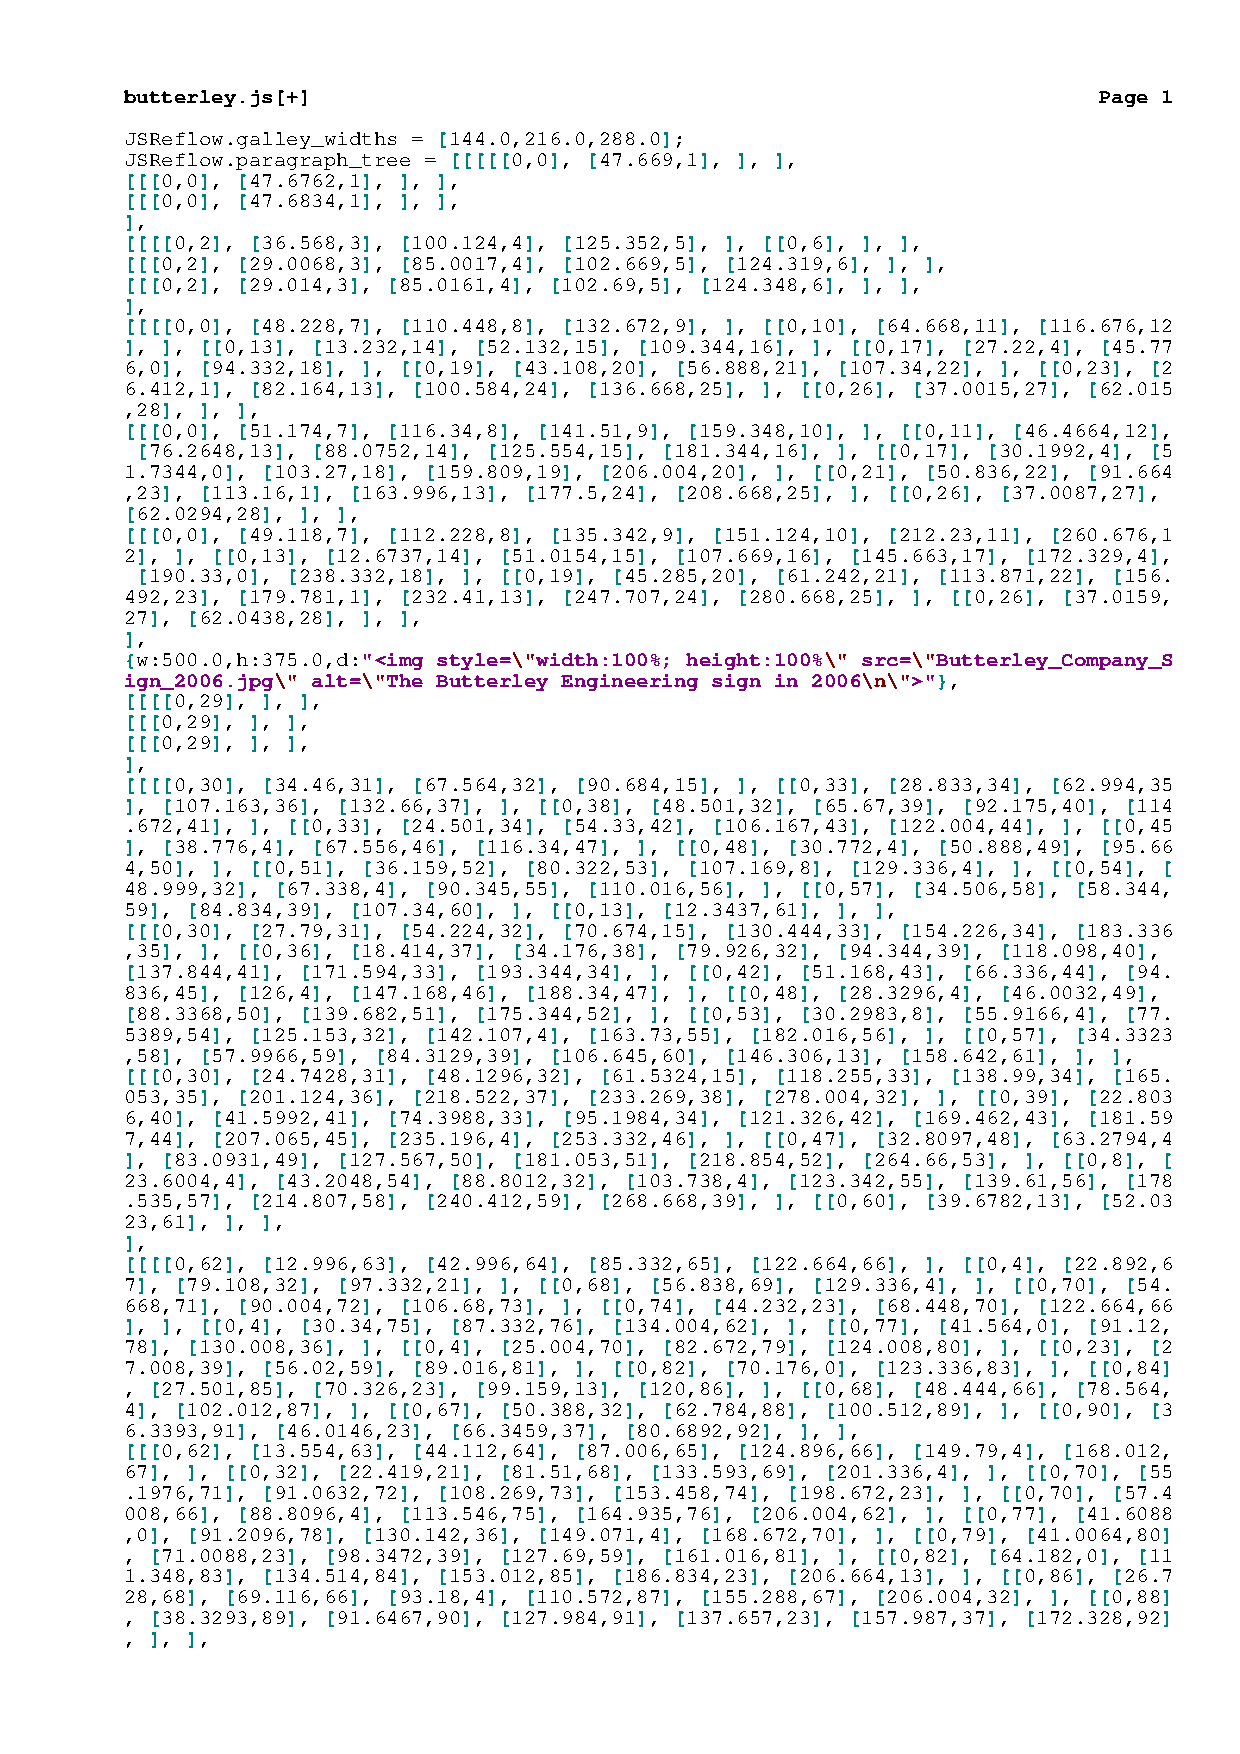
\includepdf[pages=-,scale=.8,pagecommand={}]{butterley.pdf}



\cleardoublepage
\chapter{Sample Layouts}
\label{app:layouts}

All the layouts in this section are of the author's 2011 paper, \emph{Reflowable Documents Composed from Prerendered Atomic Components} \cite{Pinkney2011}.

All the Malleable Document System layouts use the same selection of galley renderings as were used in Rendering D of the user study\ed see Table~\ref{tab:galleypool} on page~\pageref{tab:galleypool}.


\newpage

\section{Layout by the Malleable Document System}

\newlength{\imgwid}

\subsection{Rendered by Mozilla Firefox on a PC}
\label{app:layout-ff}

\cite{Pinkney2011} laid out by the malleable document system, running in Mozilla Firefox on a PC. The page size has been selected to resemble that of A4 paper in a portrait orientation.

\begin{center}
\setlength{\imgwid}{0.47\textwidth}
\fbox{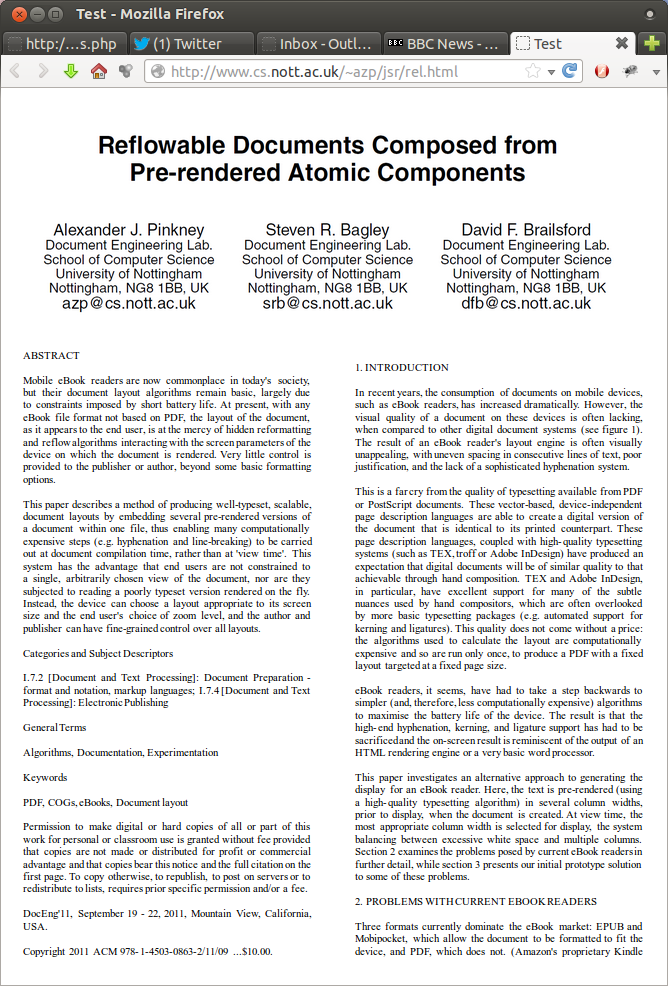
\includegraphics[trim=0in 0in 0in 1.2in, clip=true, width=\imgwid]{gfx/p1}}\hspace{0.01\textwidth}
\fbox{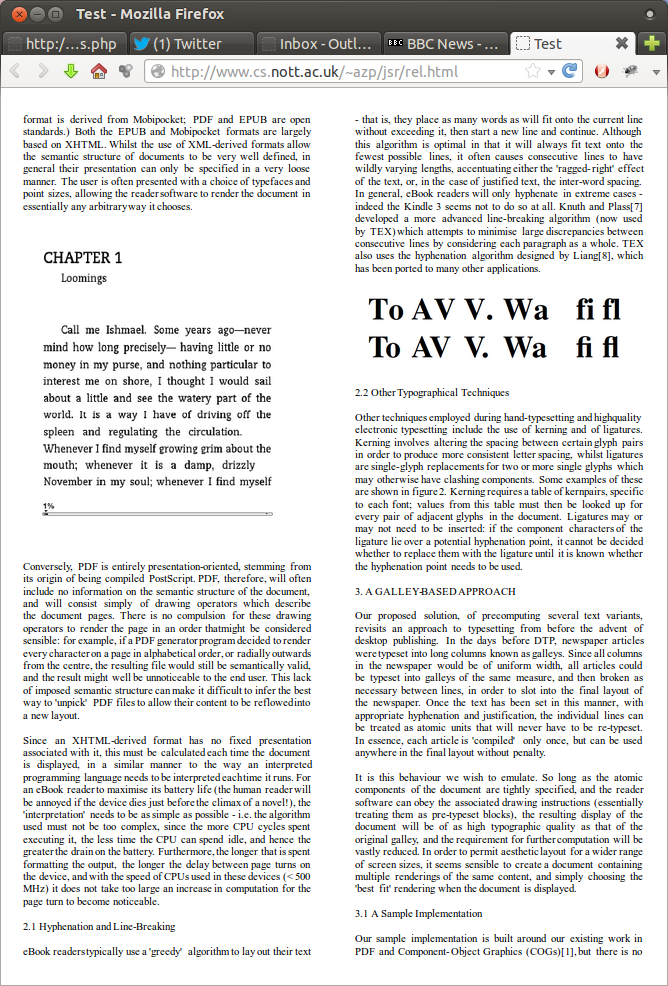
\includegraphics[trim=0in 0in 0in 1.2in, clip=true, width=\imgwid]{gfx/p2}}

\vspace{0.2in}
\fbox{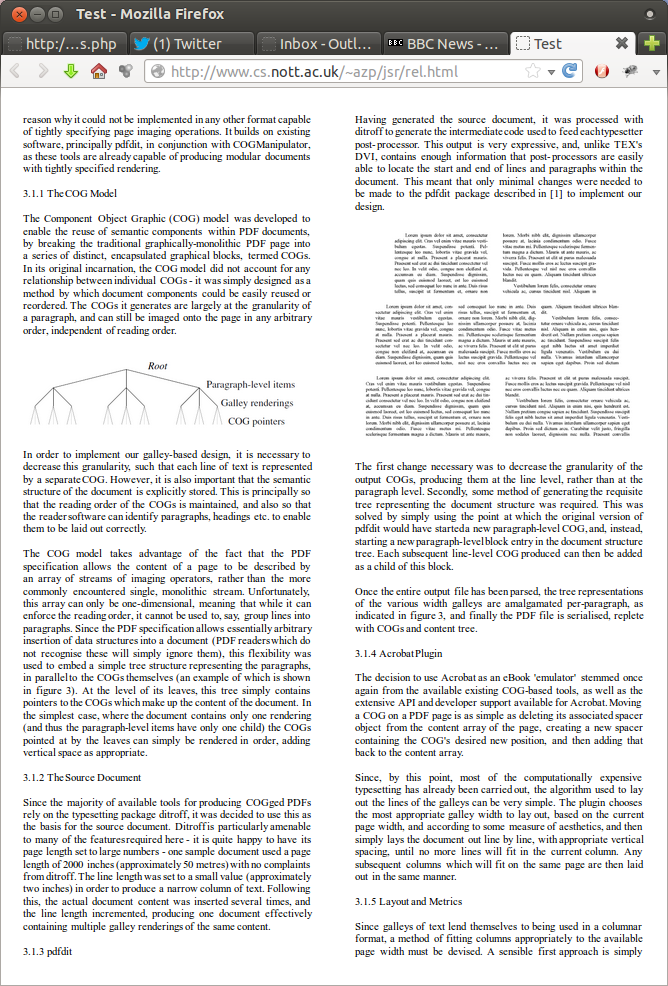
\includegraphics[trim=0in 0in 0in 1.2in, clip=true, width=\imgwid]{gfx/p3}}\hspace{0.01\textwidth}
\fbox{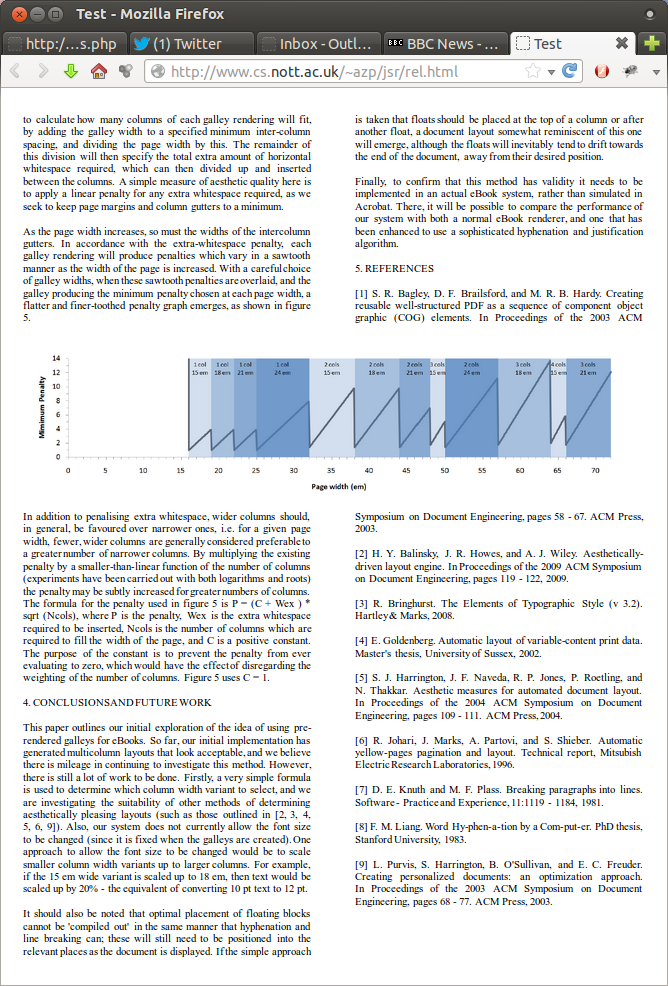
\includegraphics[trim=0in 0in 0in 1.2in, clip=true, width=\imgwid]{gfx/p4}}
\end{center}


\clearpage


\cite{Pinkney2011} laid out by the malleable document system, running in Mozilla Firefox on a PC. The page size has been selected to resemble that of A4 paper in a landscape orientation.

\begin{center}
\setlength{\imgwid}{0.45\textwidth}
\fbox{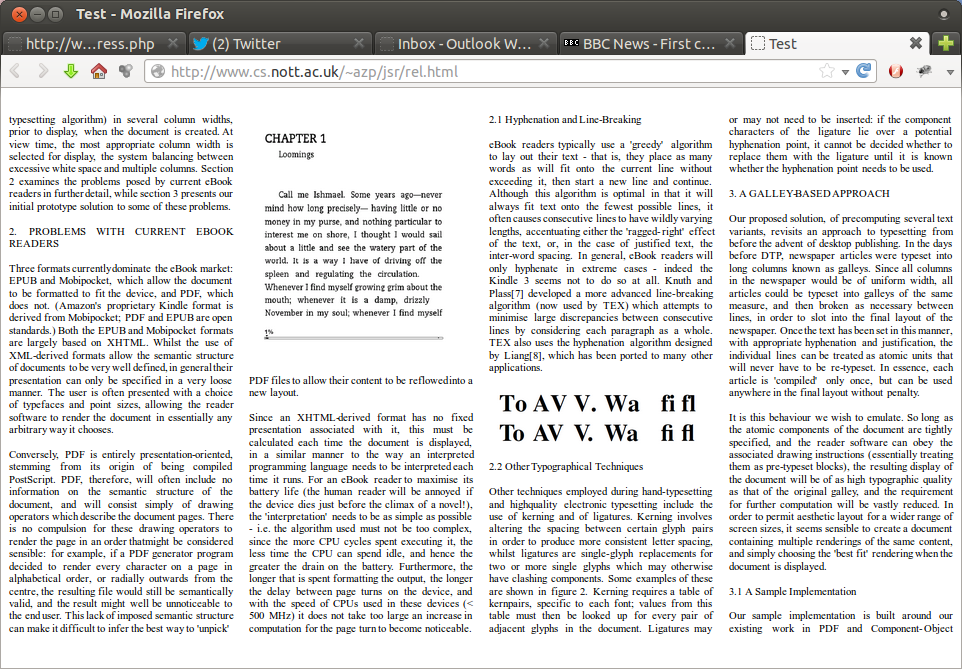
\includegraphics[trim=0in 0in 0in 1.2in, clip=true, angle=90, width=\imgwid]{gfx/q2}}\hspace{0.05\textwidth}
\fbox{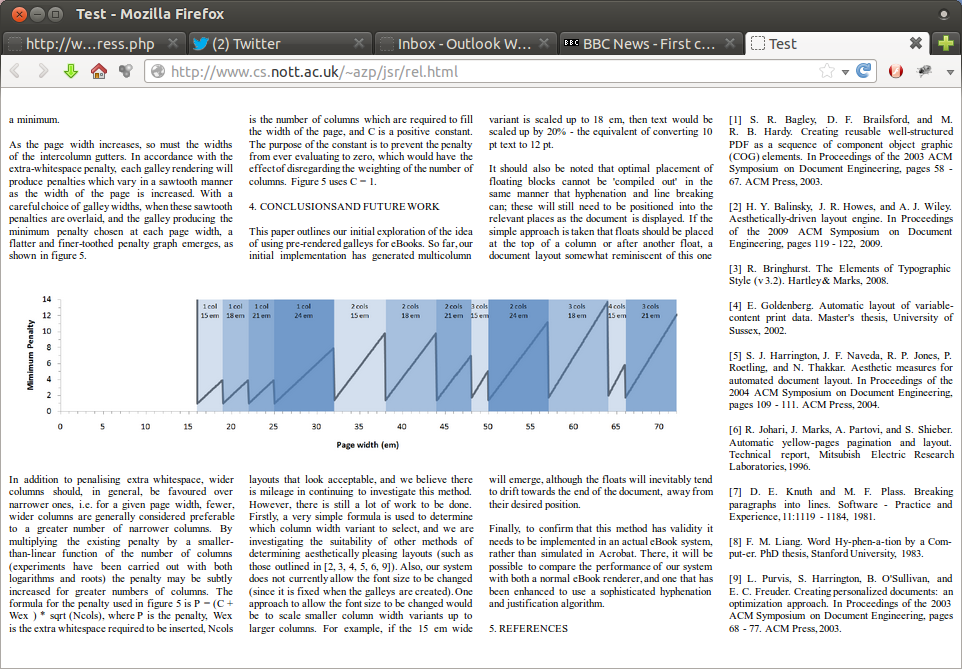
\includegraphics[trim=0in 0in 0in 1.2in, clip=true, angle=90, width=\imgwid]{gfx/q4}}

\vspace{0.2in}
\fbox{
\includegraphics[trim=0in 0in 0in 1.2in, clip=true, angle=90, width=\imgwid]{gfx/q1}}\hspace{0.05\textwidth}
\fbox{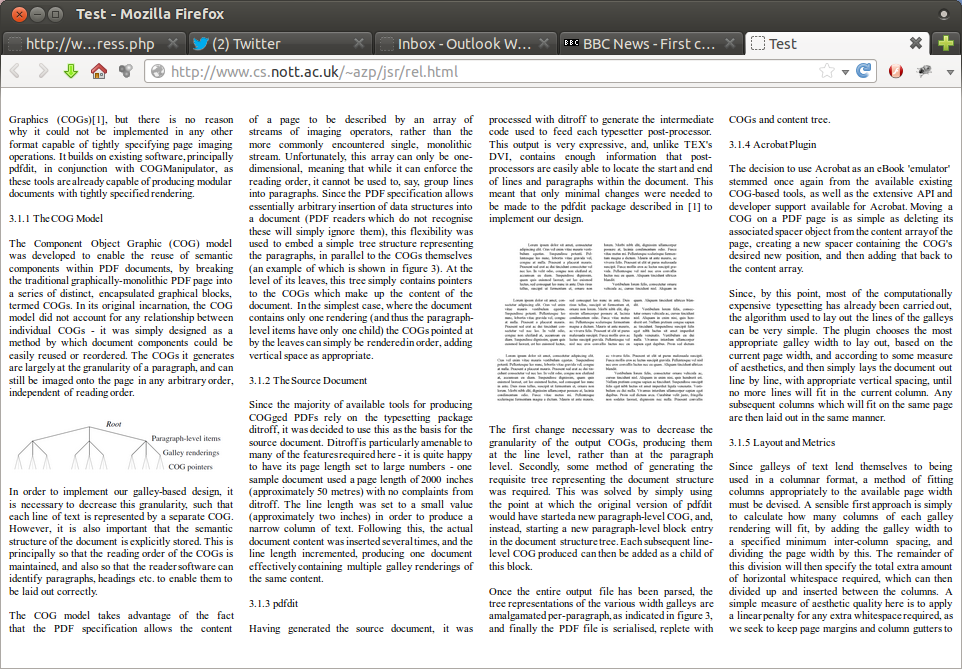
\includegraphics[trim=0in 0in 0in 1.2in, clip=true, angle=90, width=\imgwid]{gfx/q3}}
\end{center}


\clearpage


\cite{Pinkney2011} laid out by the malleable document system, running in Mozilla Firefox on a PC. The page size has been selected to resemble that of an \ebook{} reader in a portrait orientation.

\label{app:p:layout-ff-ereader}
\begin{center}
\setlength{\imgwid}{0.26\textwidth}
\fbox{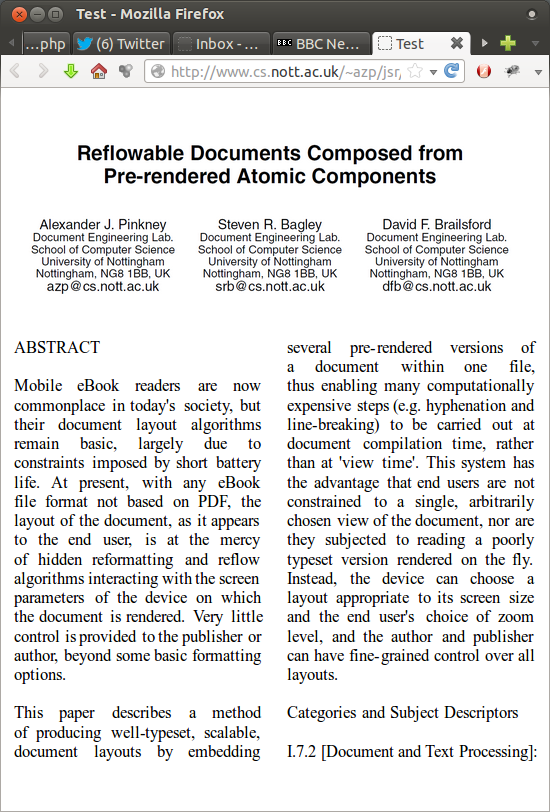
\includegraphics[trim=0in 0in 0in 1.2in, clip=true, width=\imgwid]{gfx/r1}}
\fbox{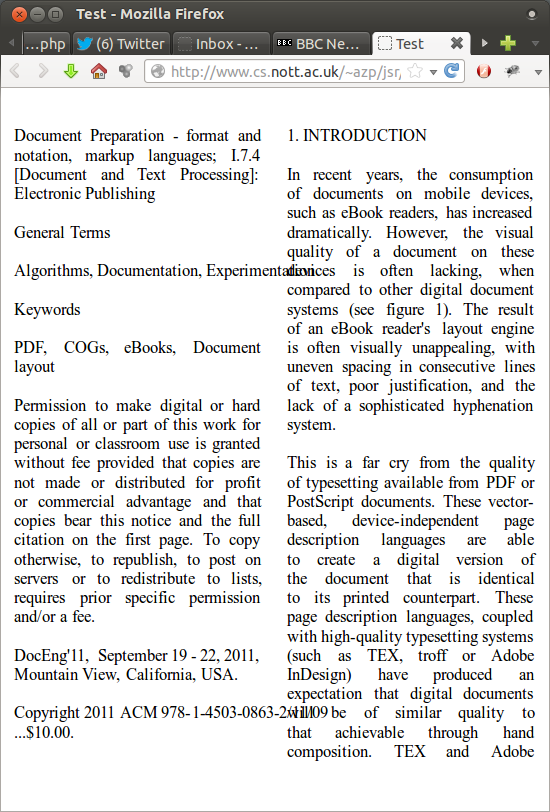
\includegraphics[trim=0in 0in 0in 1.2in, clip=true, width=\imgwid]{gfx/r2}}
\fbox{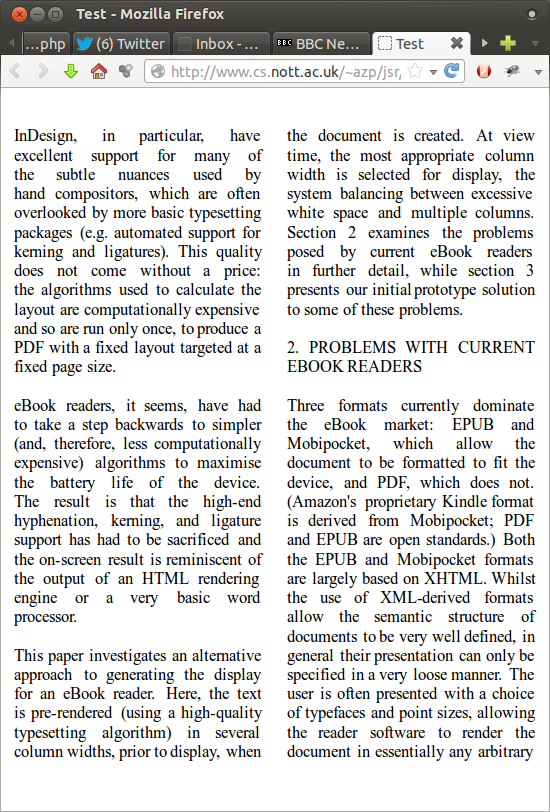
\includegraphics[trim=0in 0in 0in 1.2in, clip=true, width=\imgwid]{gfx/r3}}
\fbox{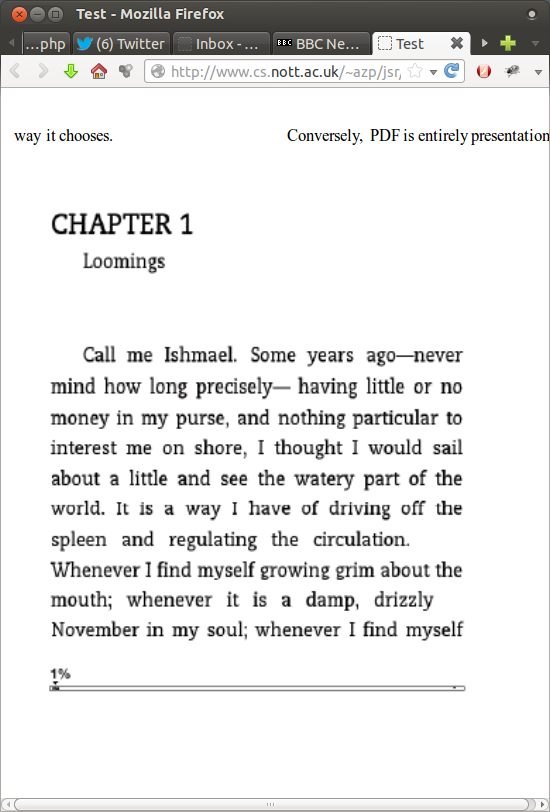
\includegraphics[trim=0in 0in 0in 1.2in, clip=true, width=\imgwid]{gfx/r4}}
\fbox{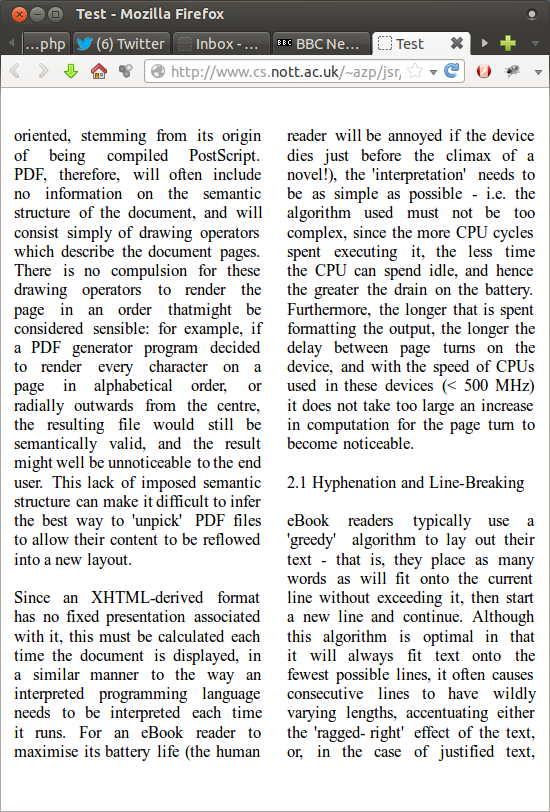
\includegraphics[trim=0in 0in 0in 1.2in, clip=true, width=\imgwid]{gfx/r5}}
\fbox{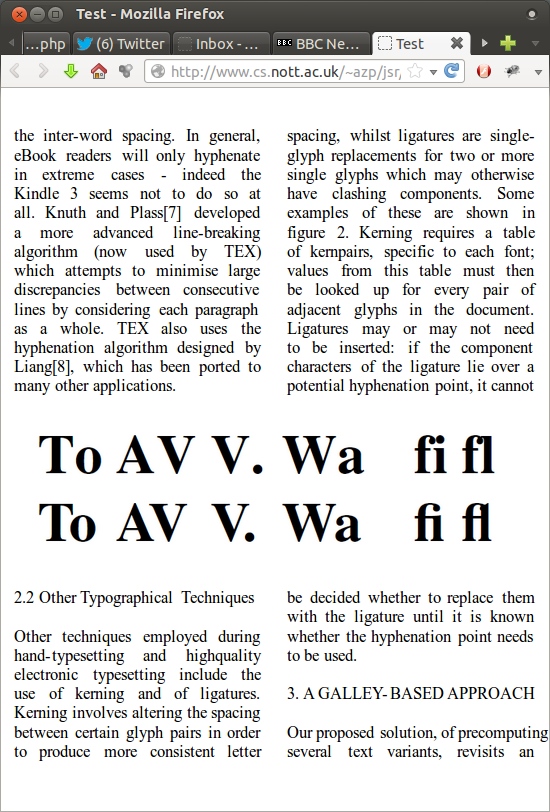
\includegraphics[trim=0in 0in 0in 1.2in, clip=true, width=\imgwid]{gfx/r6}}
\fbox{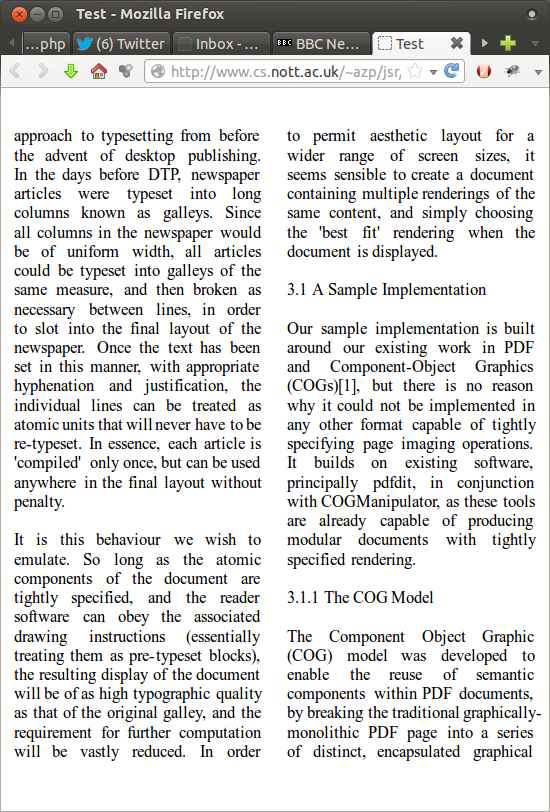
\includegraphics[trim=0in 0in 0in 1.2in, clip=true, width=\imgwid]{gfx/r7}}
\fbox{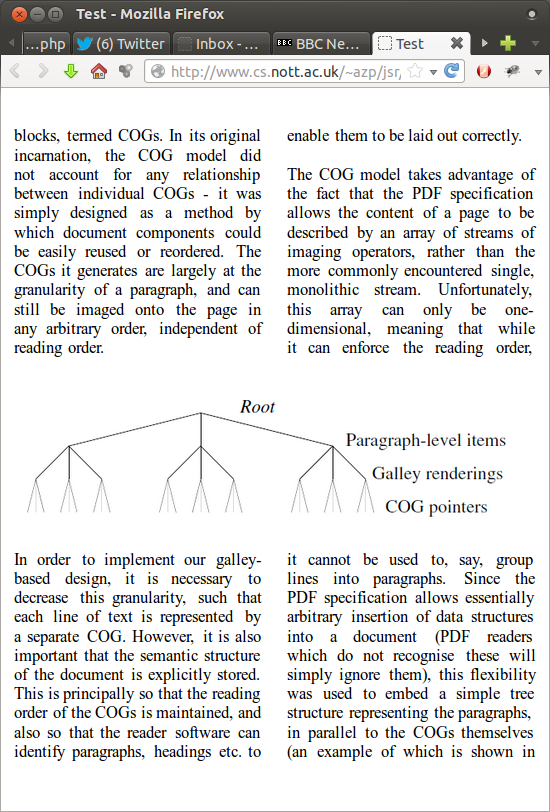
\includegraphics[trim=0in 0in 0in 1.2in, clip=true, width=\imgwid]{gfx/r8}}
\fbox{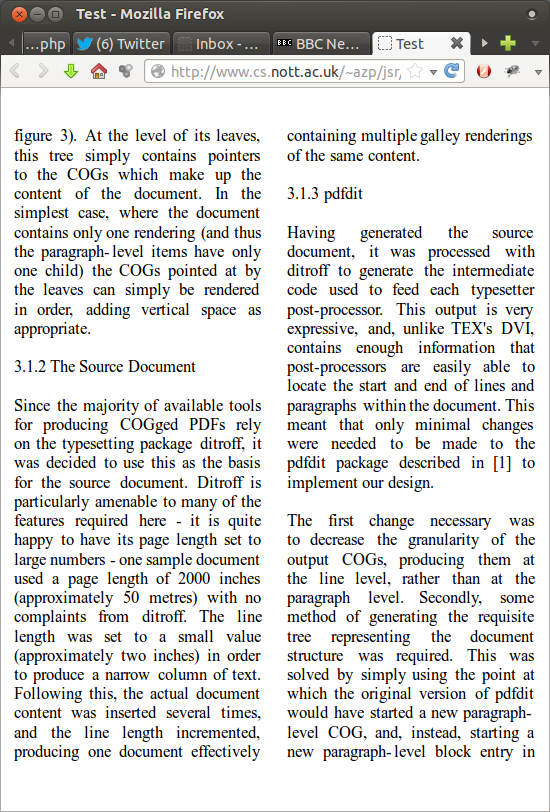
\includegraphics[trim=0in 0in 0in 1.2in, clip=true, width=\imgwid]{gfx/r9}}
\fbox{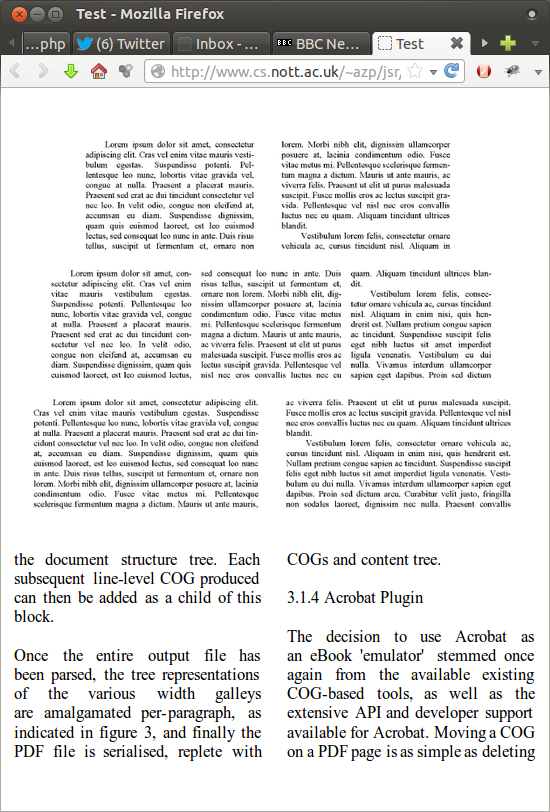
\includegraphics[trim=0in 0in 0in 1.2in, clip=true, width=\imgwid]{gfx/r10}}
\fbox{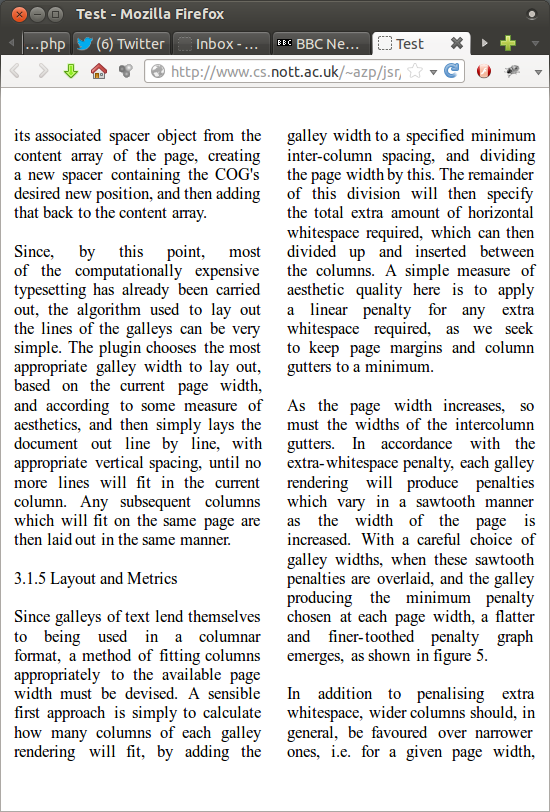
\includegraphics[trim=0in 0in 0in 1.2in, clip=true, width=\imgwid]{gfx/r11}}
\fbox{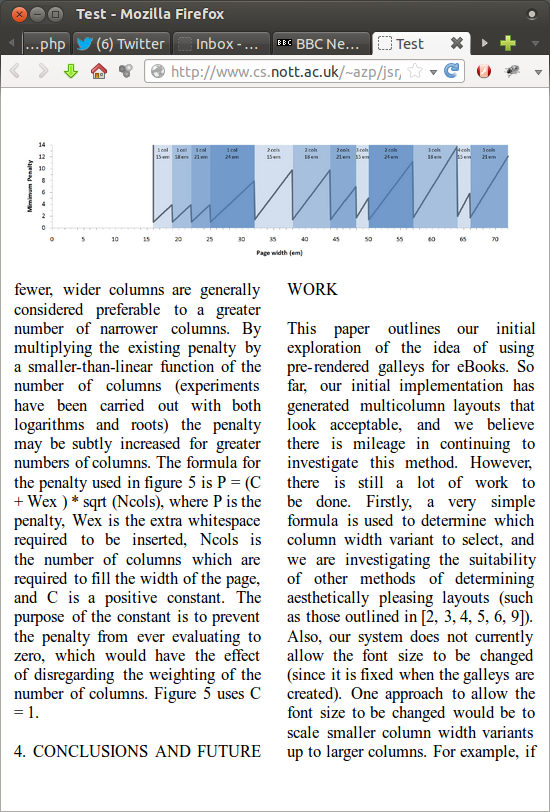
\includegraphics[trim=0in 0in 0in 1.2in, clip=true, width=\imgwid]{gfx/r12}}
\fbox{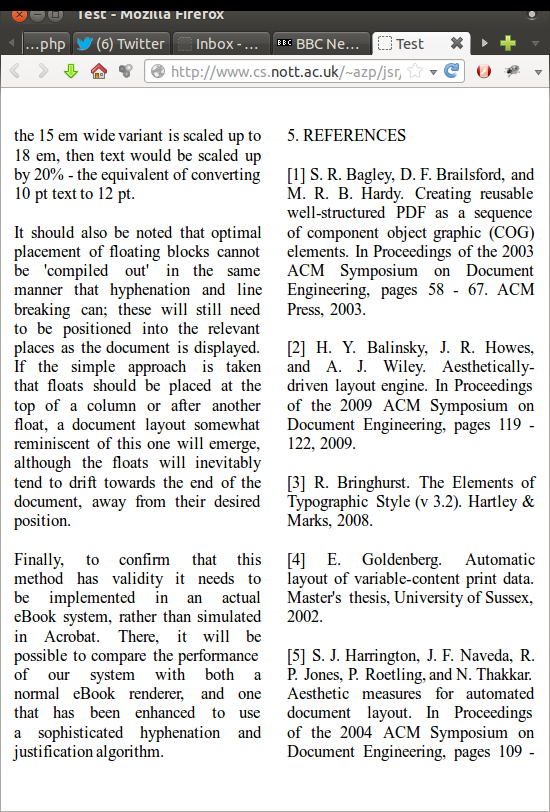
\includegraphics[trim=0in 0in 0in 1.2in, clip=true, width=\imgwid]{gfx/r13}}
\fbox{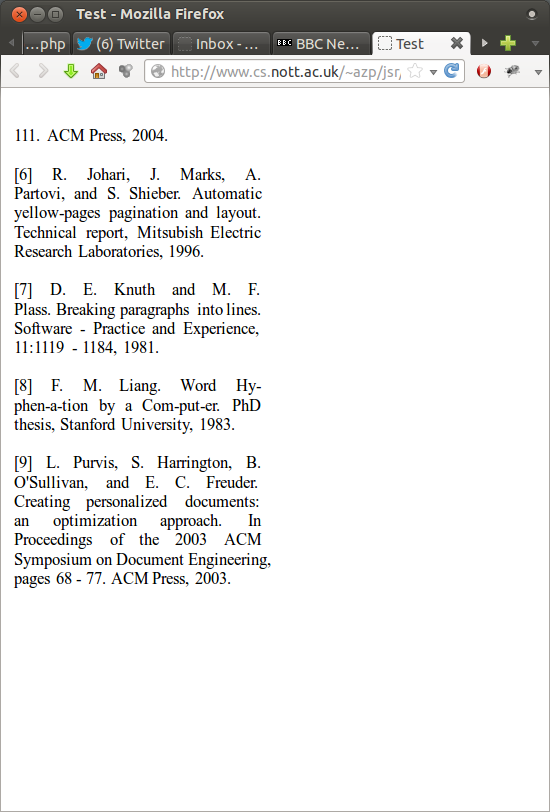
\includegraphics[trim=0in 0in 0in 1.2in, clip=true, width=\imgwid]{gfx/r14}}
\end{center}


\clearpage


\subsection{Chrome on an Android Phone}
\label{app:layout-android}


\cite{Pinkney2011} laid out by the malleable document system, running in Chrome on an Android phone. This example shows a point size that is a little on the small side, but is still readable.

\begin{center}
\setlength{\imgwid}{0.3\textwidth}
\fbox{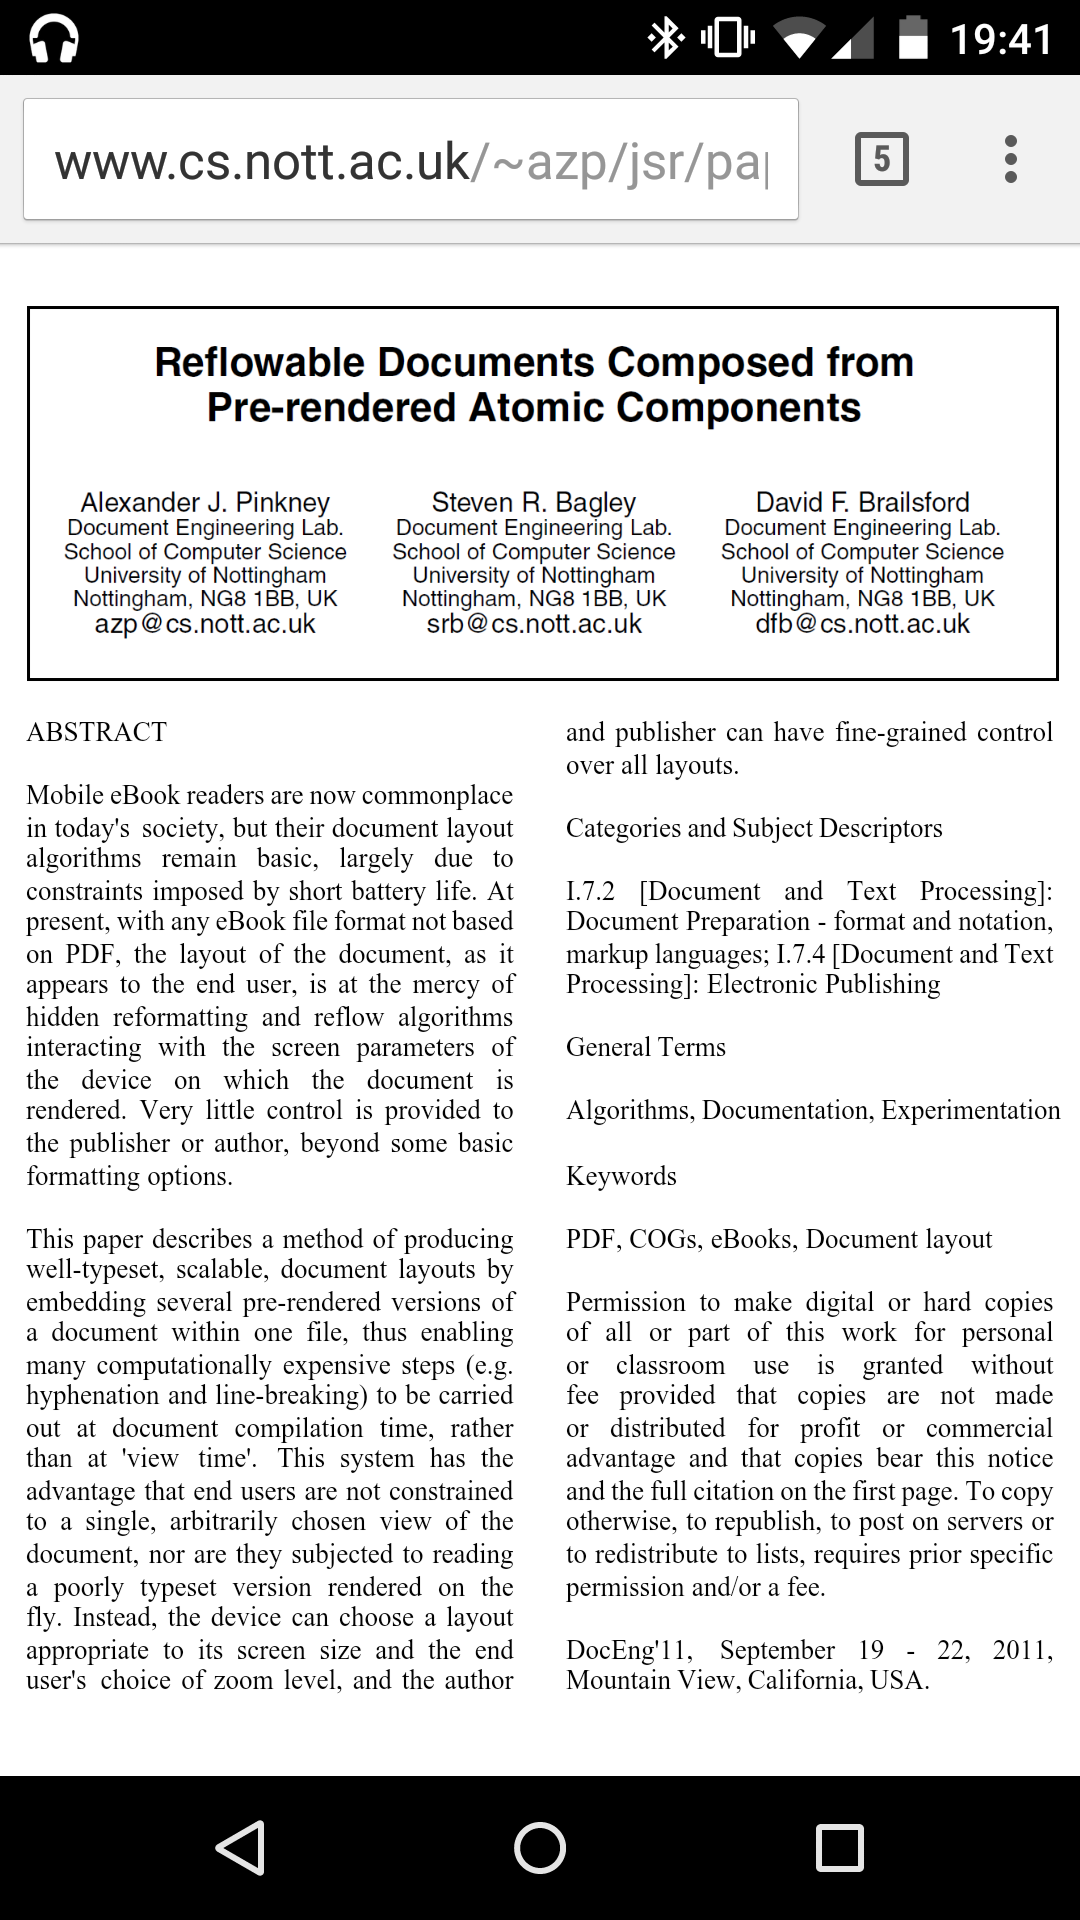
\includegraphics[width=\imgwid]{gfx/n5_1_01}}
\fbox{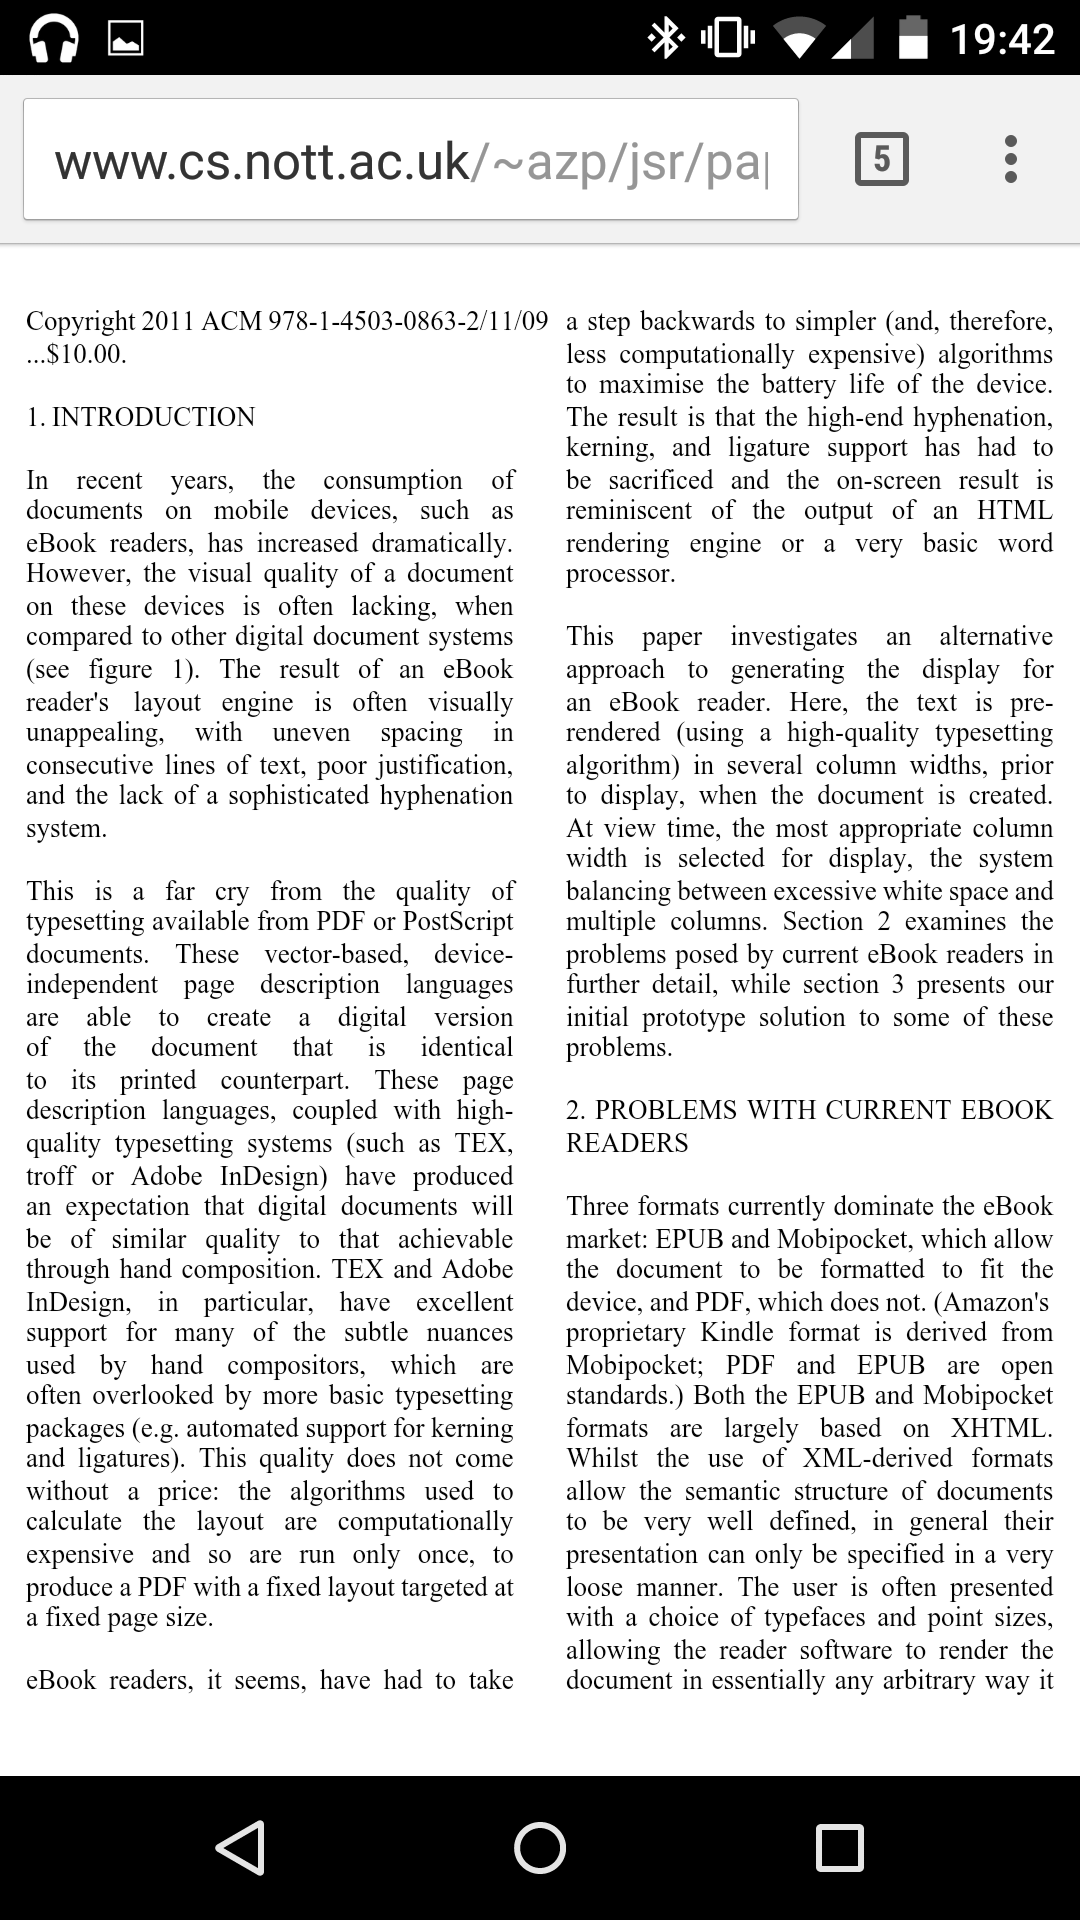
\includegraphics[width=\imgwid]{gfx/n5_1_02}}
\fbox{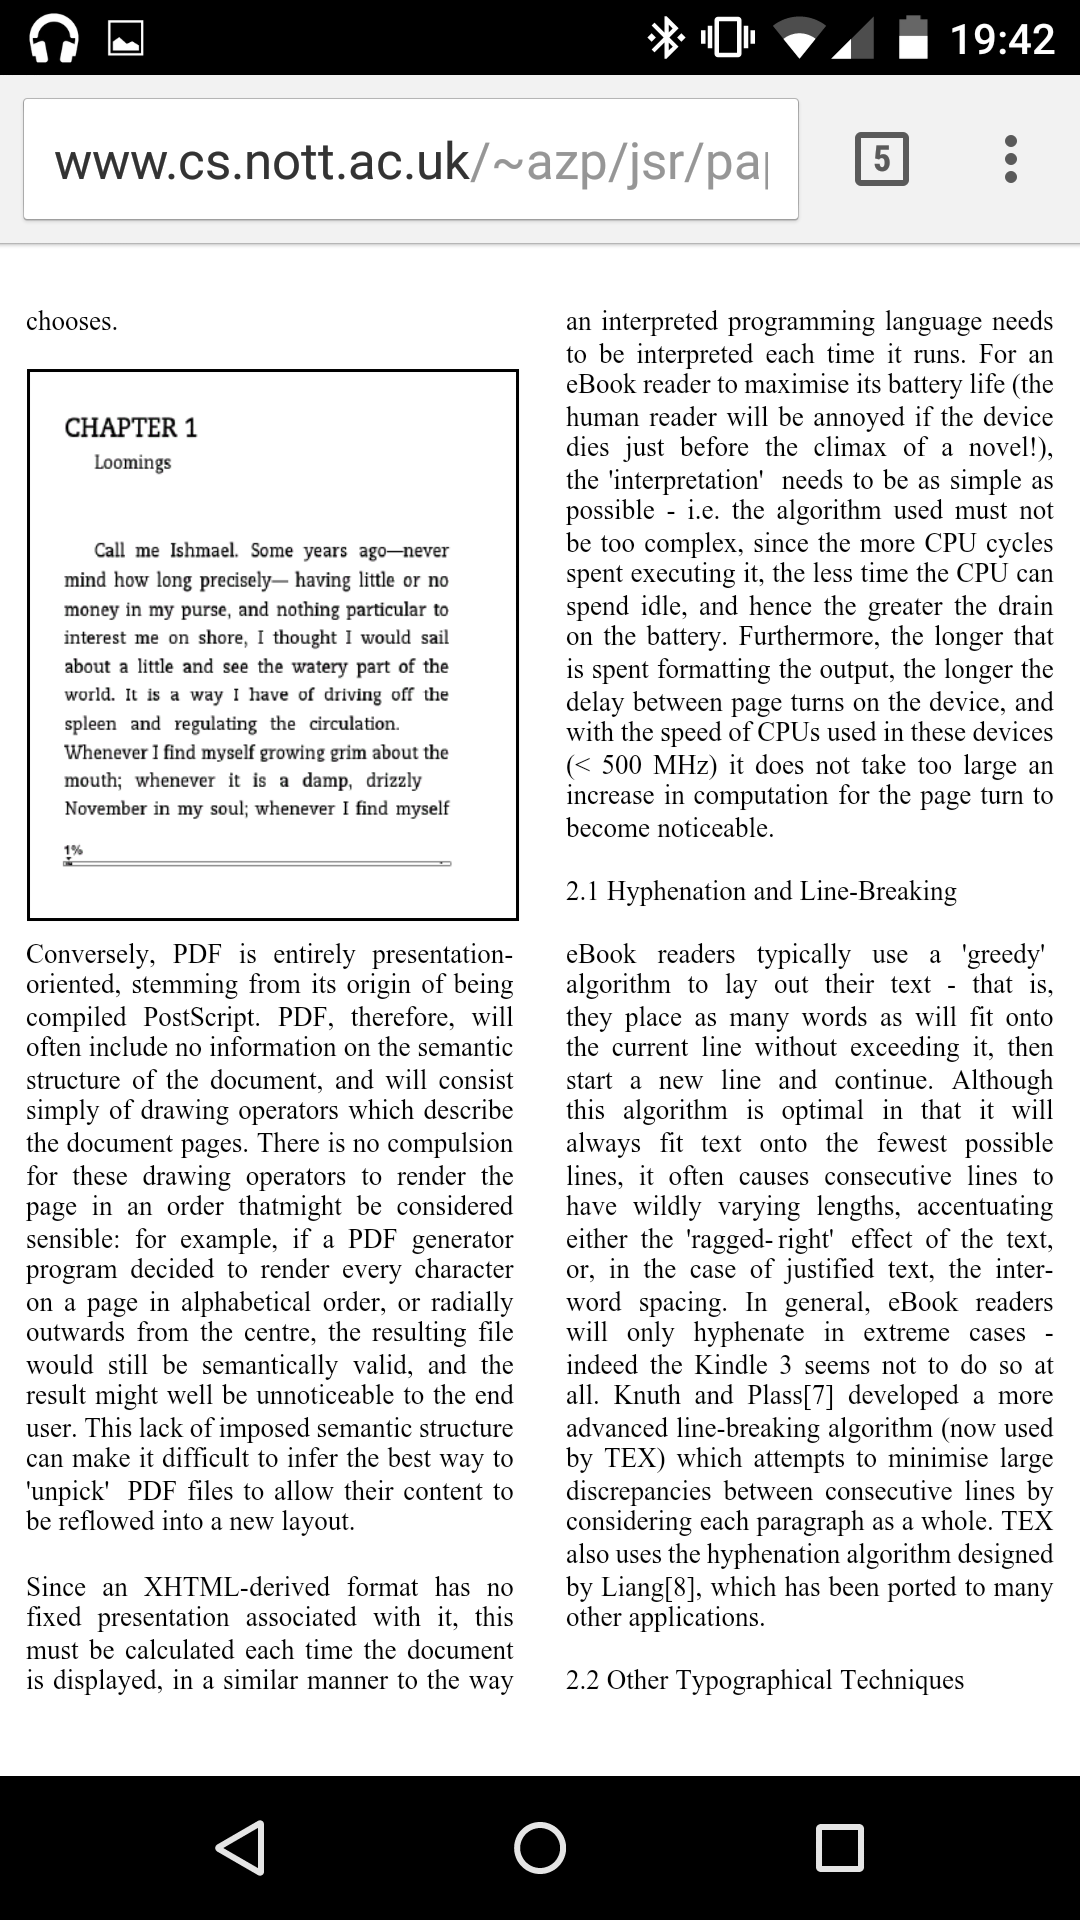
\includegraphics[width=\imgwid]{gfx/n5_1_03}}
\fbox{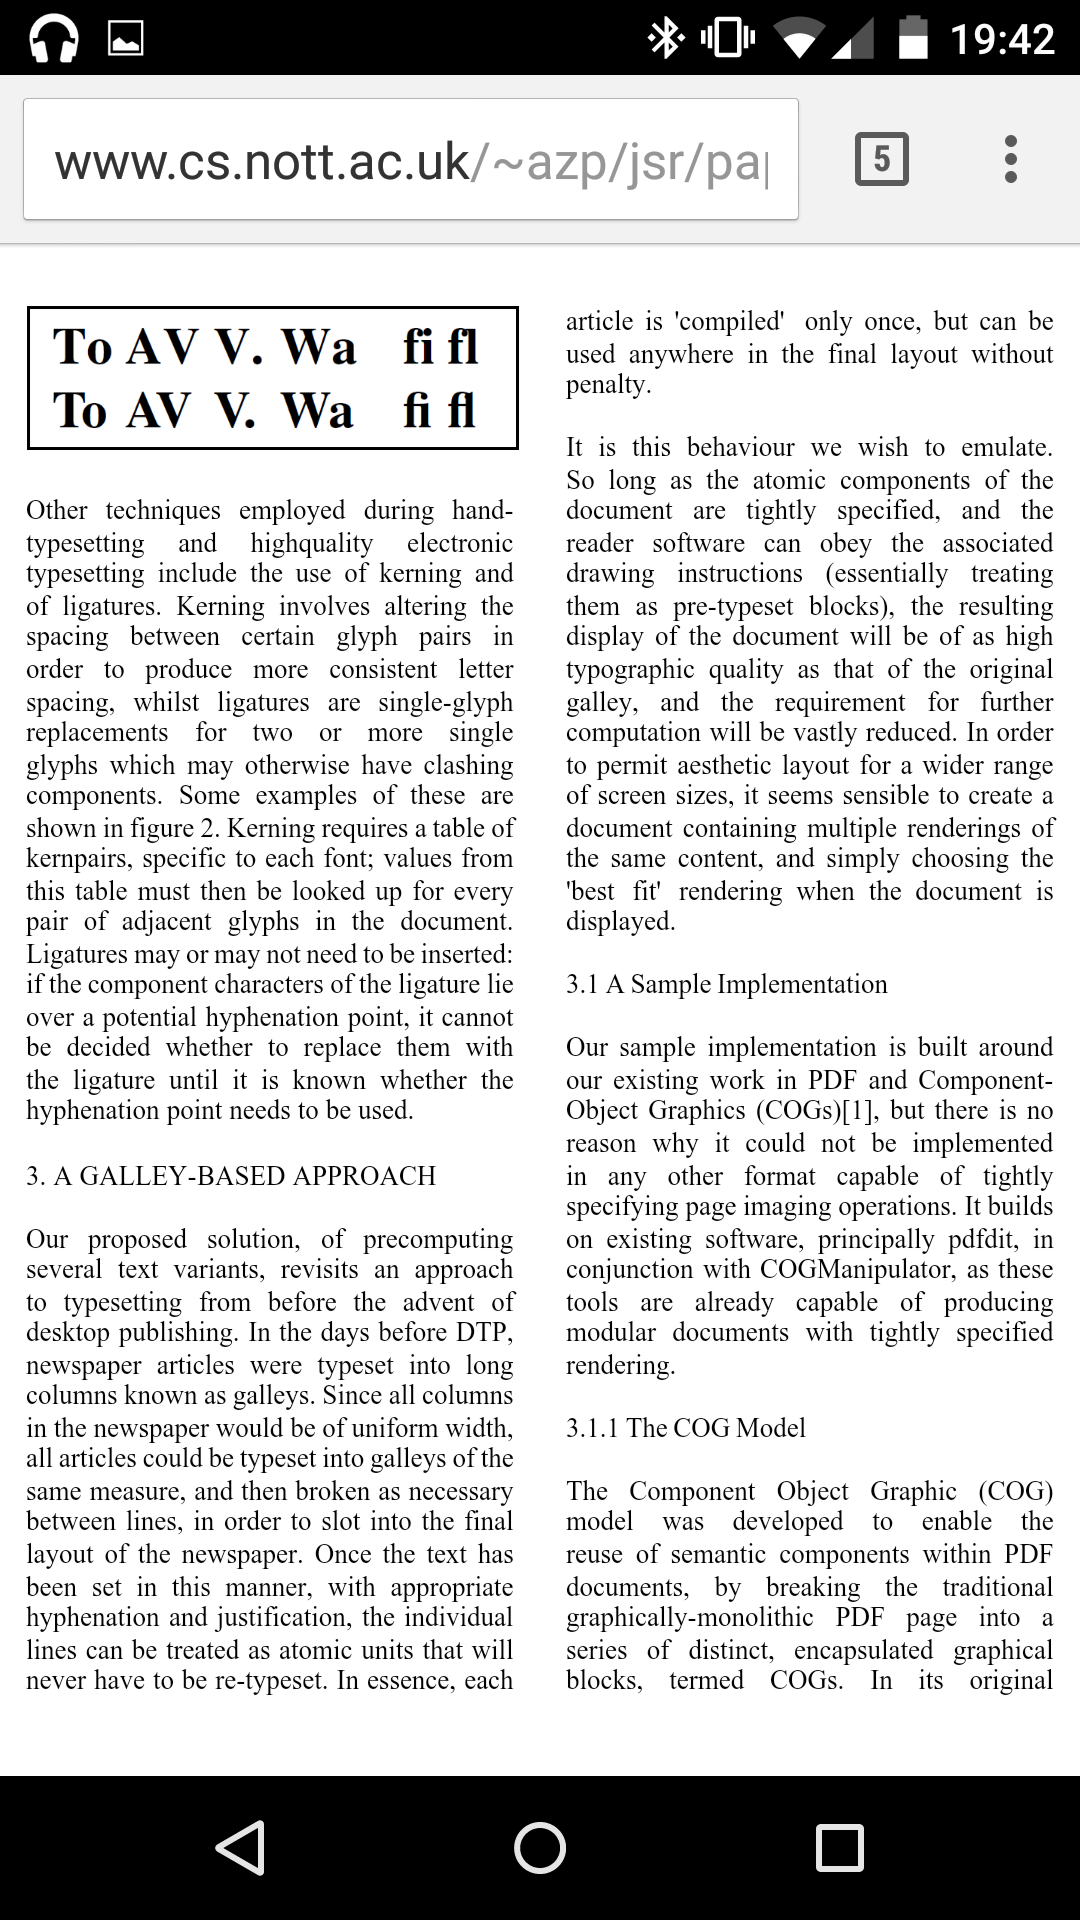
\includegraphics[width=\imgwid]{gfx/n5_1_04}}
\fbox{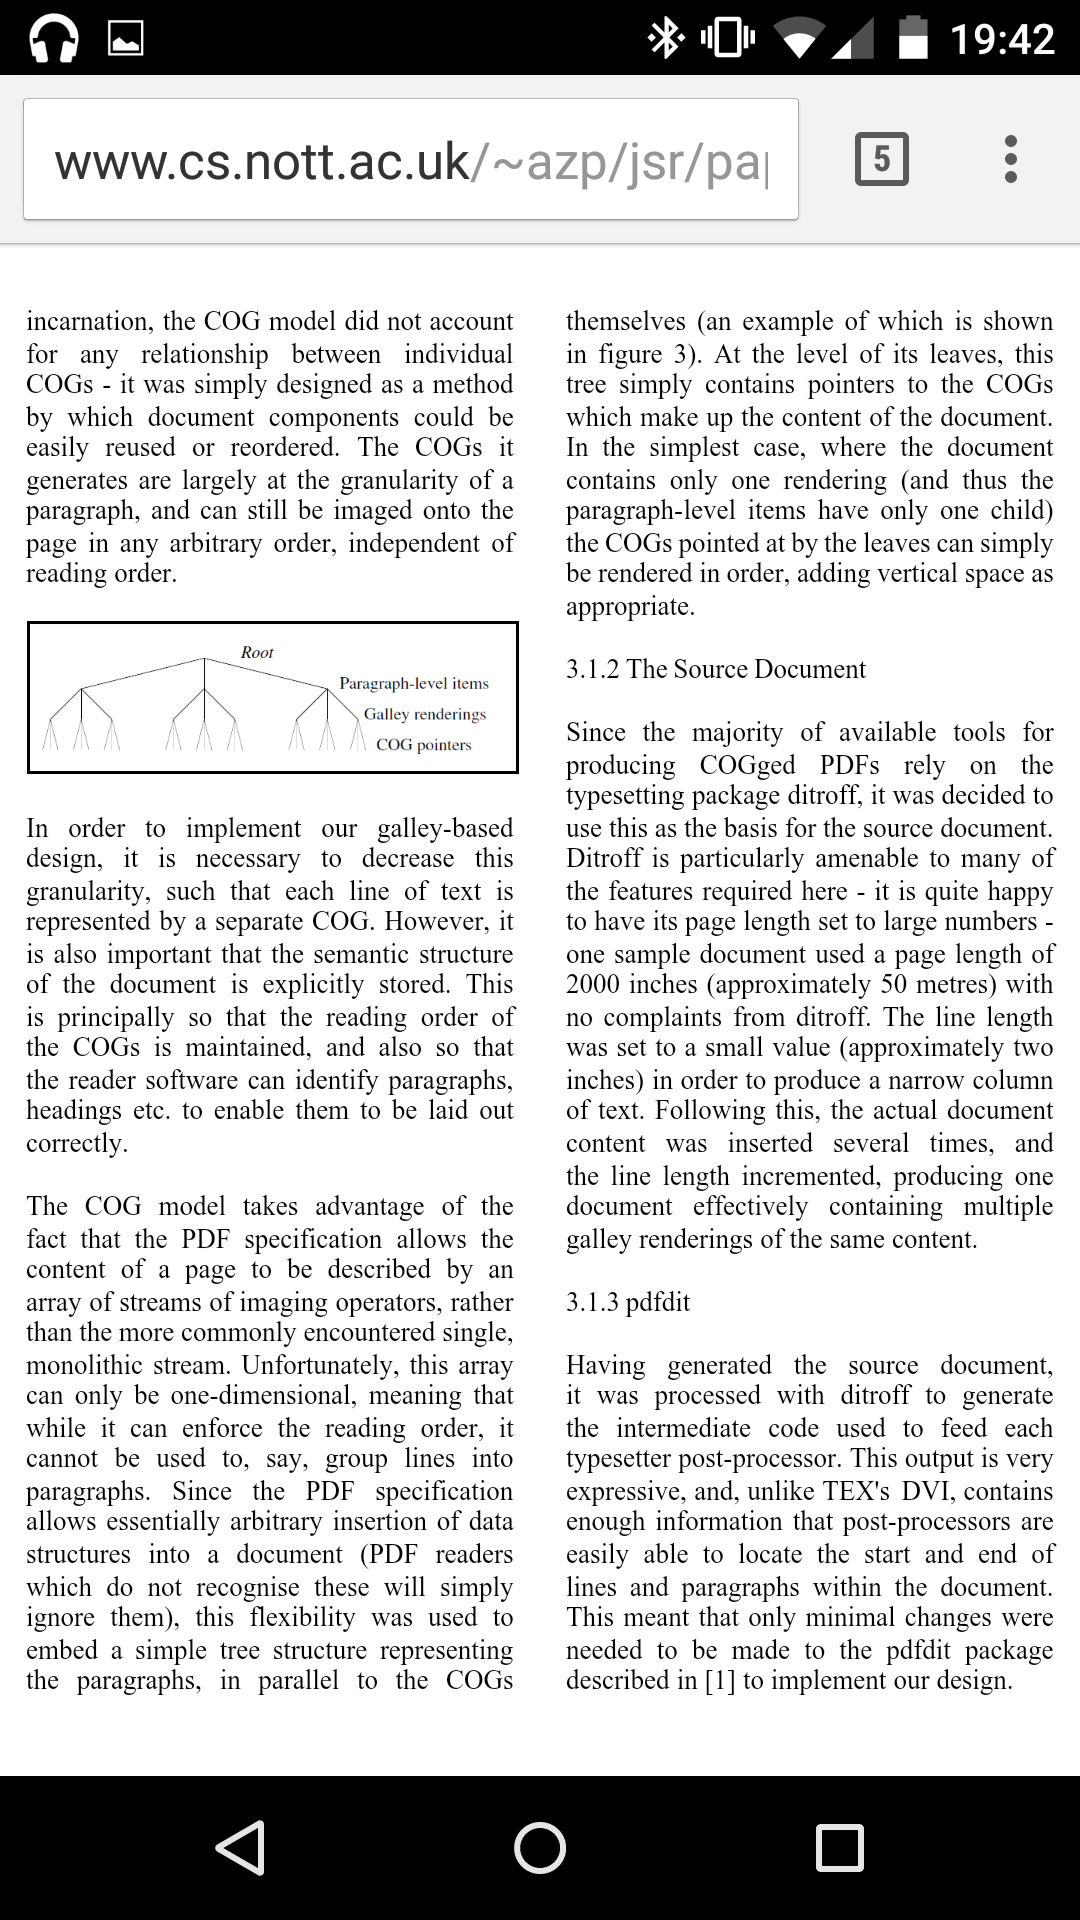
\includegraphics[width=\imgwid]{gfx/n5_1_05}}
\fbox{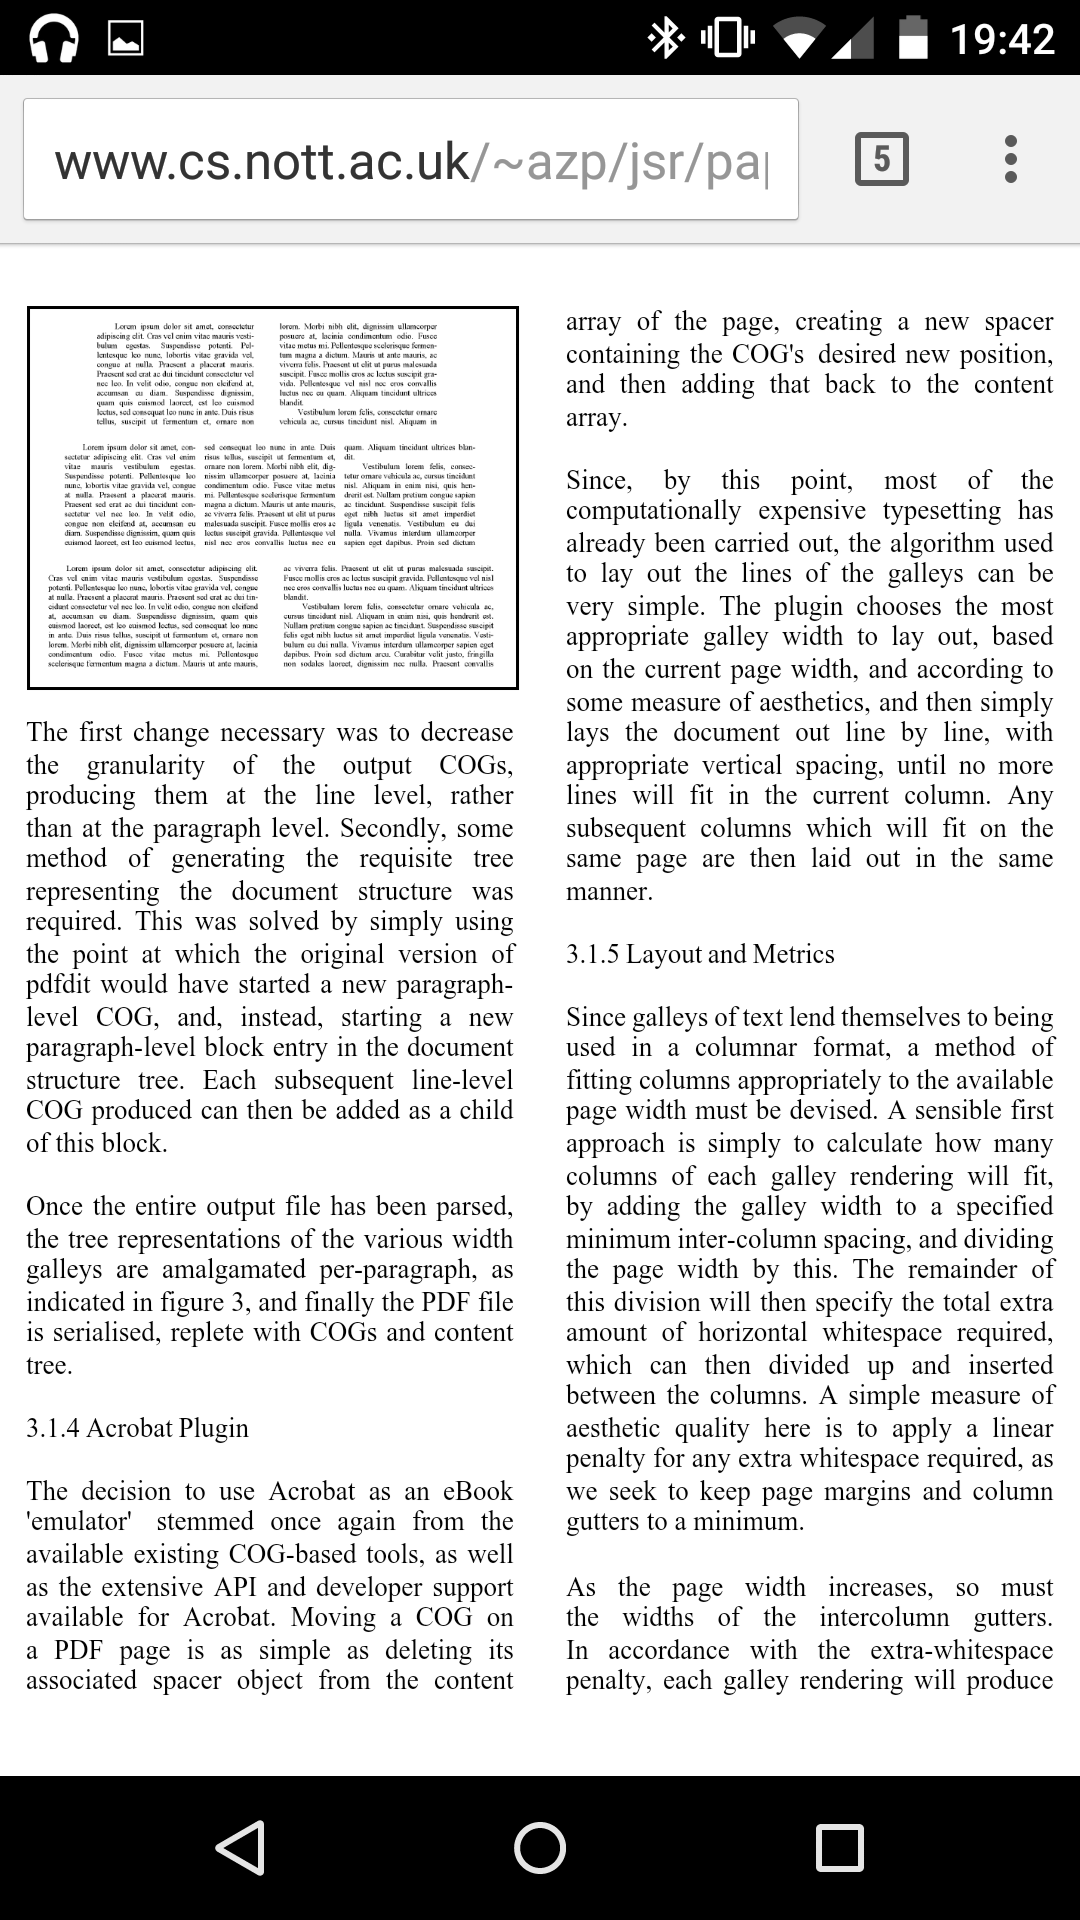
\includegraphics[width=\imgwid]{gfx/n5_1_06}}
\fbox{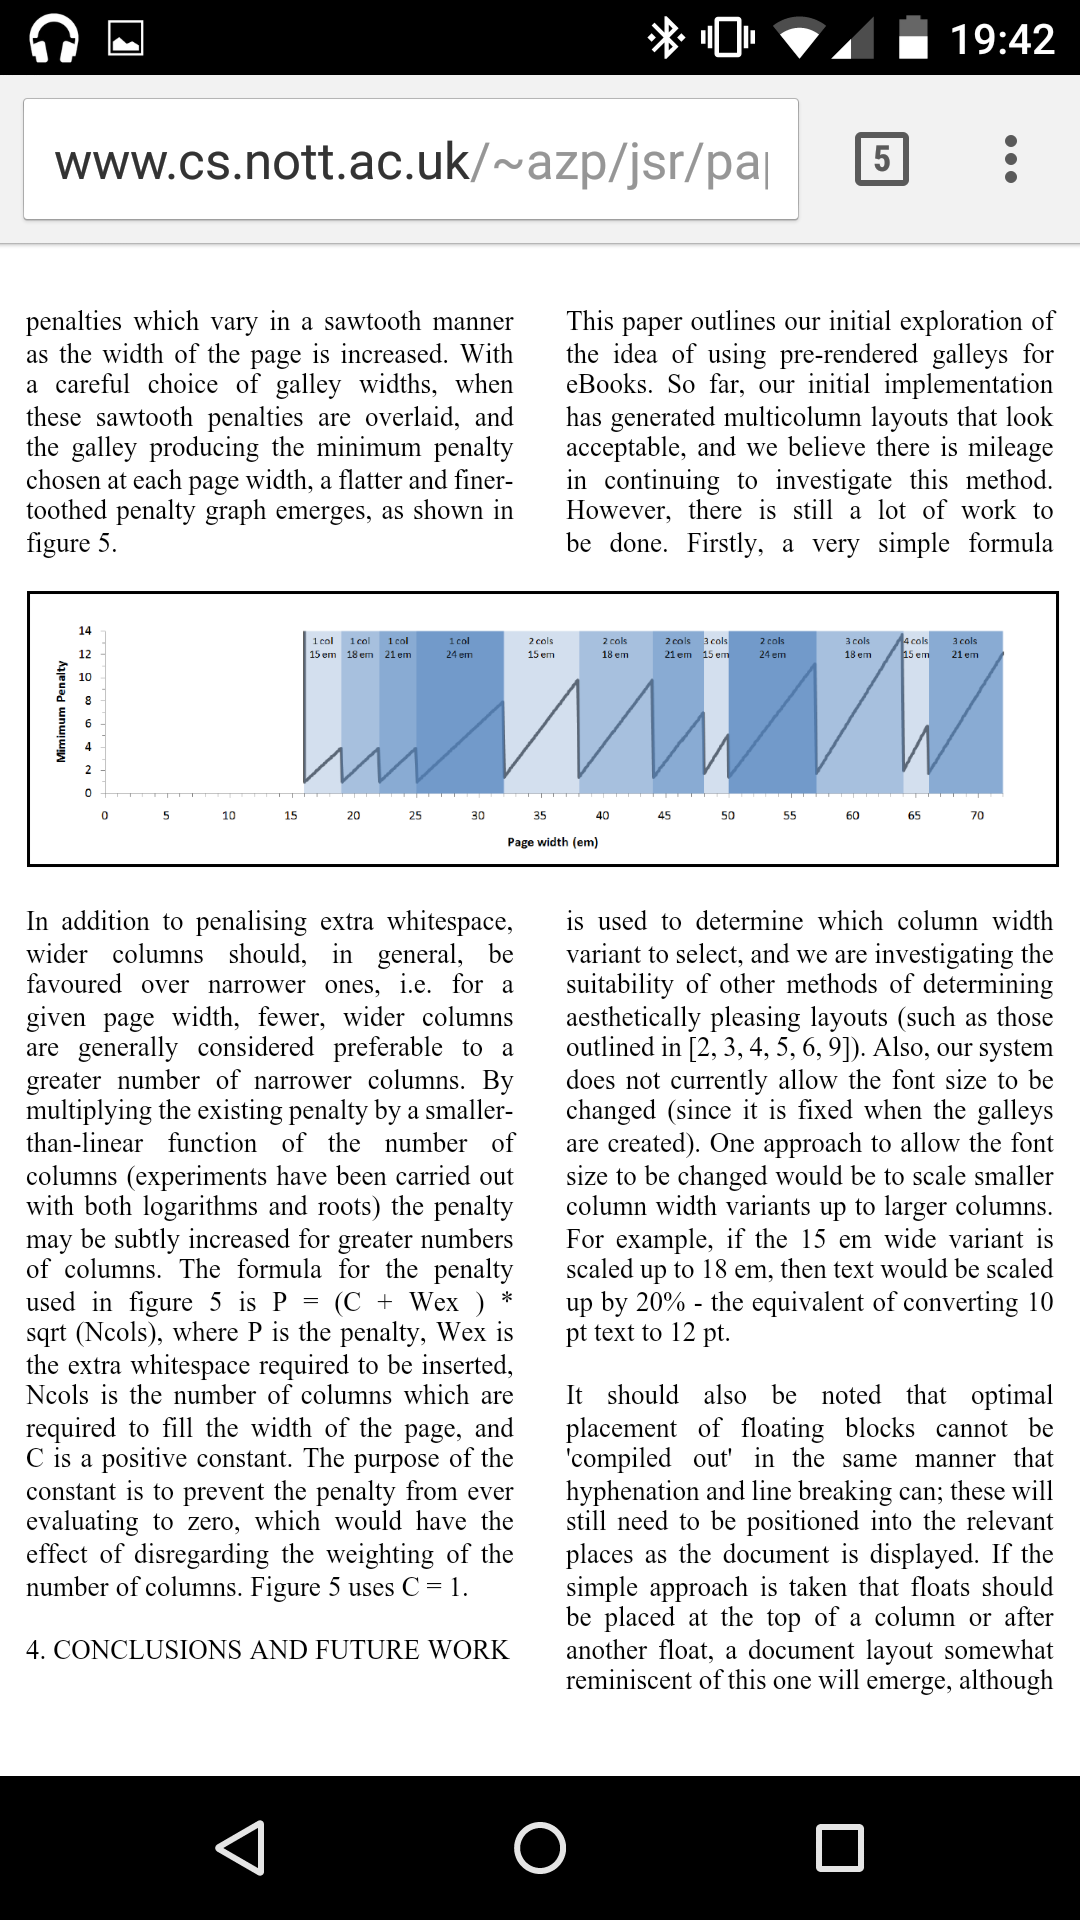
\includegraphics[width=\imgwid]{gfx/n5_1_07}}
\fbox{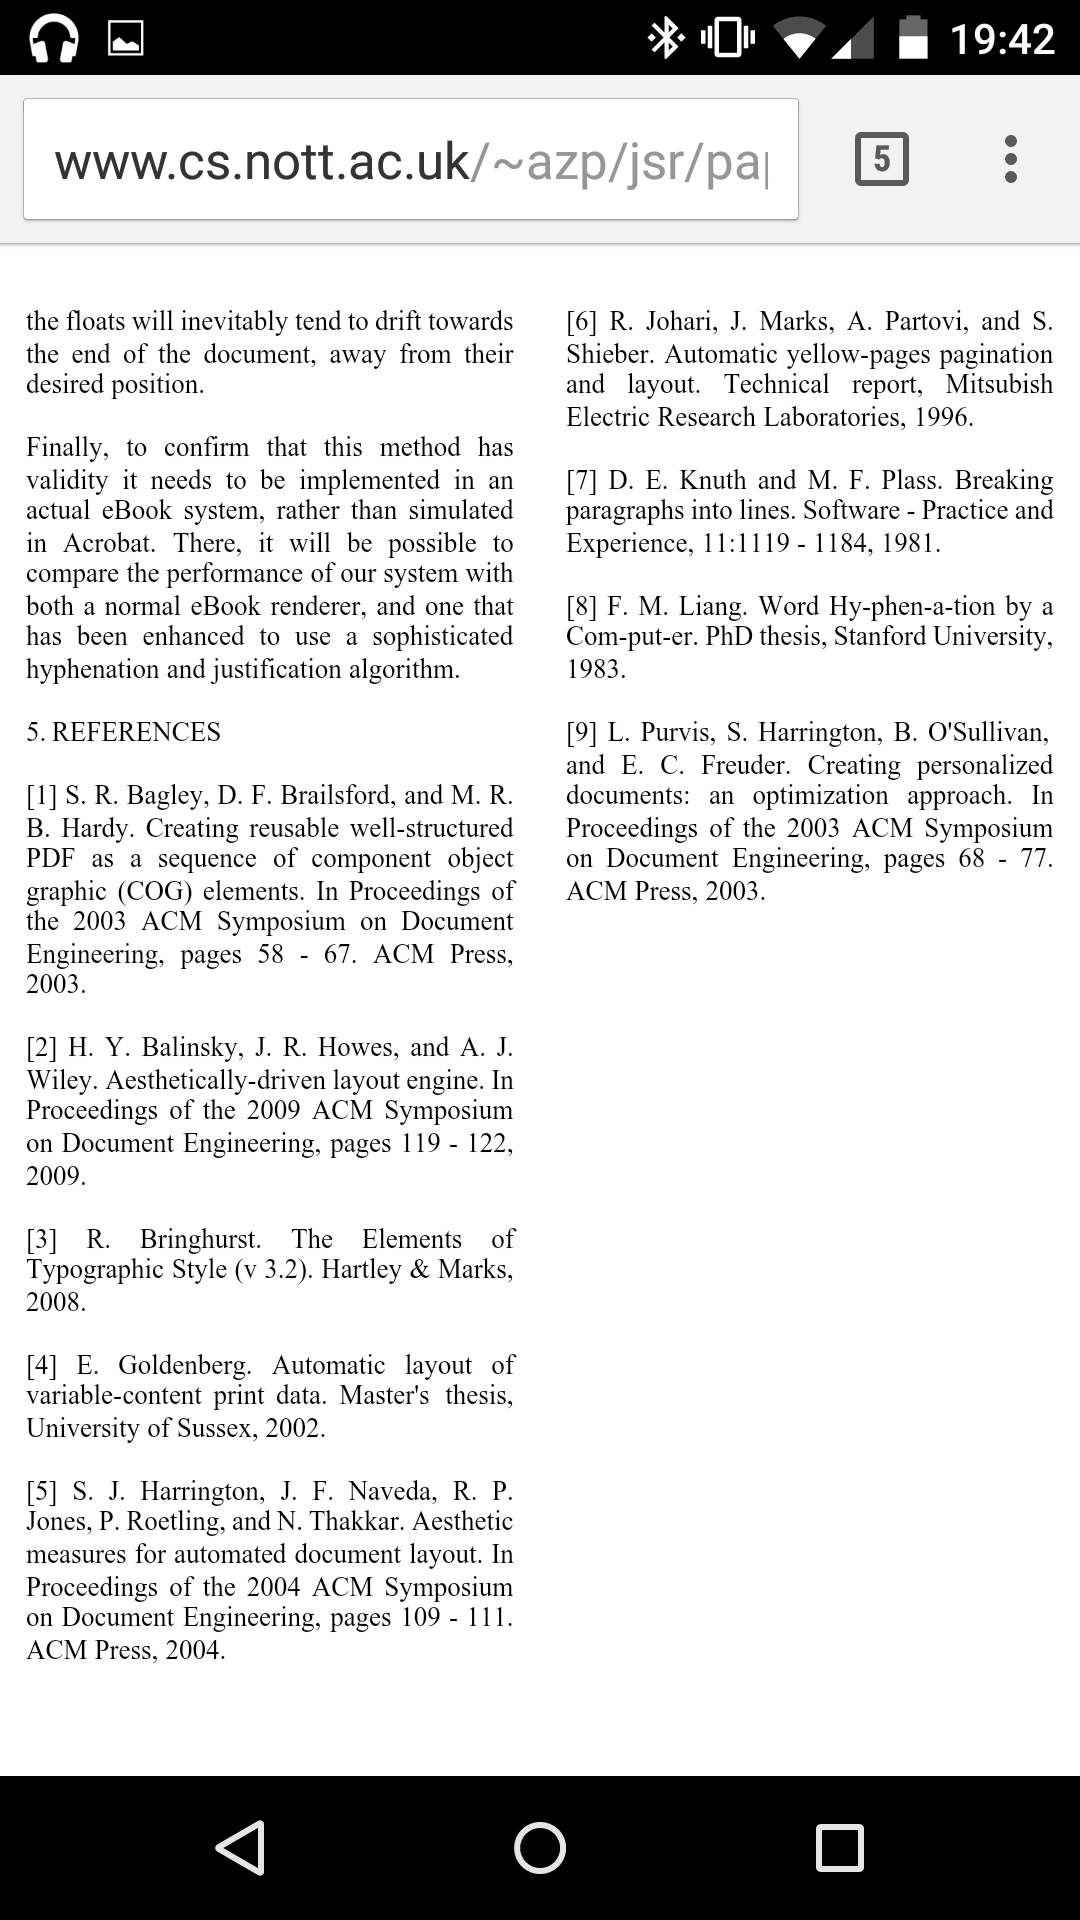
\includegraphics[width=\imgwid]{gfx/n5_1_08}}
\end{center}
 

\clearpage

\cite{Pinkney2011} laid out by the malleable document system, running in Chrome on an Android phone, in portrait and in landscape. This example uses a point size that is likely to be readable by a greater range of people. For brevity's sake, only the first three pages of each rendering are shown.

\begin{center}
\setlength{\imgwid}{0.3\textwidth}
\fbox{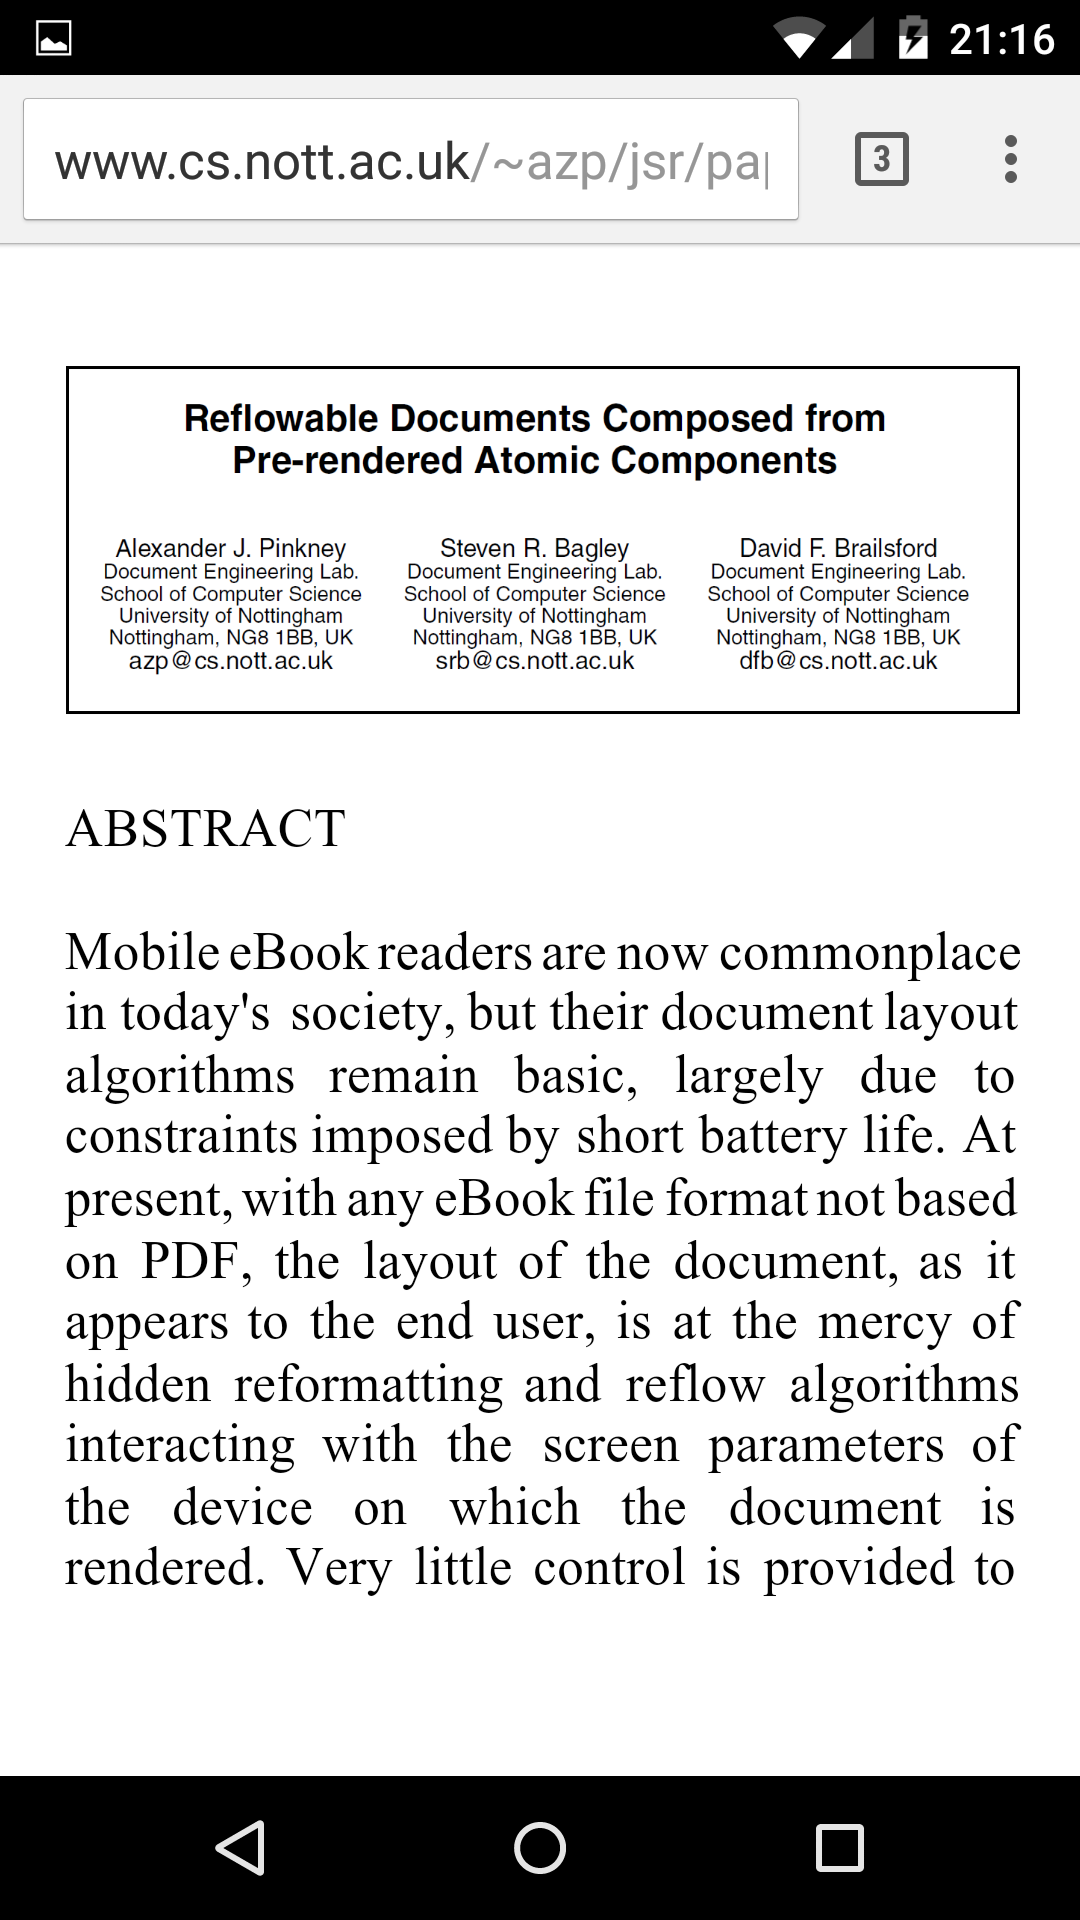
\includegraphics[width=\imgwid]{gfx/n5_p_1}}
\fbox{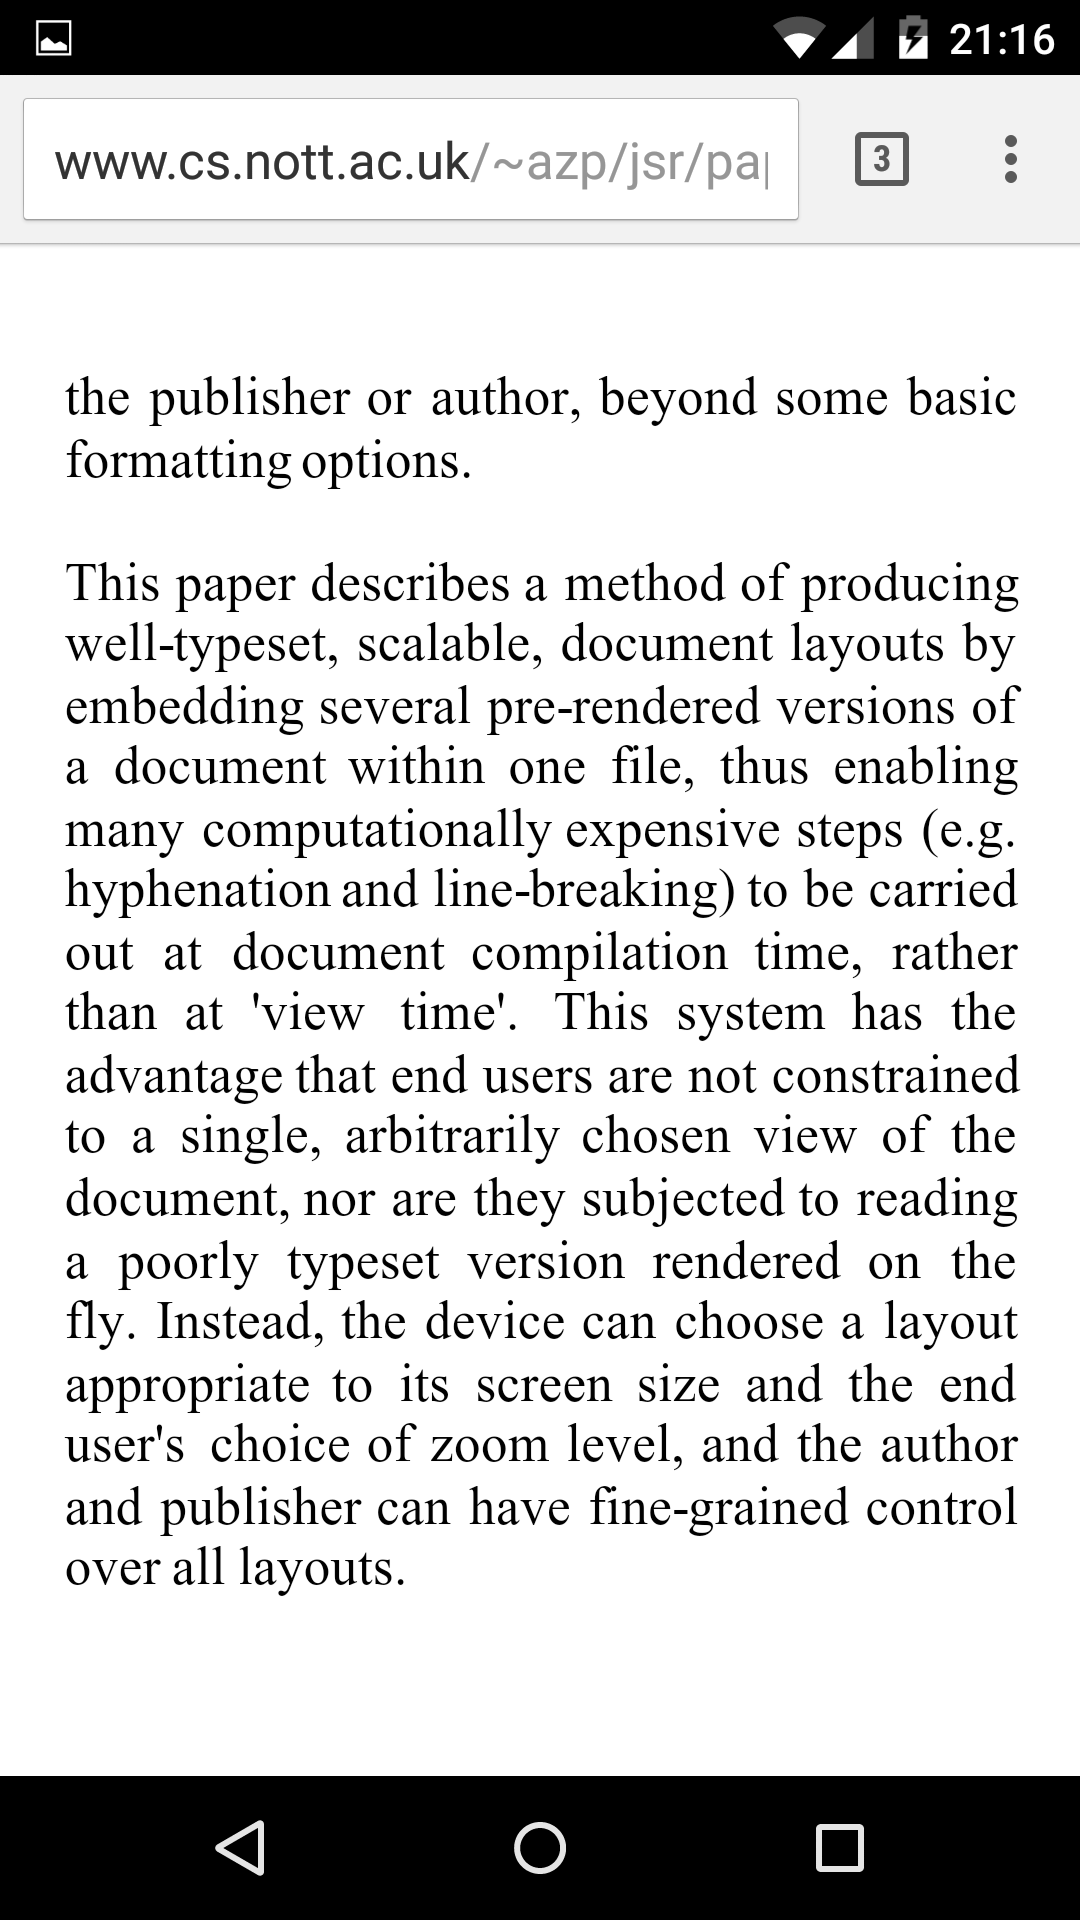
\includegraphics[width=\imgwid]{gfx/n5_p_2}}
\fbox{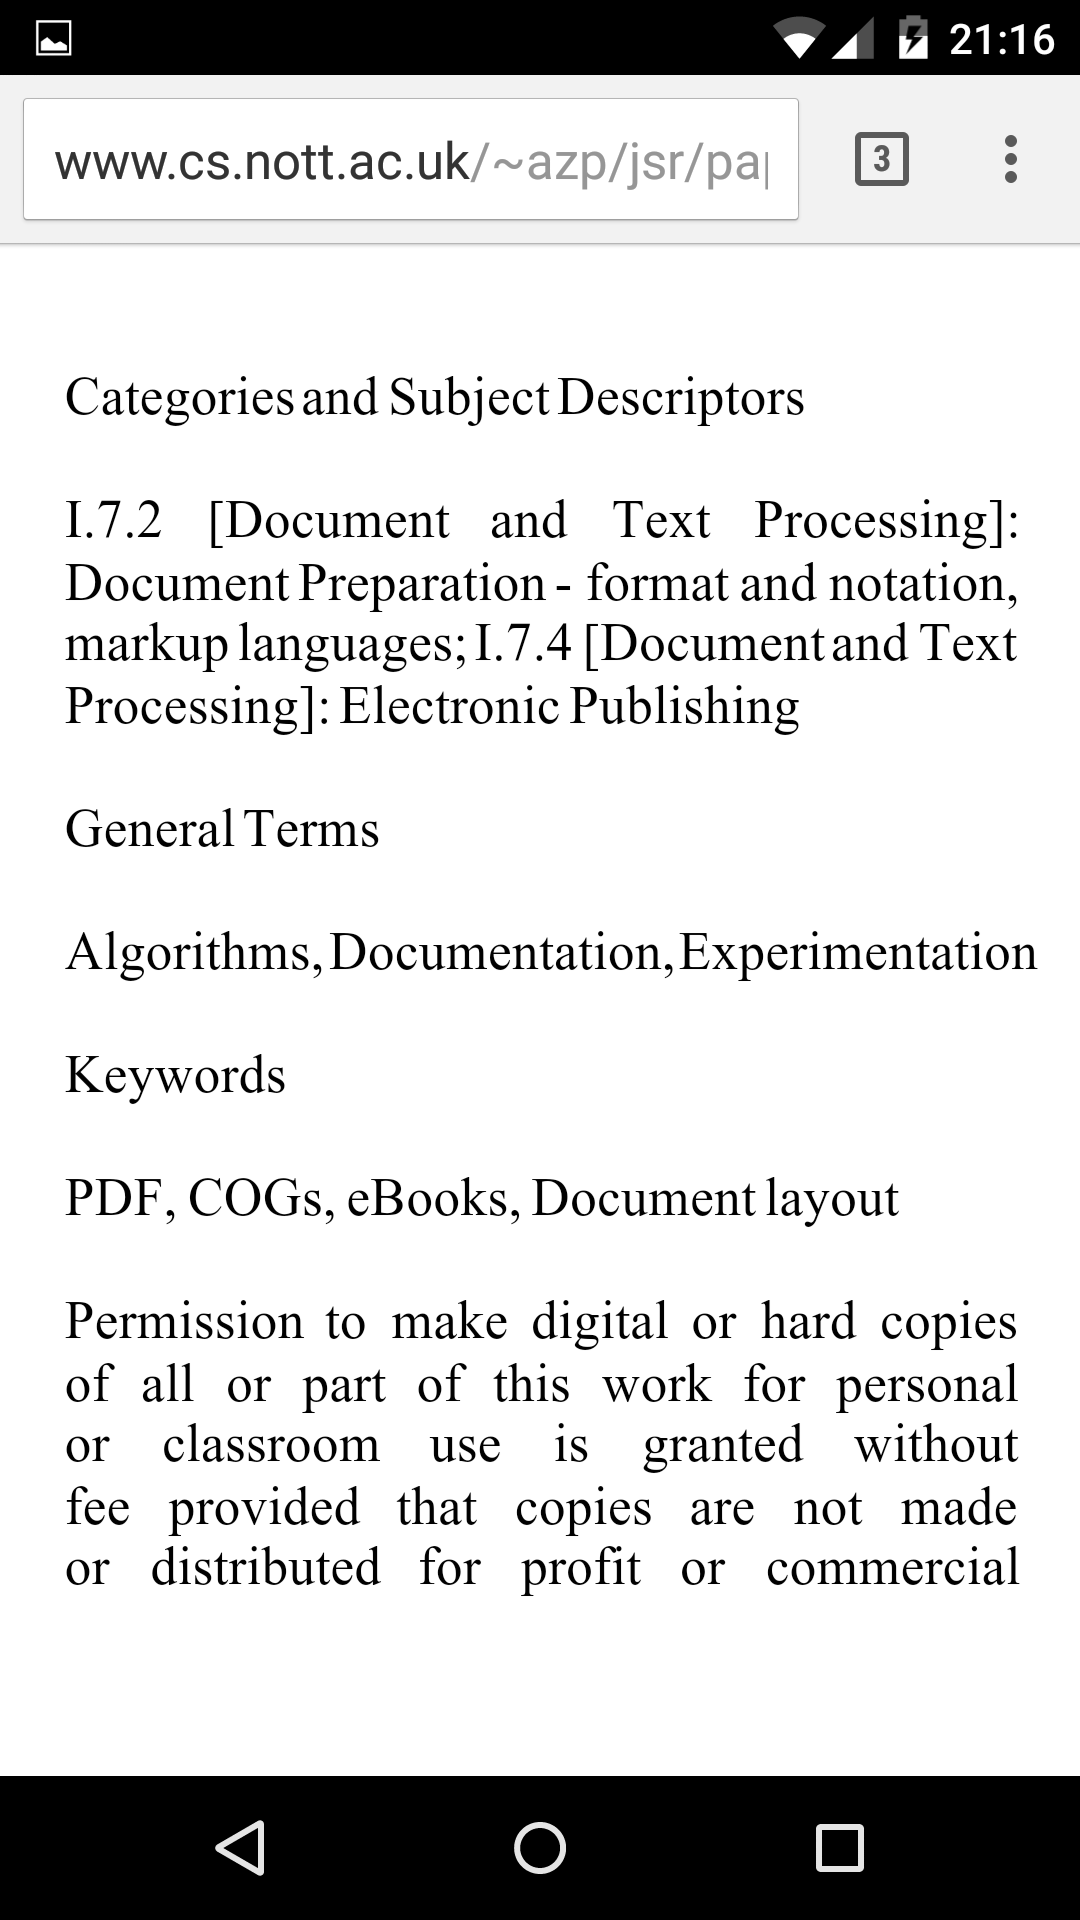
\includegraphics[width=\imgwid]{gfx/n5_p_3}}

\vspace{2em}

\fbox{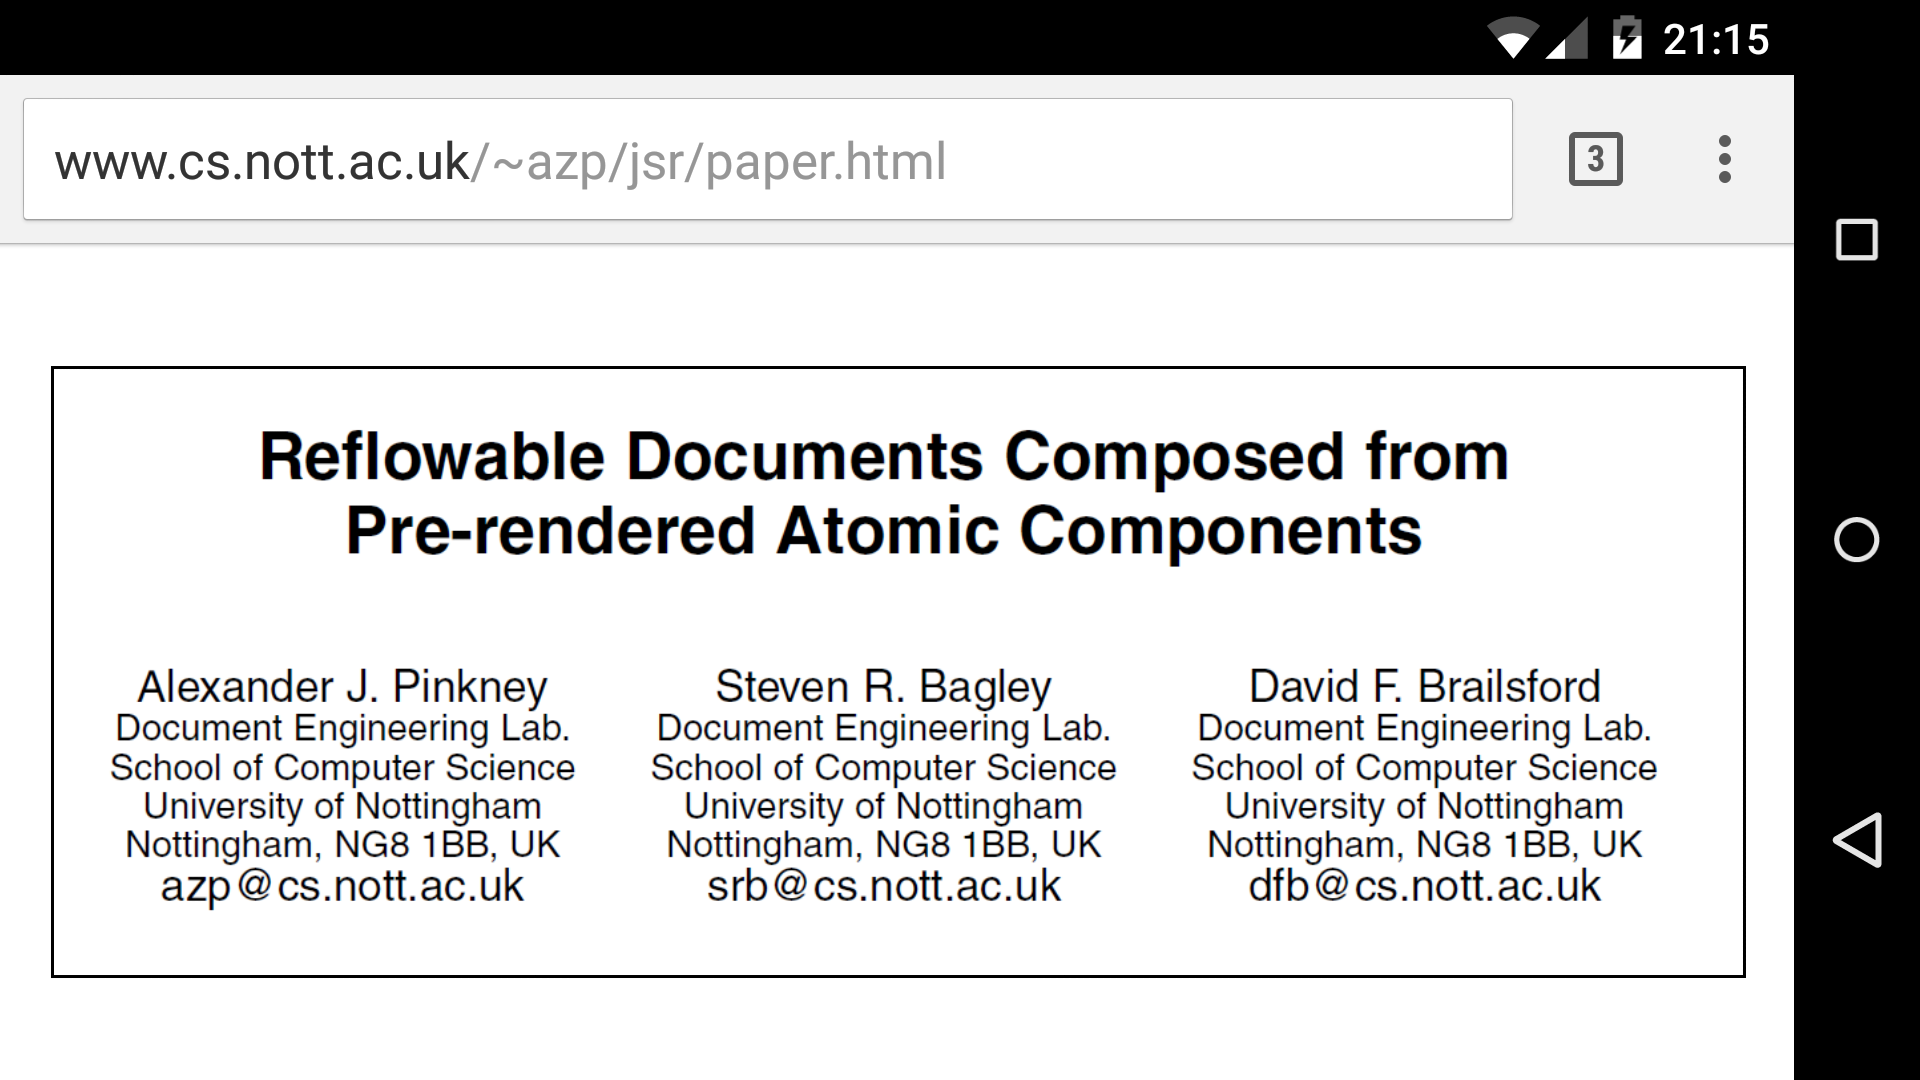
\includegraphics[height=\imgwid]{gfx/n5_l_1}}
\fbox{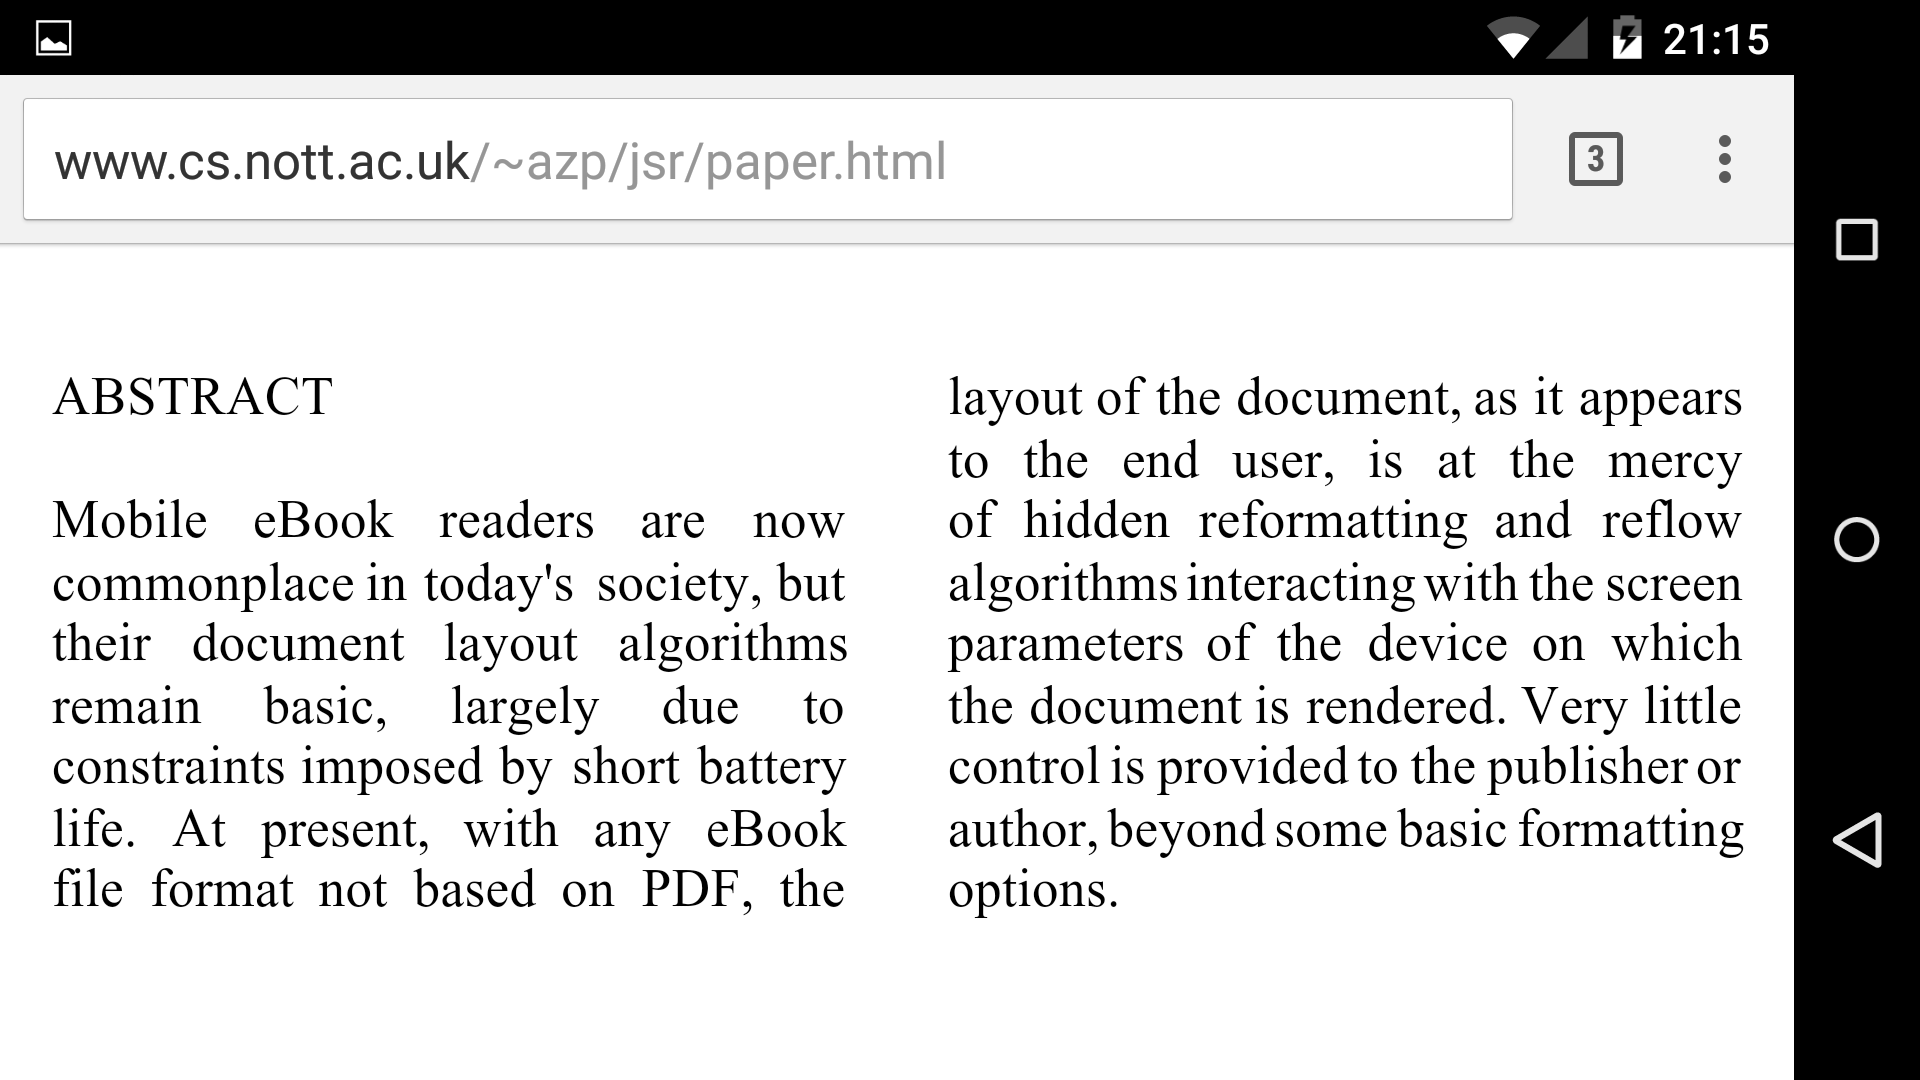
\includegraphics[height=\imgwid]{gfx/n5_l_2}}
\fbox{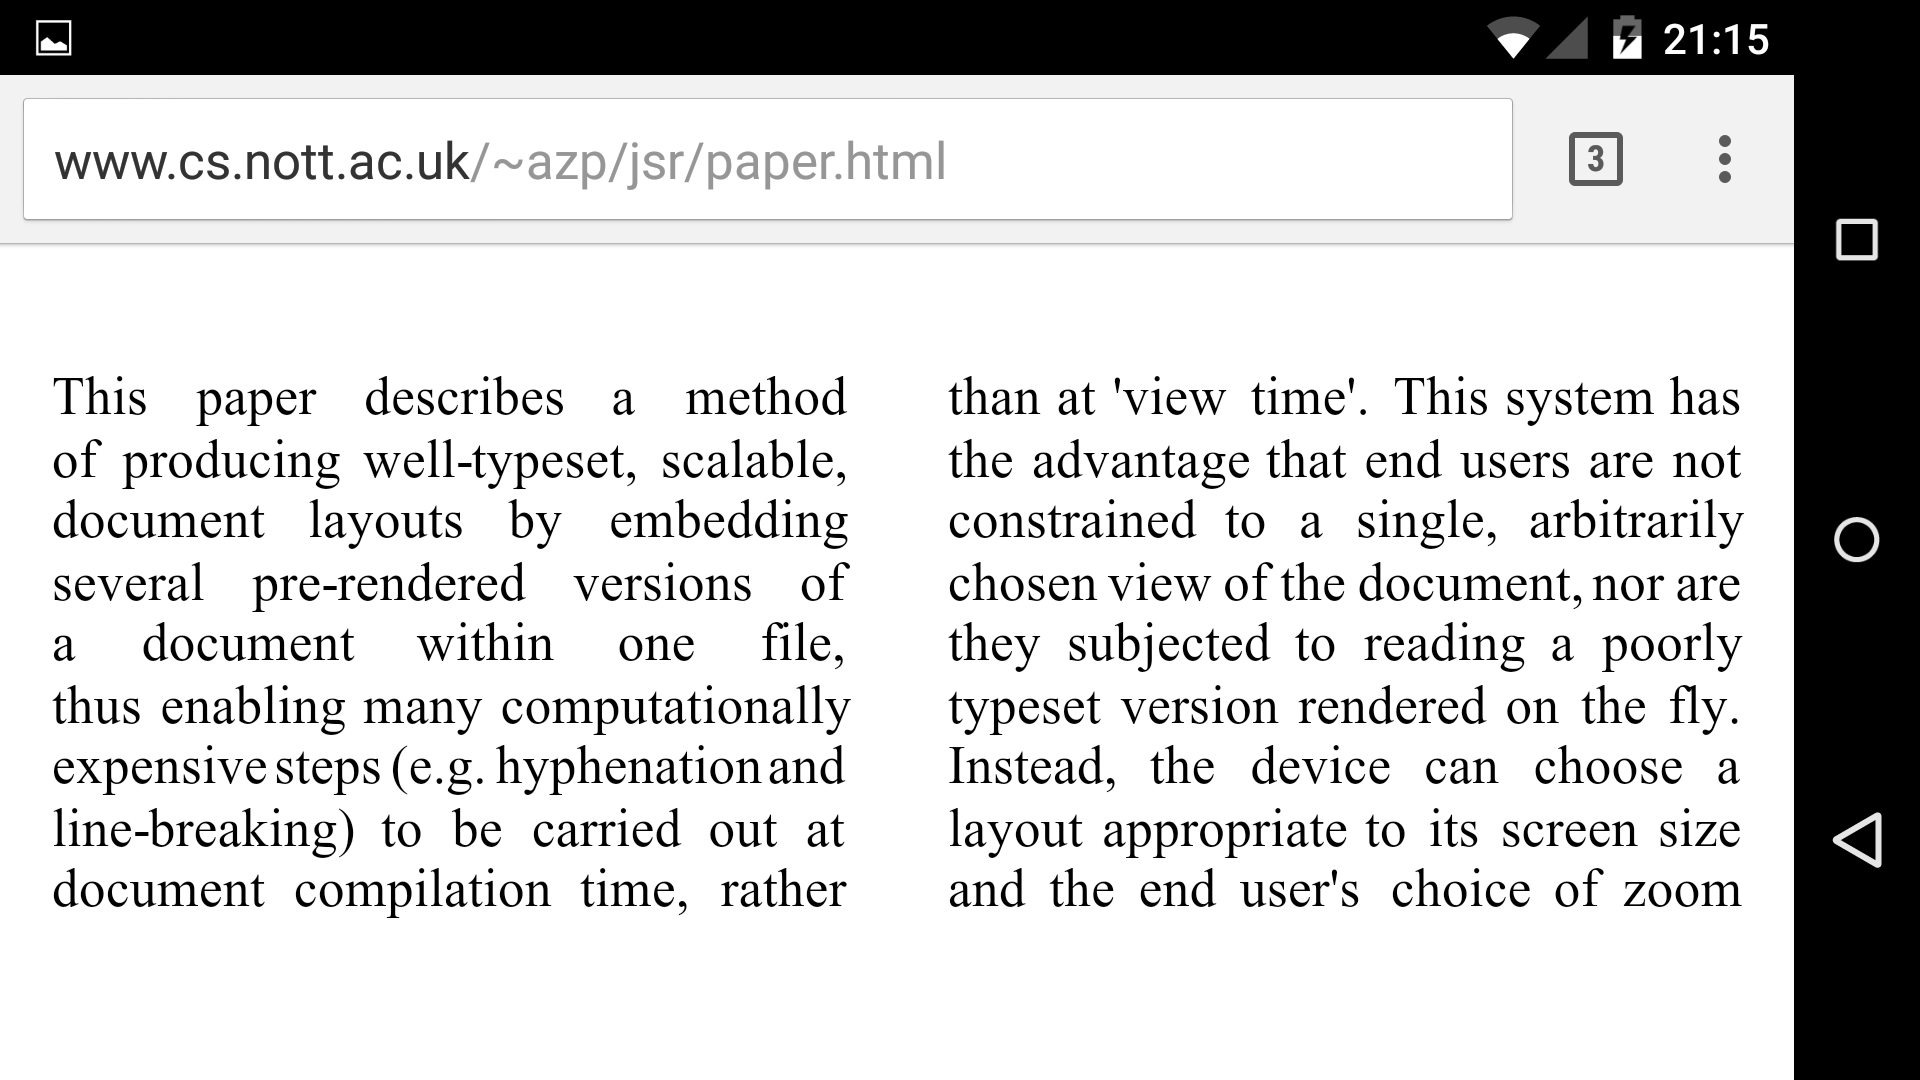
\includegraphics[height=\imgwid]{gfx/n5_l_3}}
\end{center}


\clearpage


\subsection{Safari on an iPad}
\label{app:layout-ipad}

\cite{Pinkney2011} rendered in Safari on a iPad in portrait orientation:
\begin{center}
\setlength{\imgwid}{0.47\textwidth}
\fbox{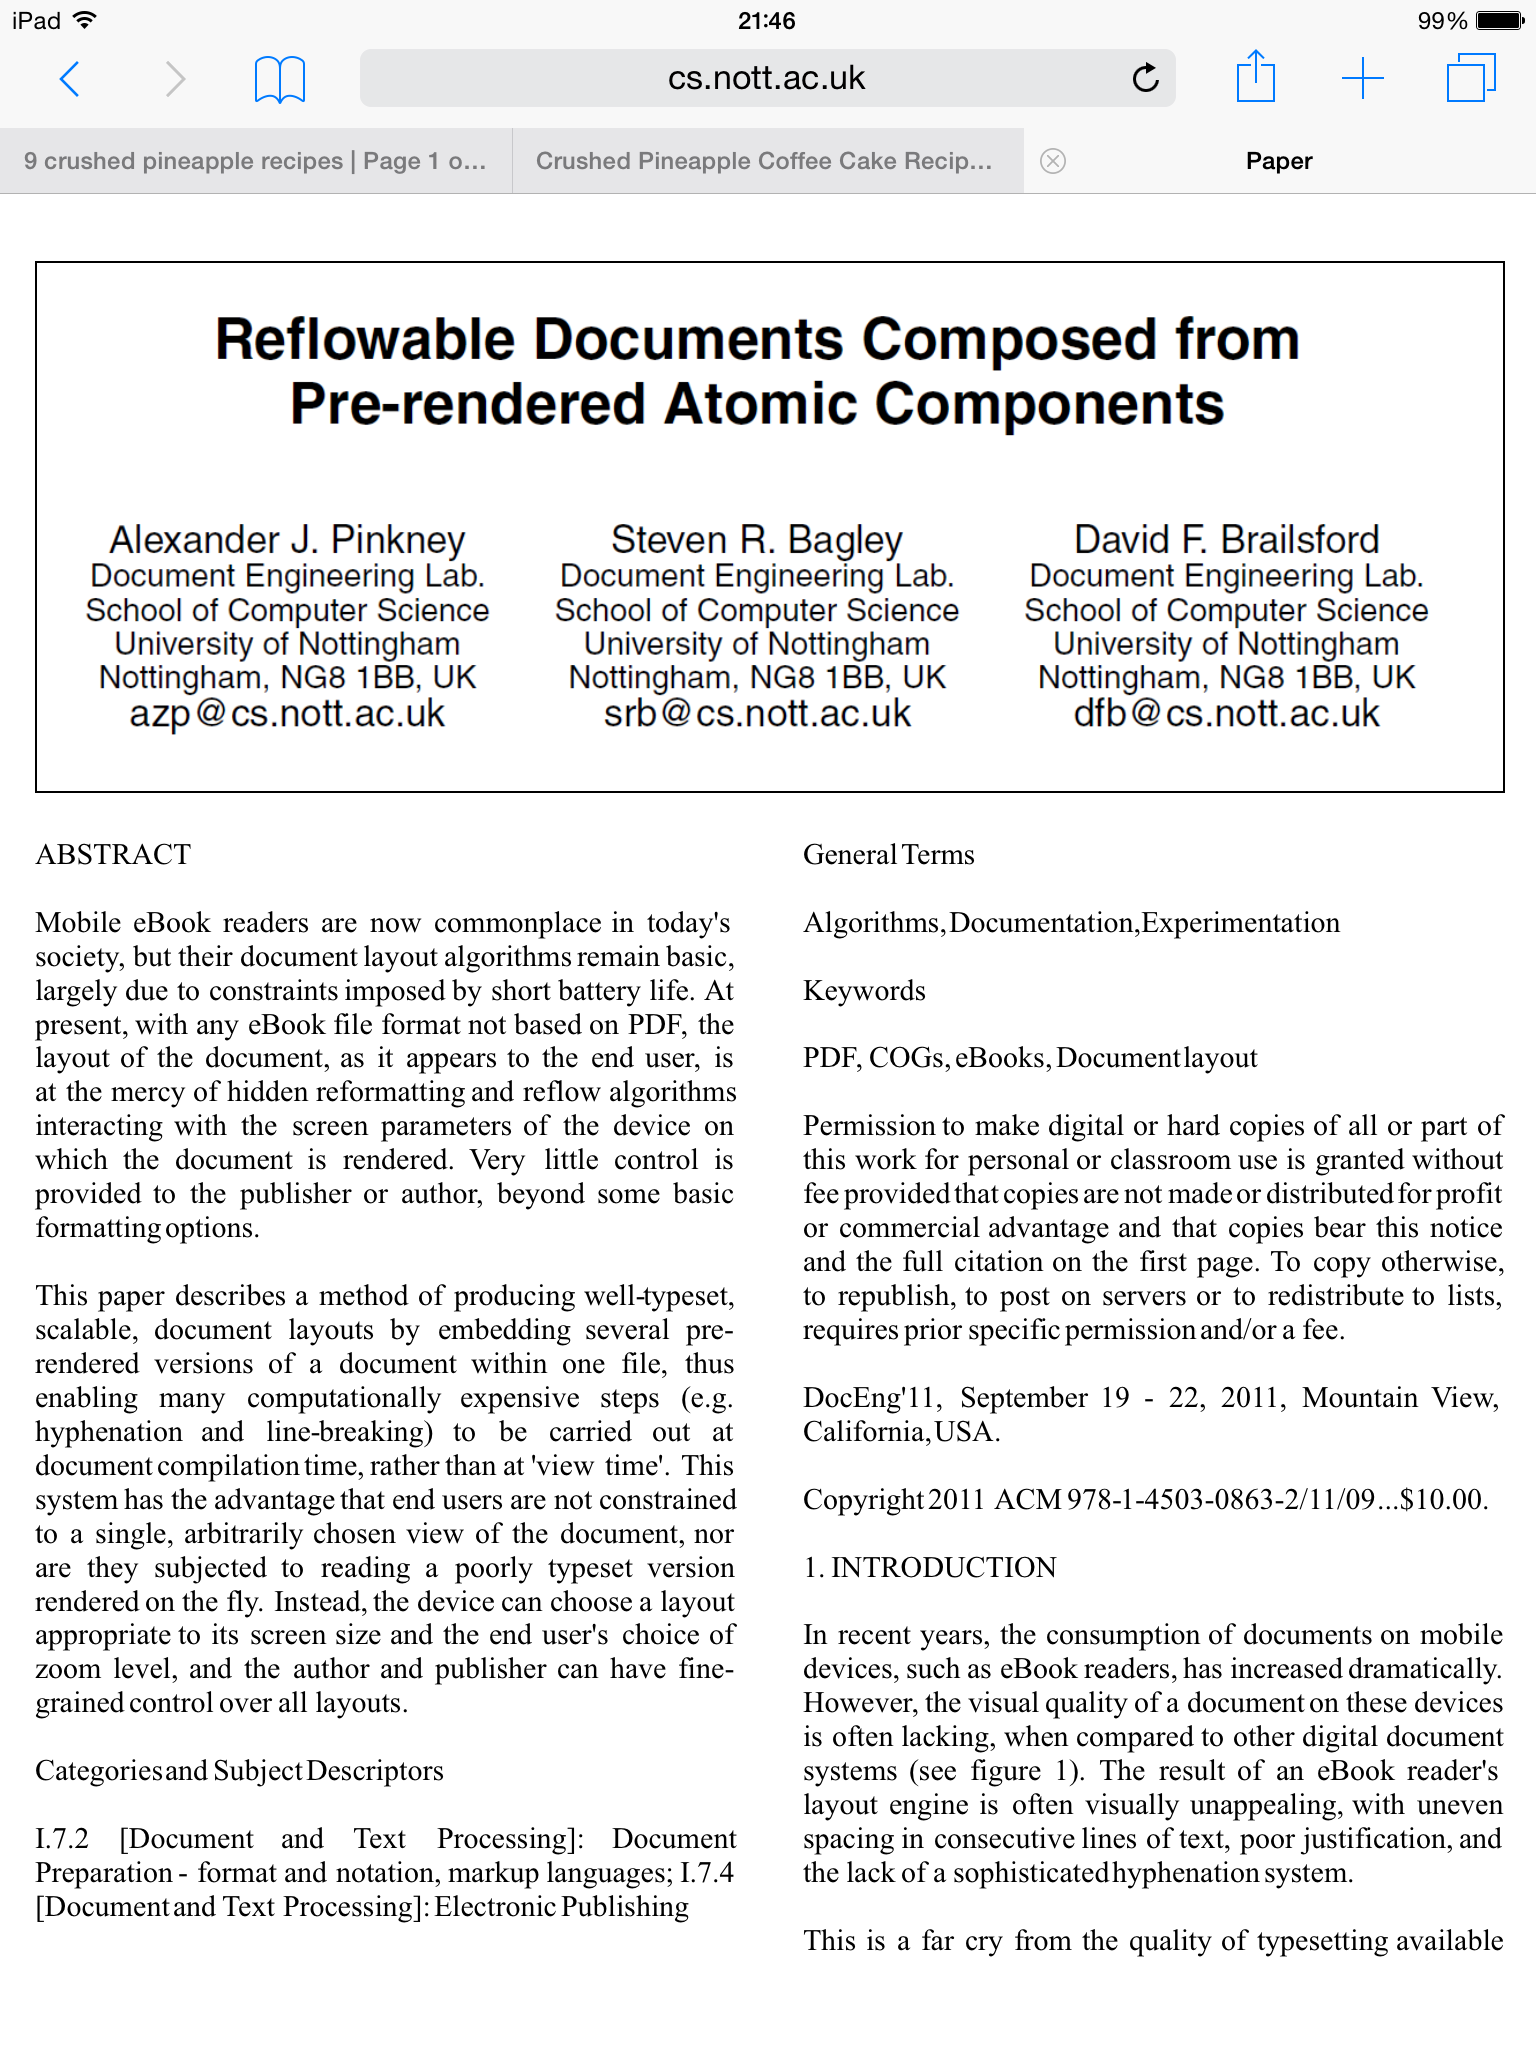
\includegraphics[width=\imgwid]{gfx/ipad-p1}}
\fbox{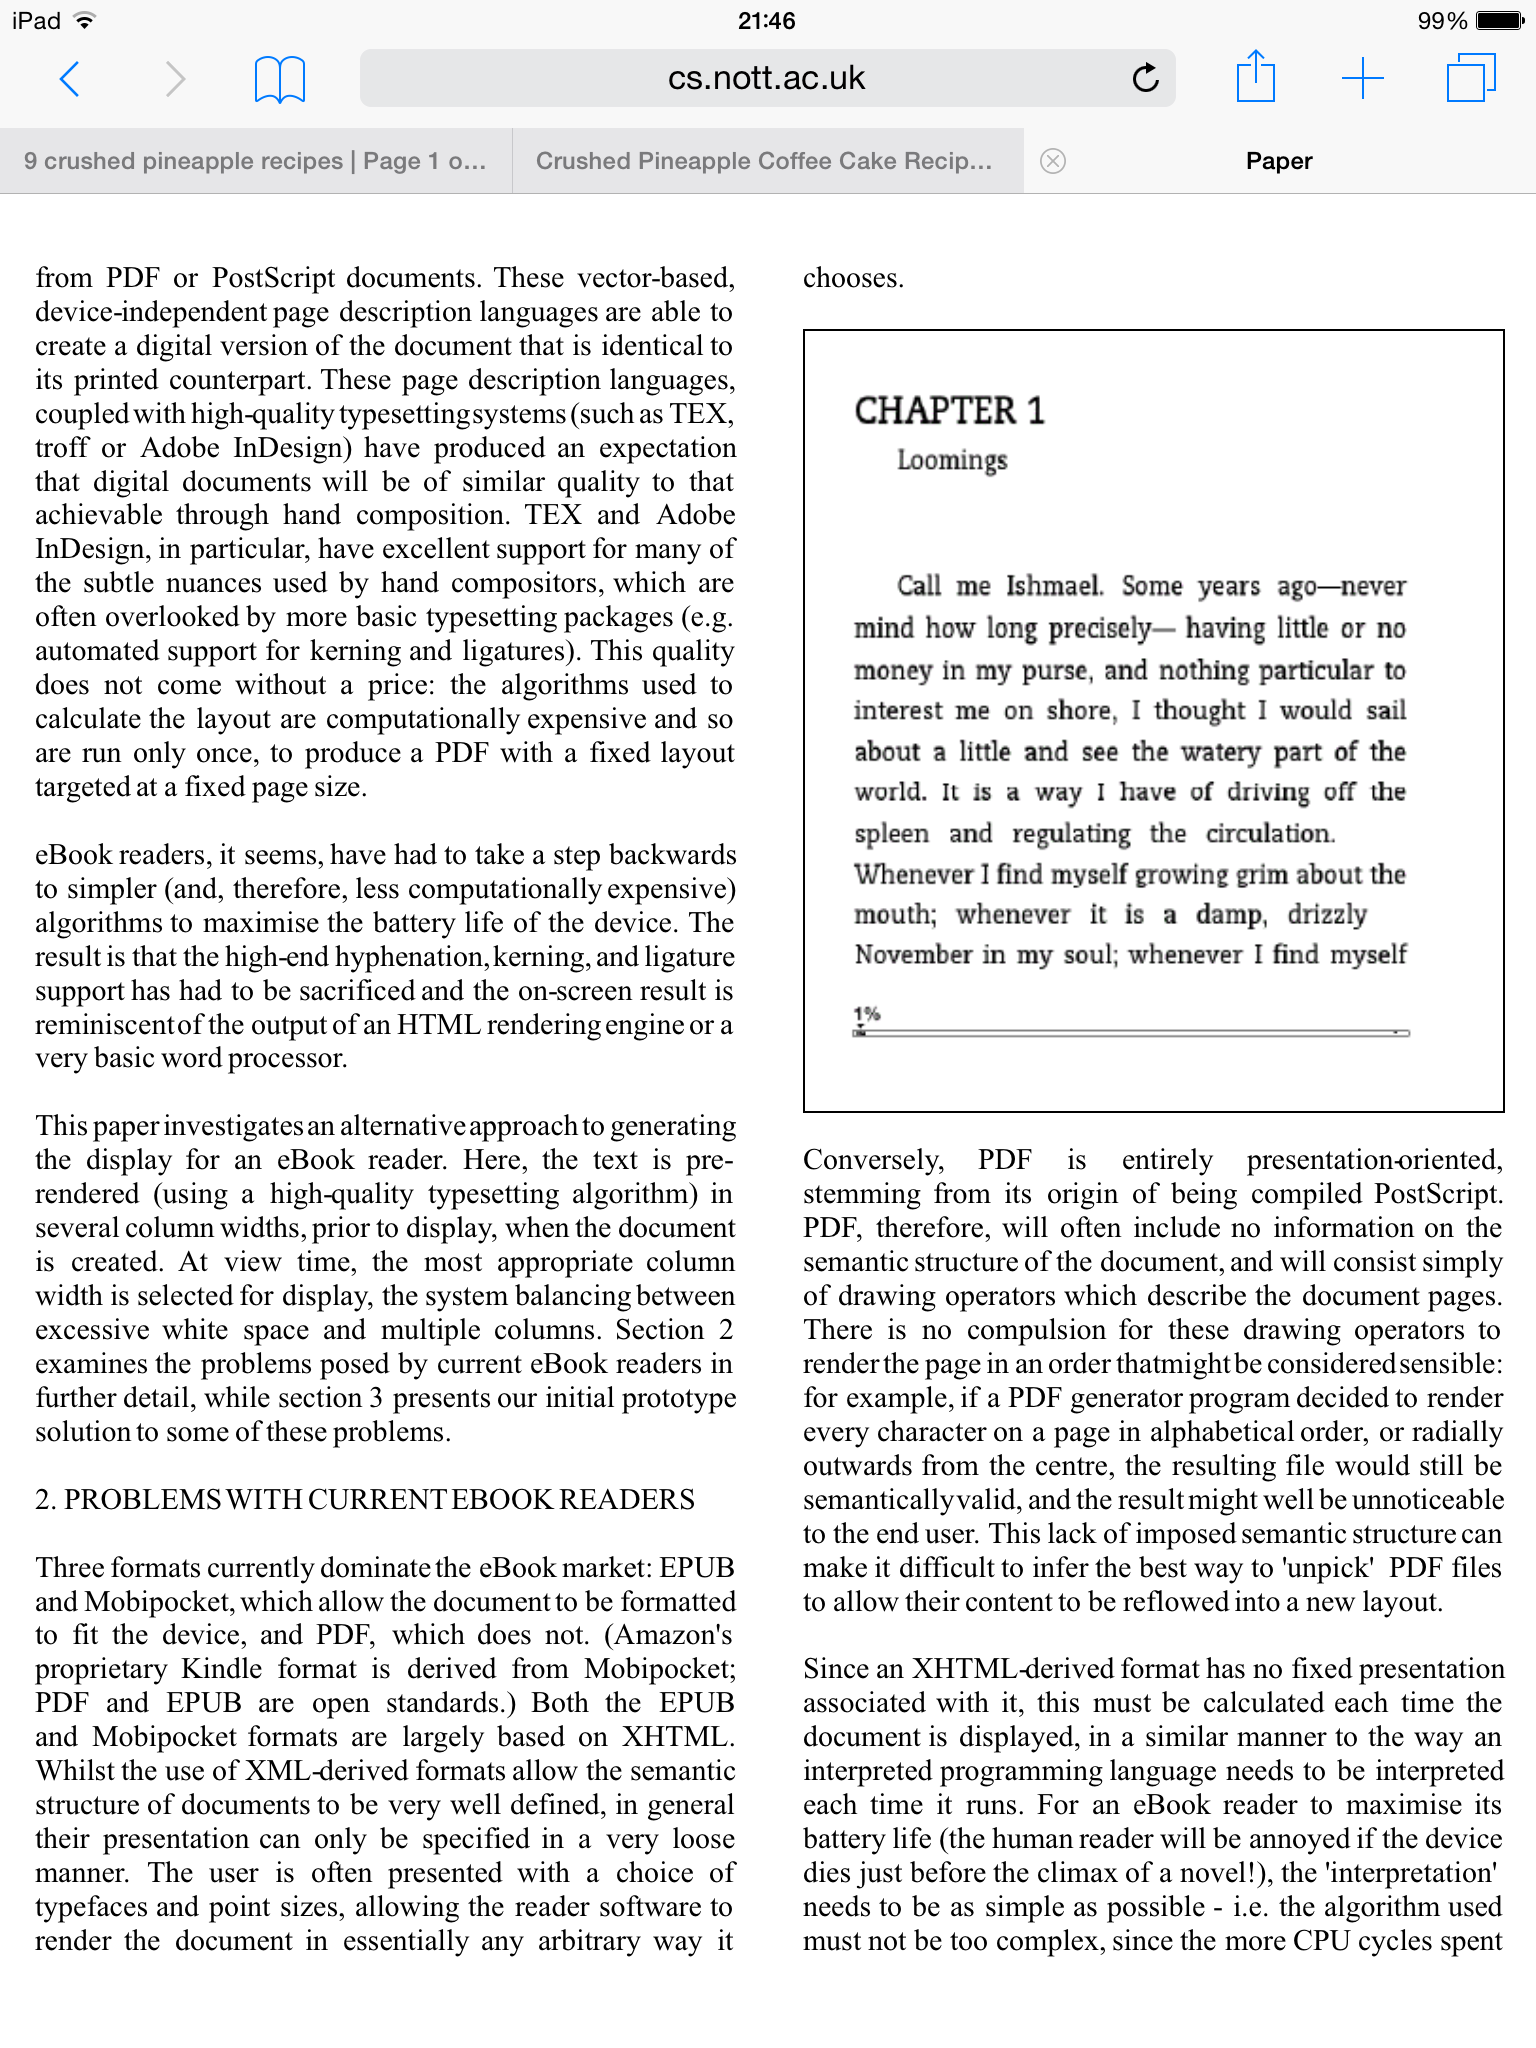
\includegraphics[width=\imgwid]{gfx/ipad-p2}}

\vspace{0.3em}

\fbox{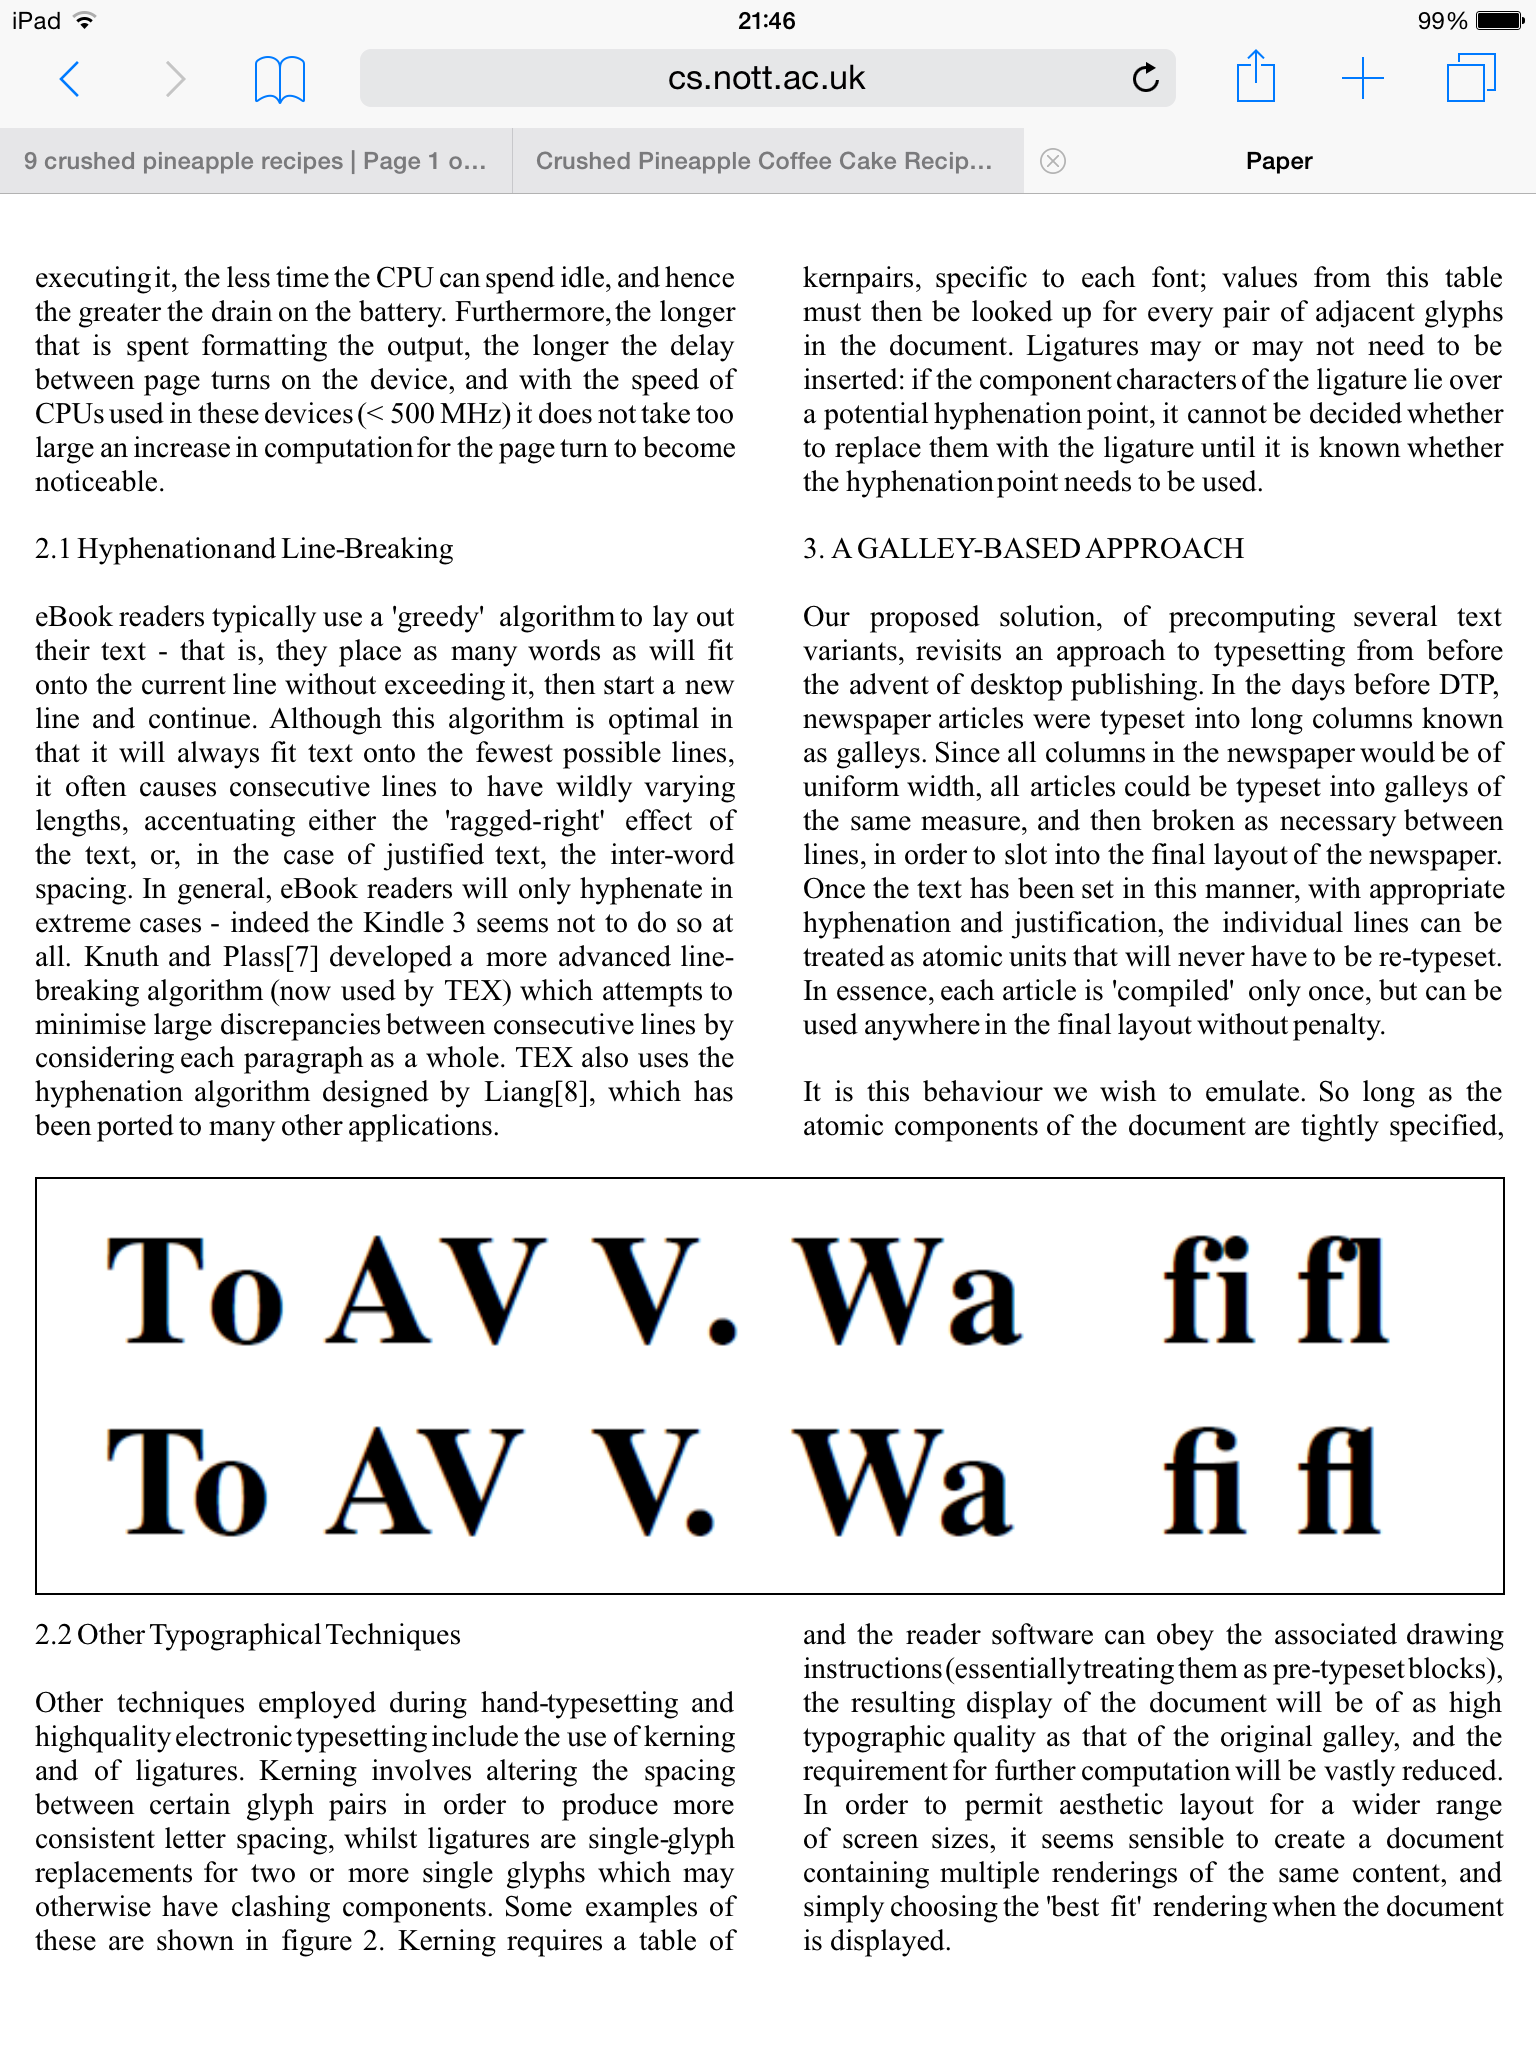
\includegraphics[width=\imgwid]{gfx/ipad-p3}}
\fbox{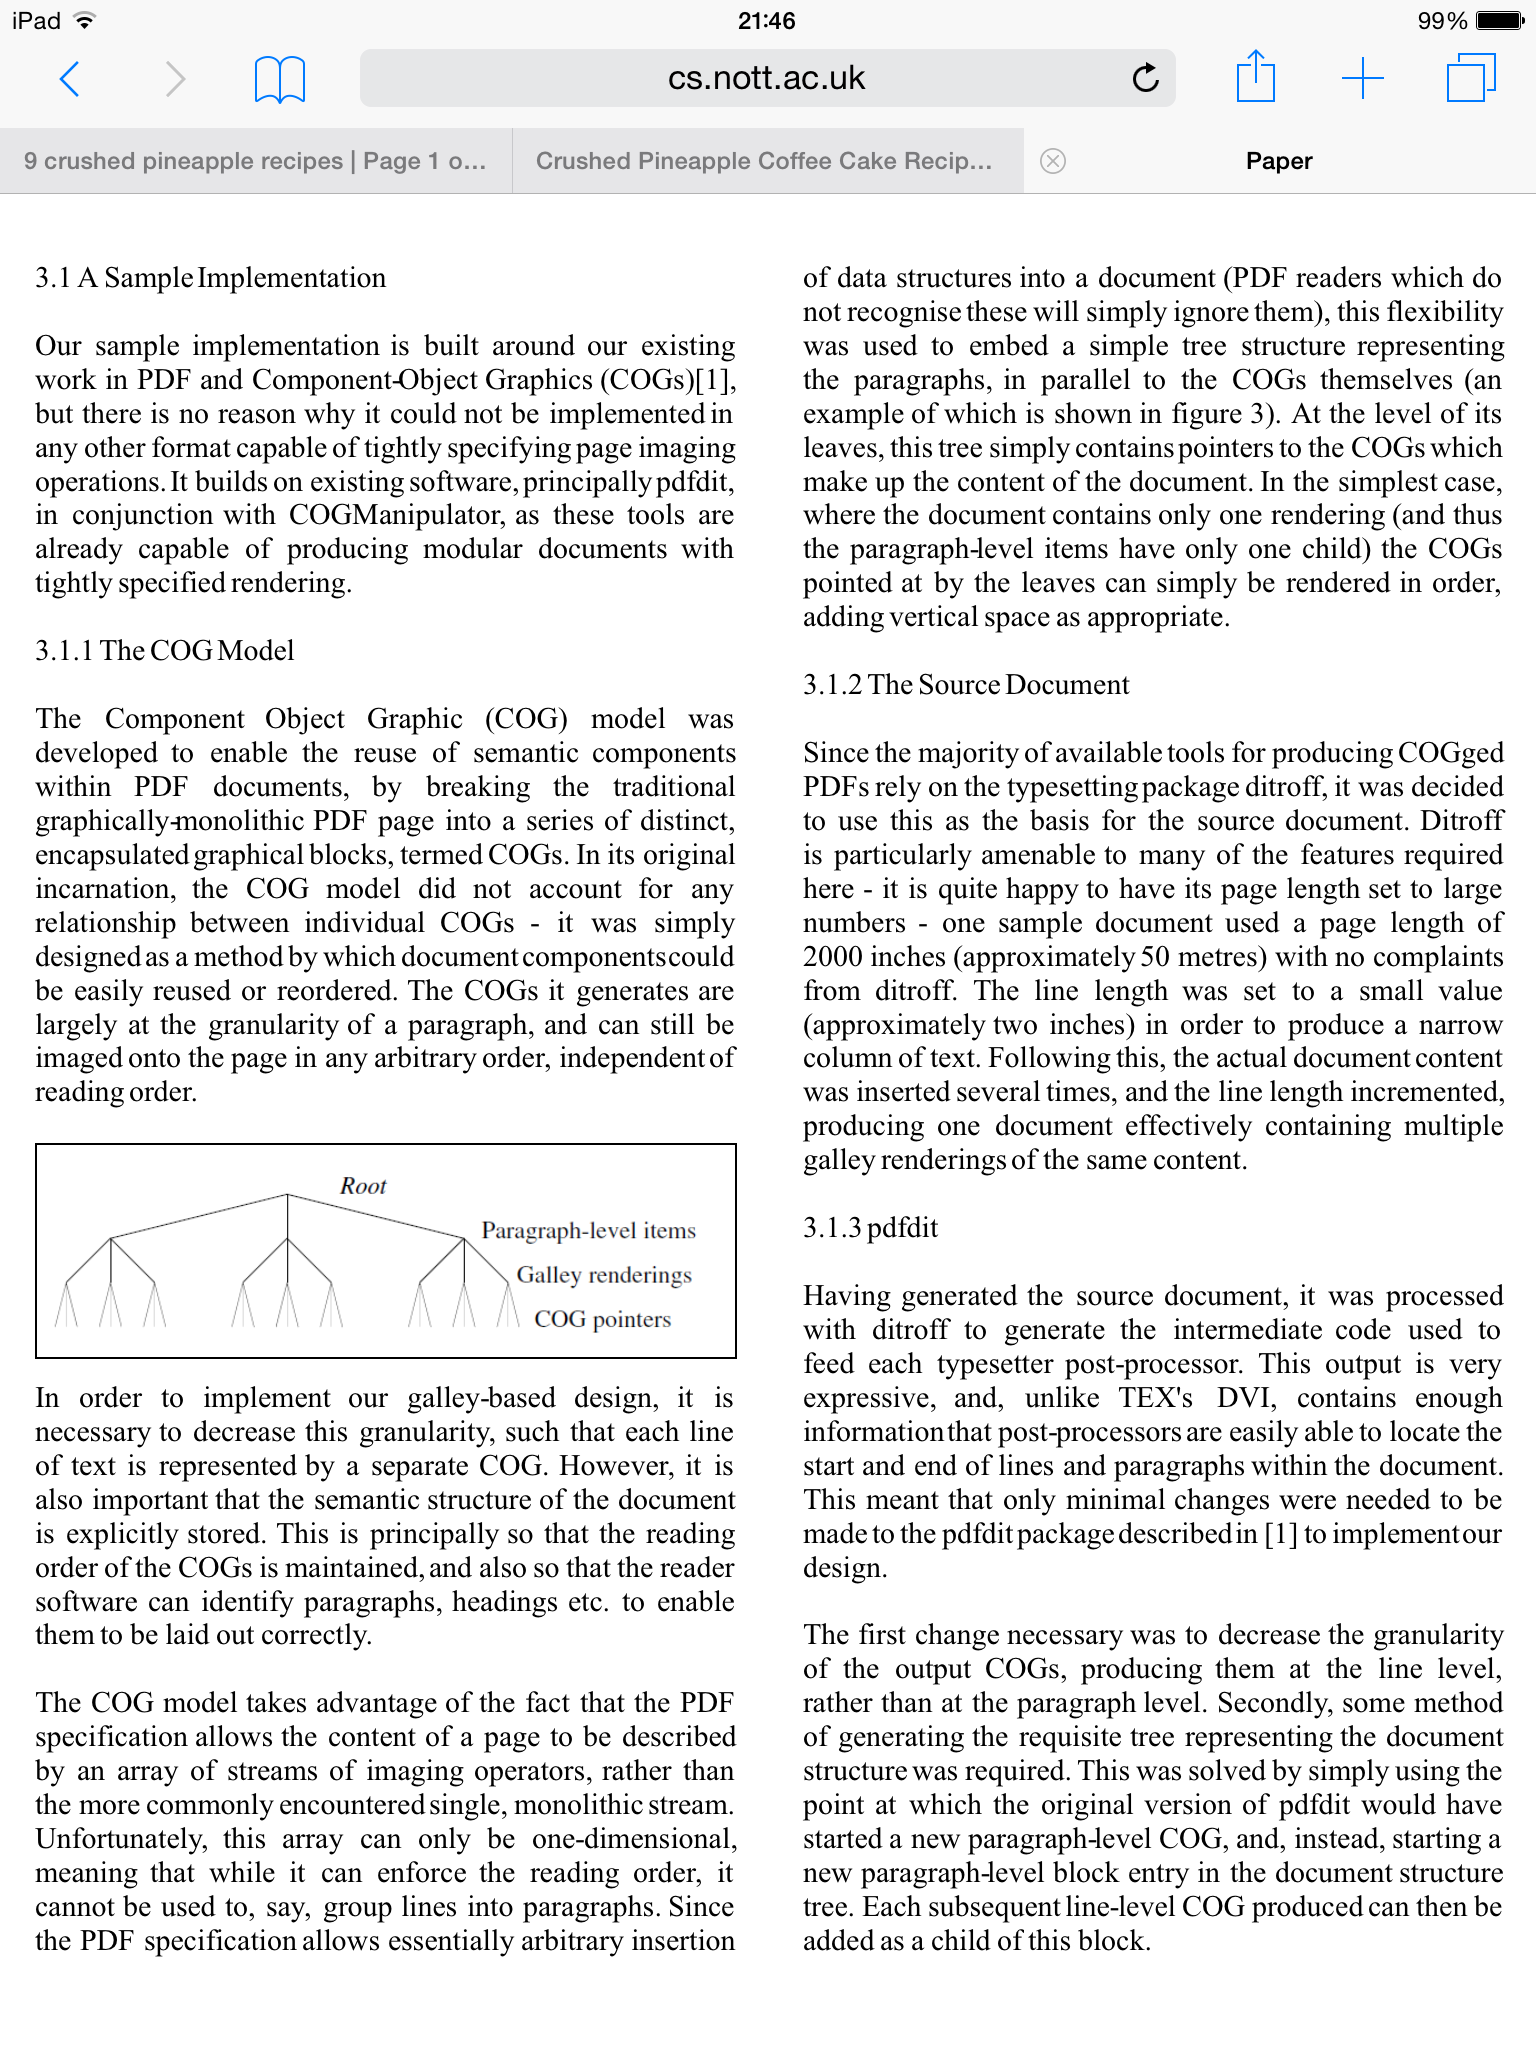
\includegraphics[width=\imgwid]{gfx/ipad-p4}}

\end{center}

\clearpage
\cite{Pinkney2011} rendered in Safari on a iPad in landscape orientation:
\begin{center}
\setlength{\imgwid}{0.8\textwidth}
\fbox{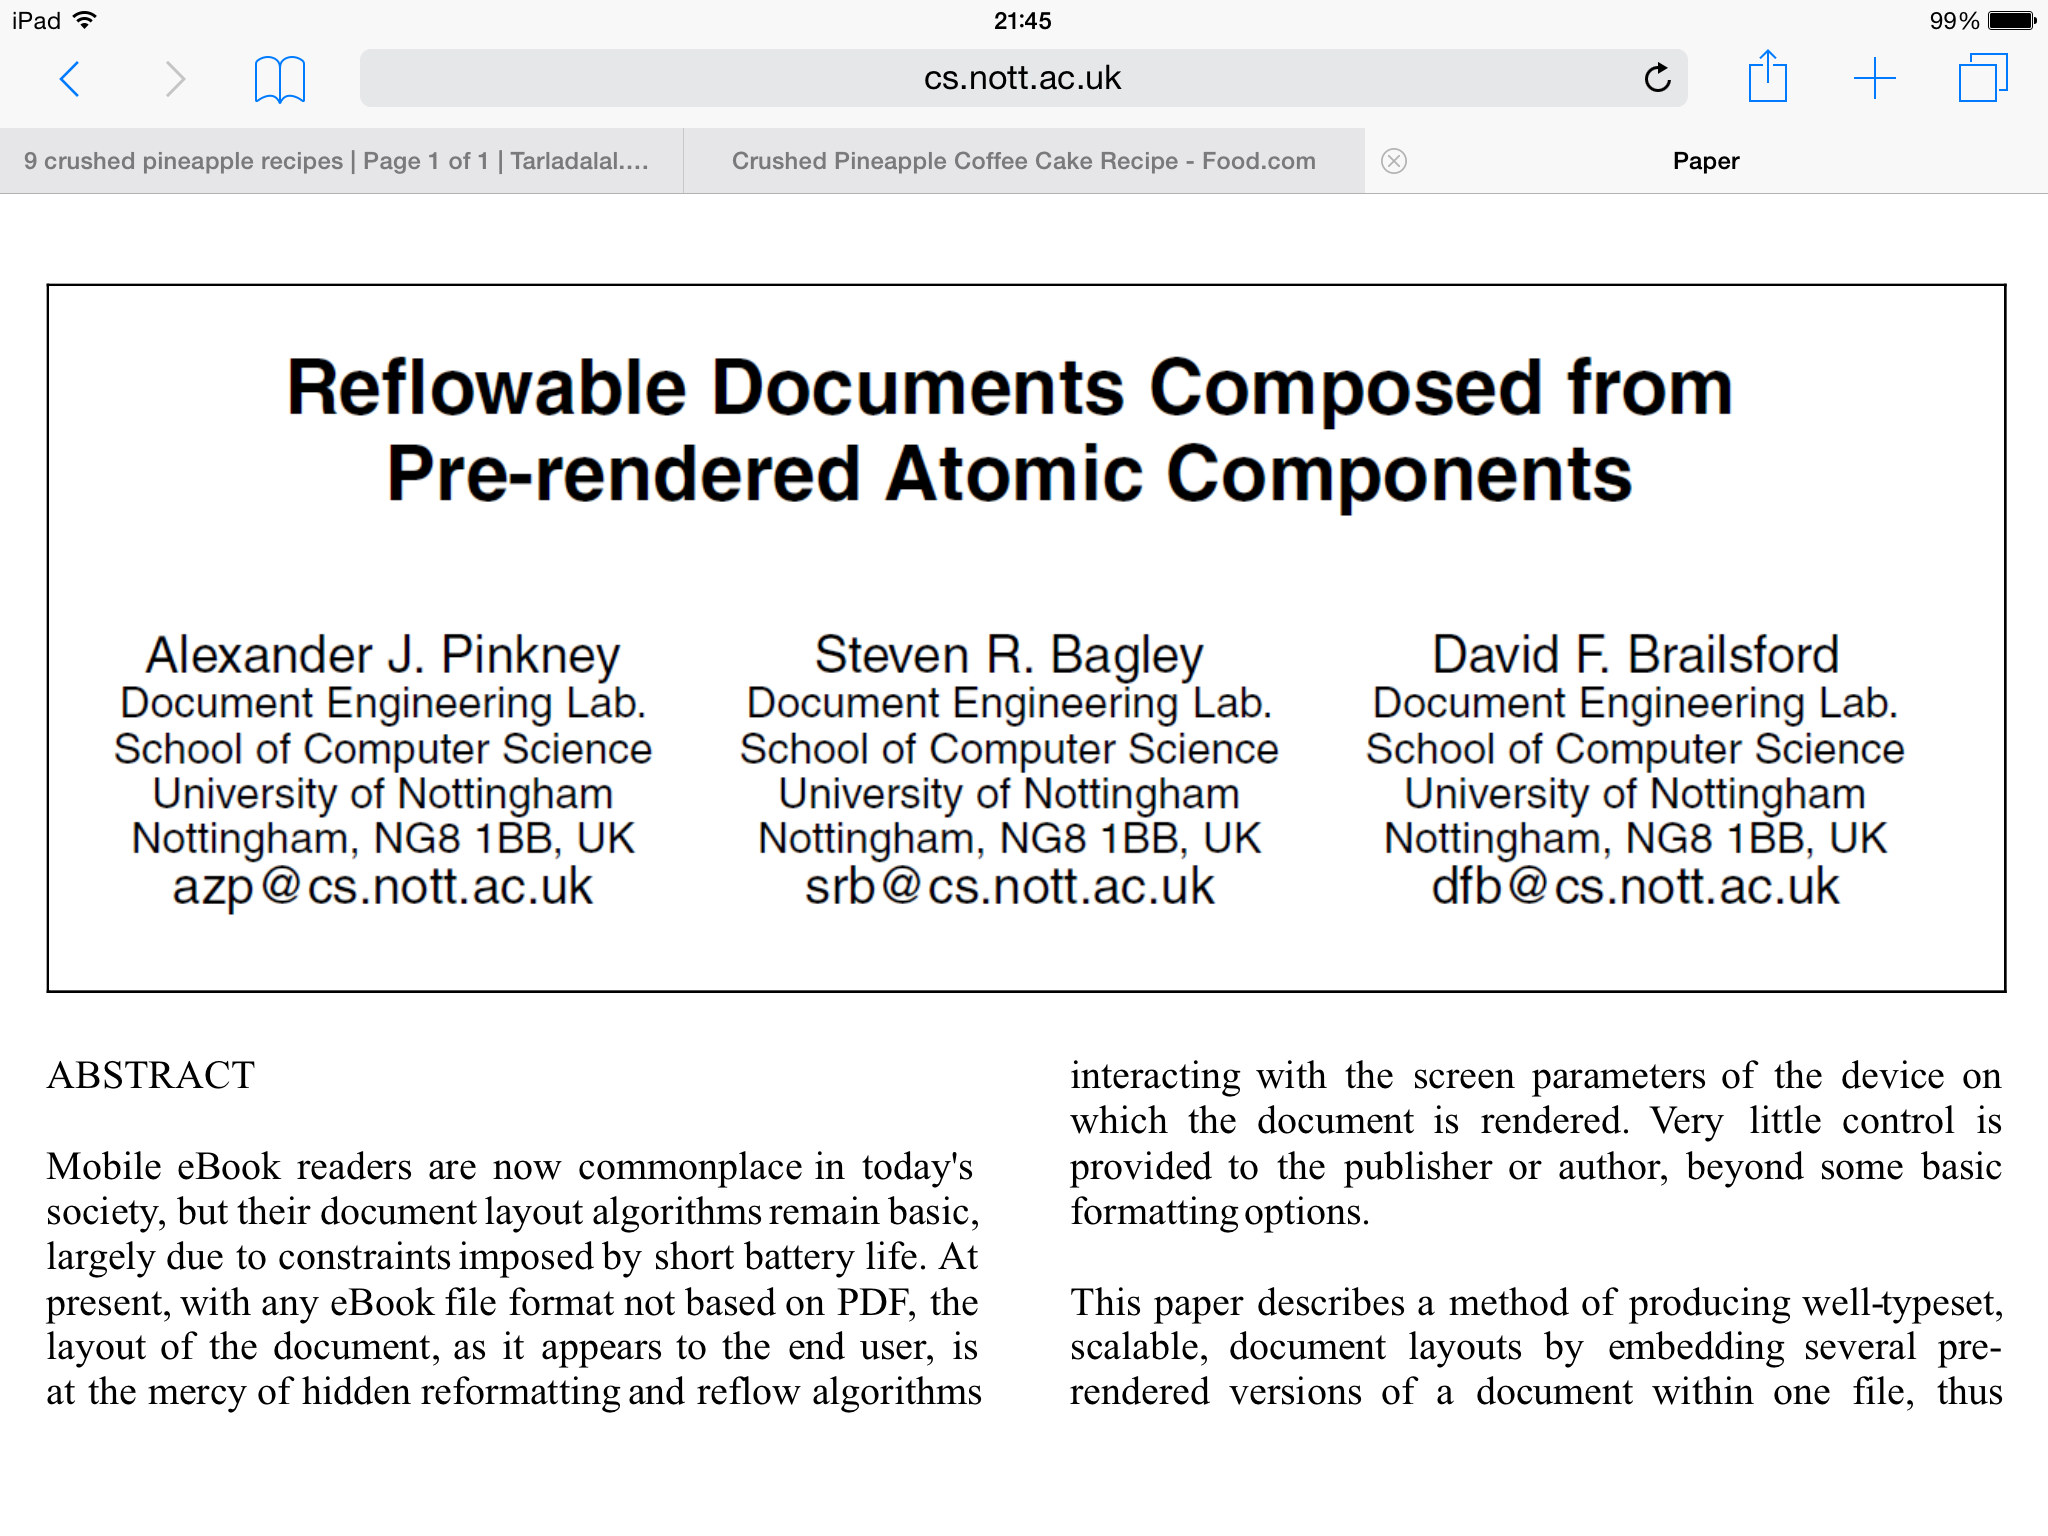
\includegraphics[width=\imgwid]{gfx/ipad-l1}}

\vspace{0.3em}

\fbox{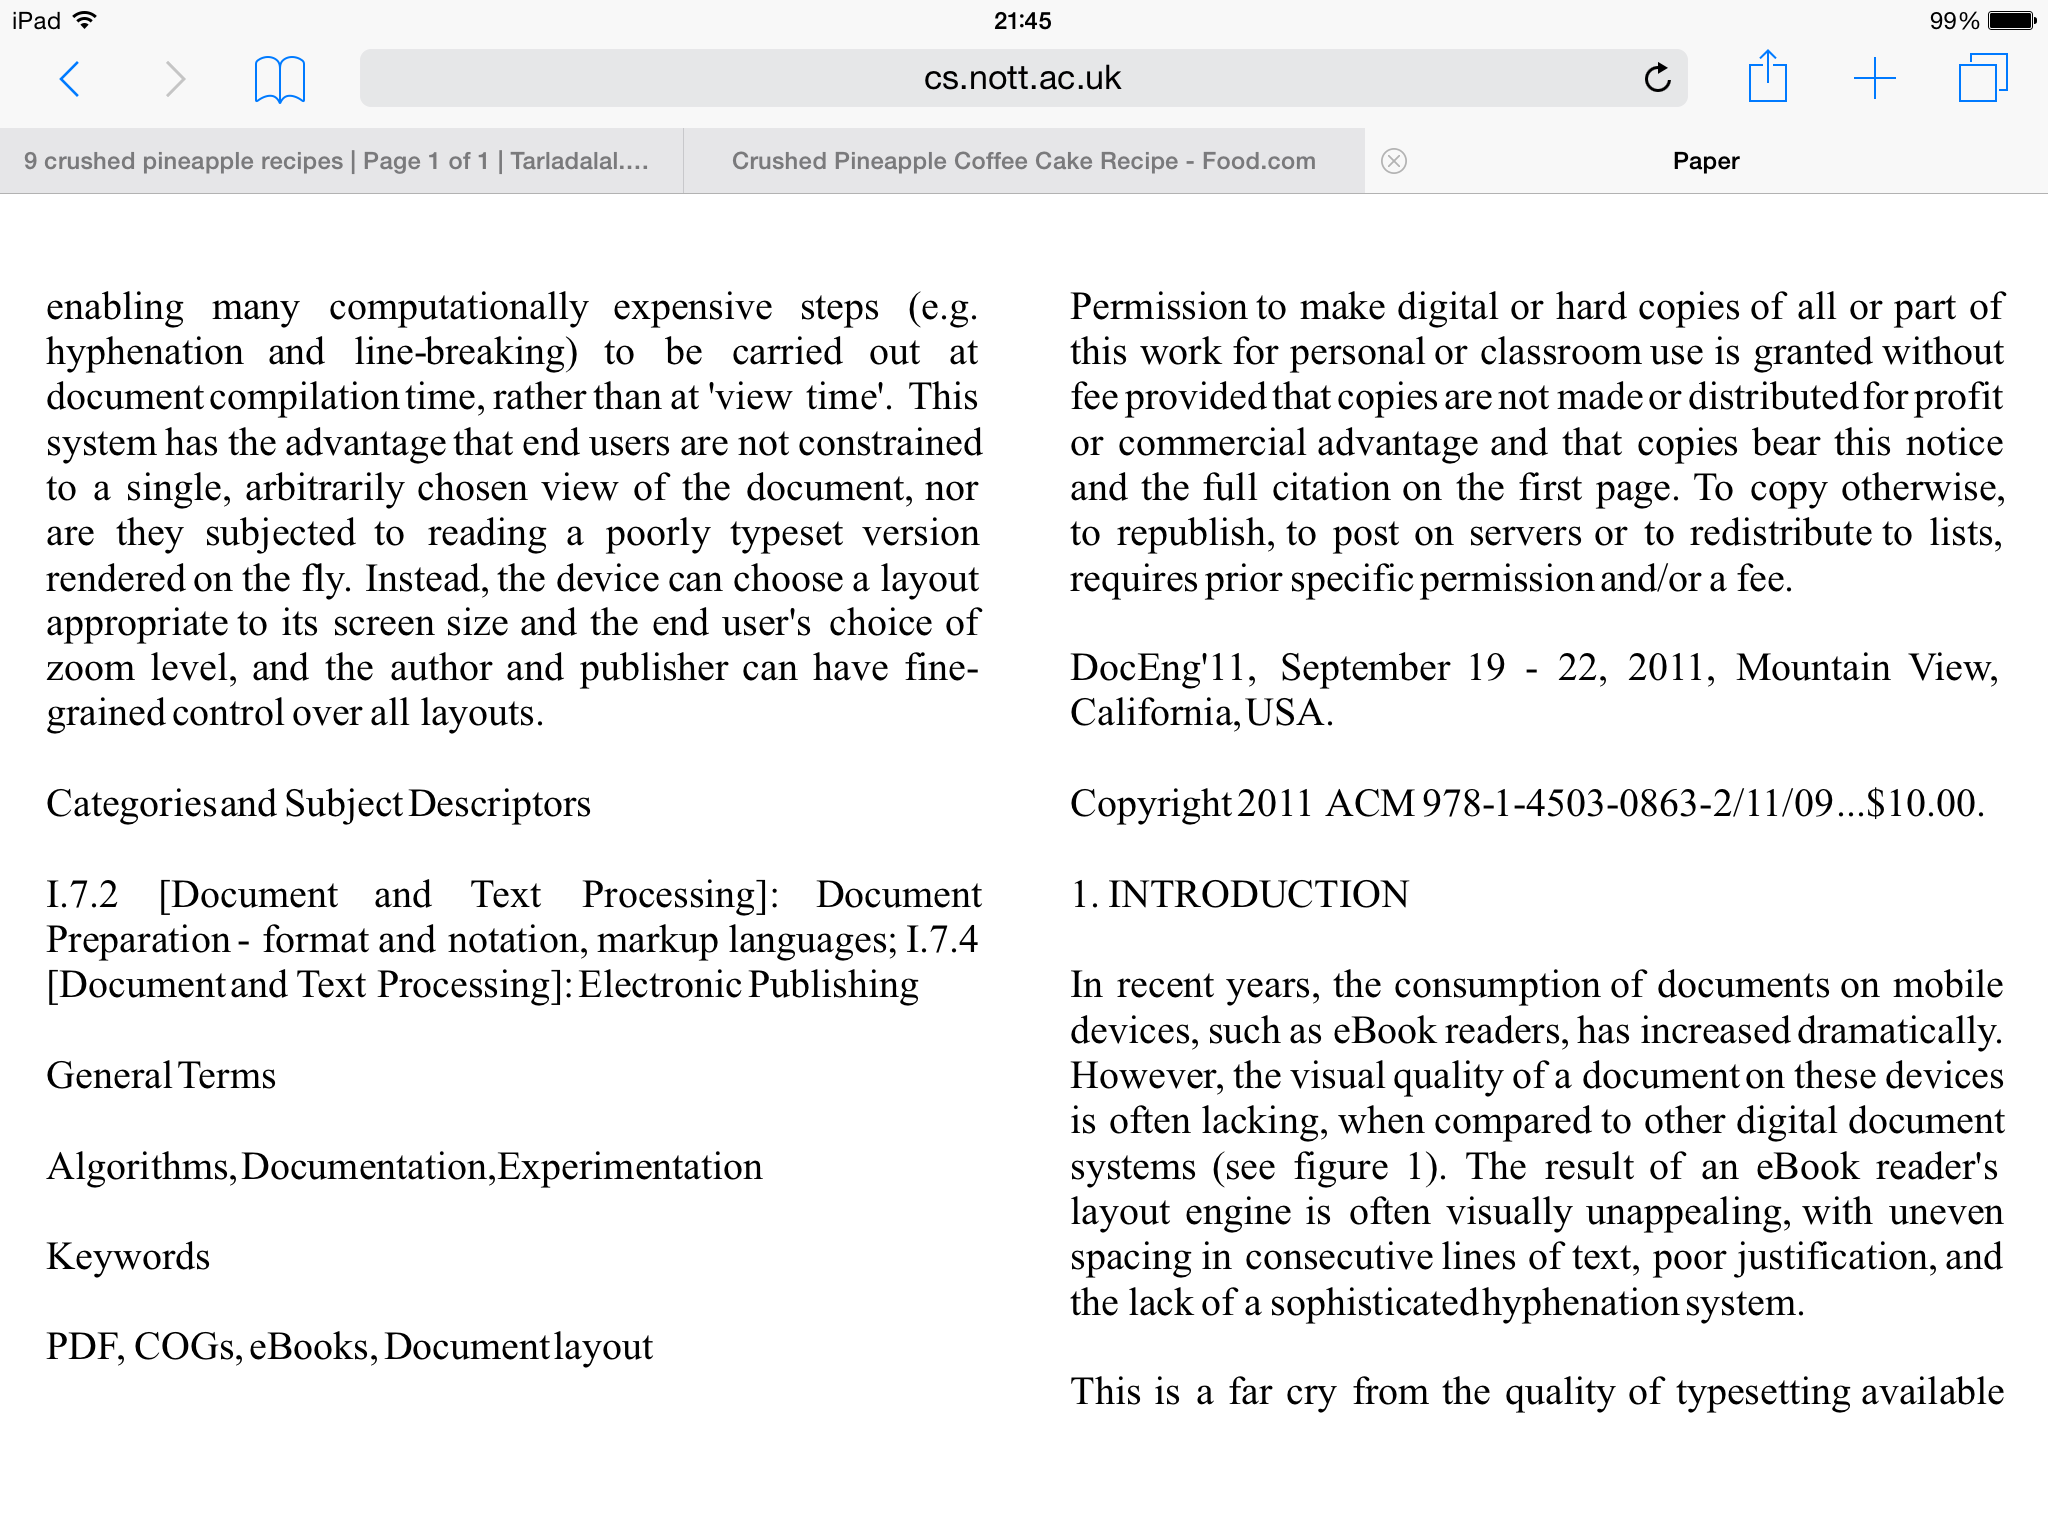
\includegraphics[width=\imgwid]{gfx/ipad-l2}}

\vspace{0.3em}

\fbox{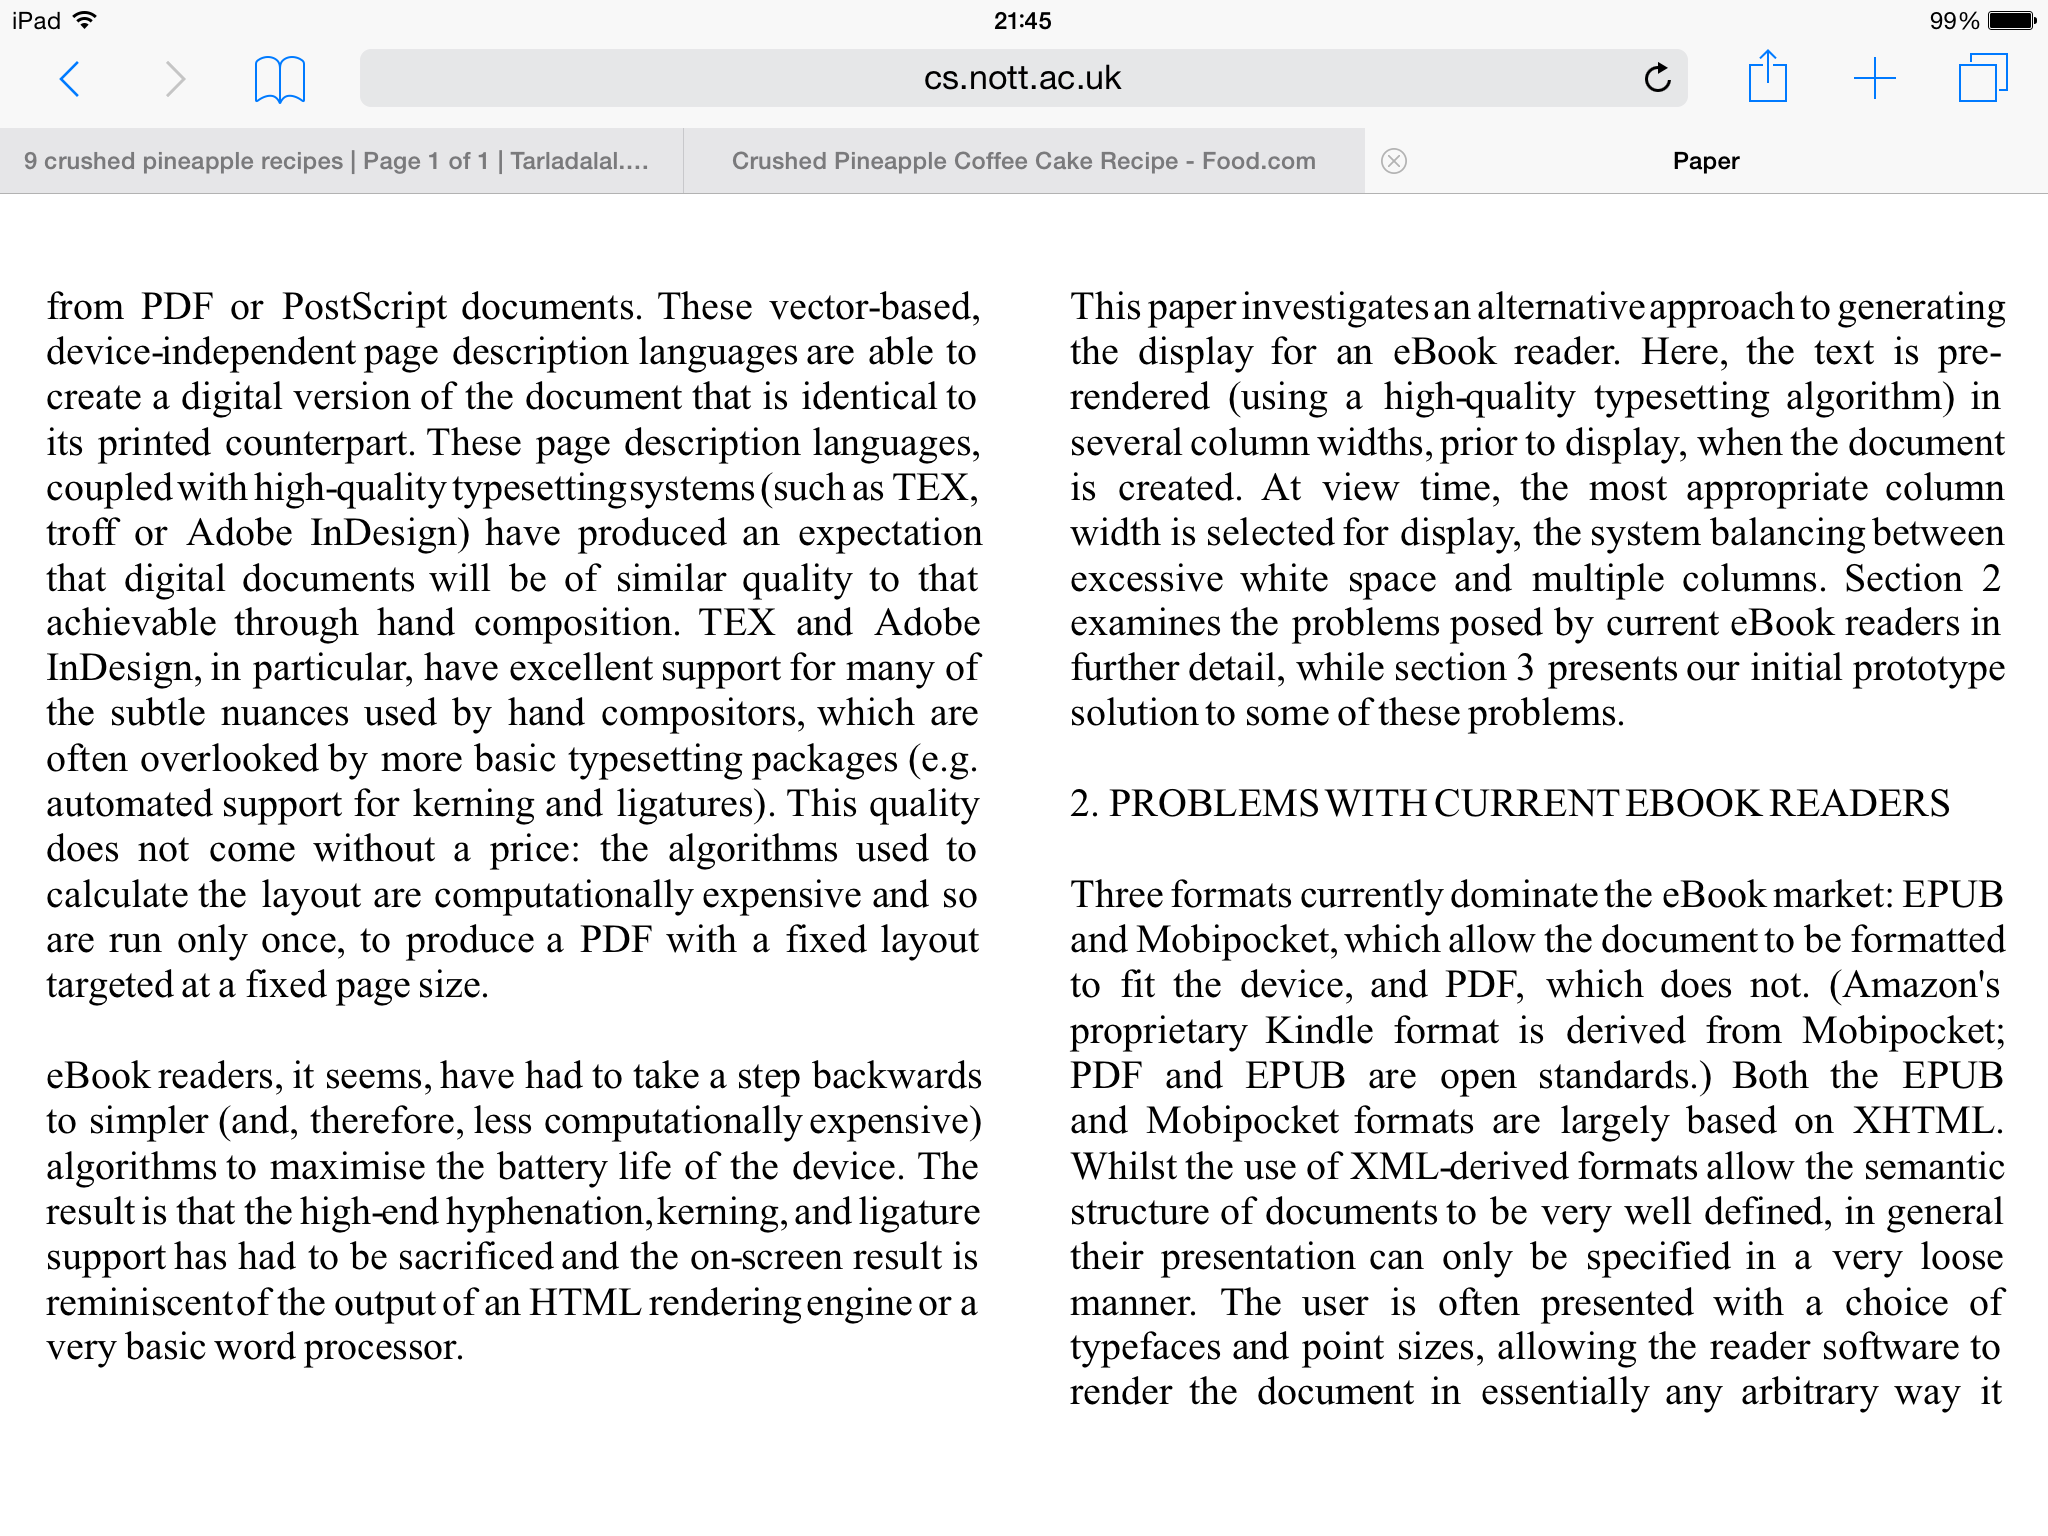
\includegraphics[width=\imgwid]{gfx/ipad-l3}}

\end{center}
\clearpage
\section{Other systems}
\label{app:layout-other}

\subsection{\LaTeX}

\cite{Pinkney2011} as rendered by \LaTeX. The layout is very similar to that produced by the malleable document system (see \ref{app:layout-ff}) though \LaTeX{} favours placing floats at the top of columns, rather than directly at their logical position.

\begin{center}
\setlength{\imgwid}{0.47\textwidth}
\fbox{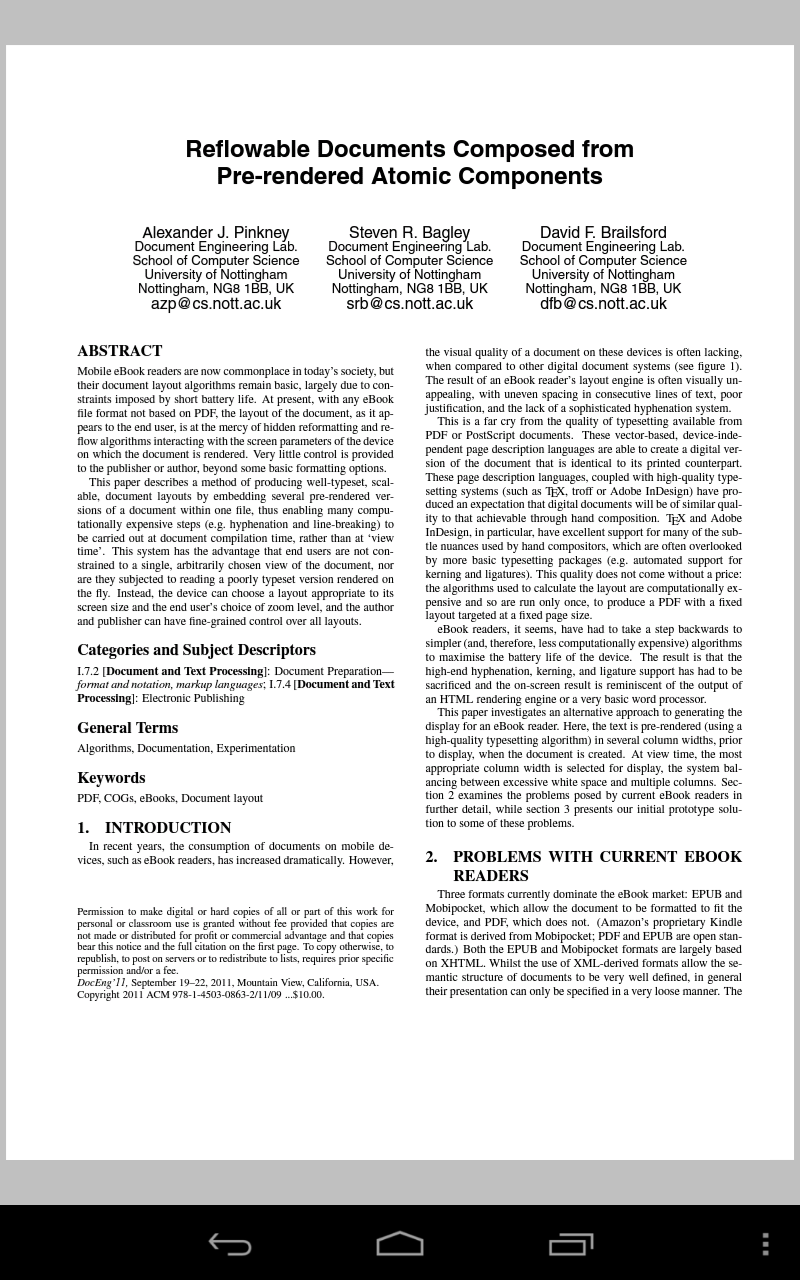
\includegraphics[trim=0.1in 2in 0.1in 1in, clip=true, width=\imgwid]{gfx/pbb11-1}}\hspace{0.01\textwidth}
\fbox{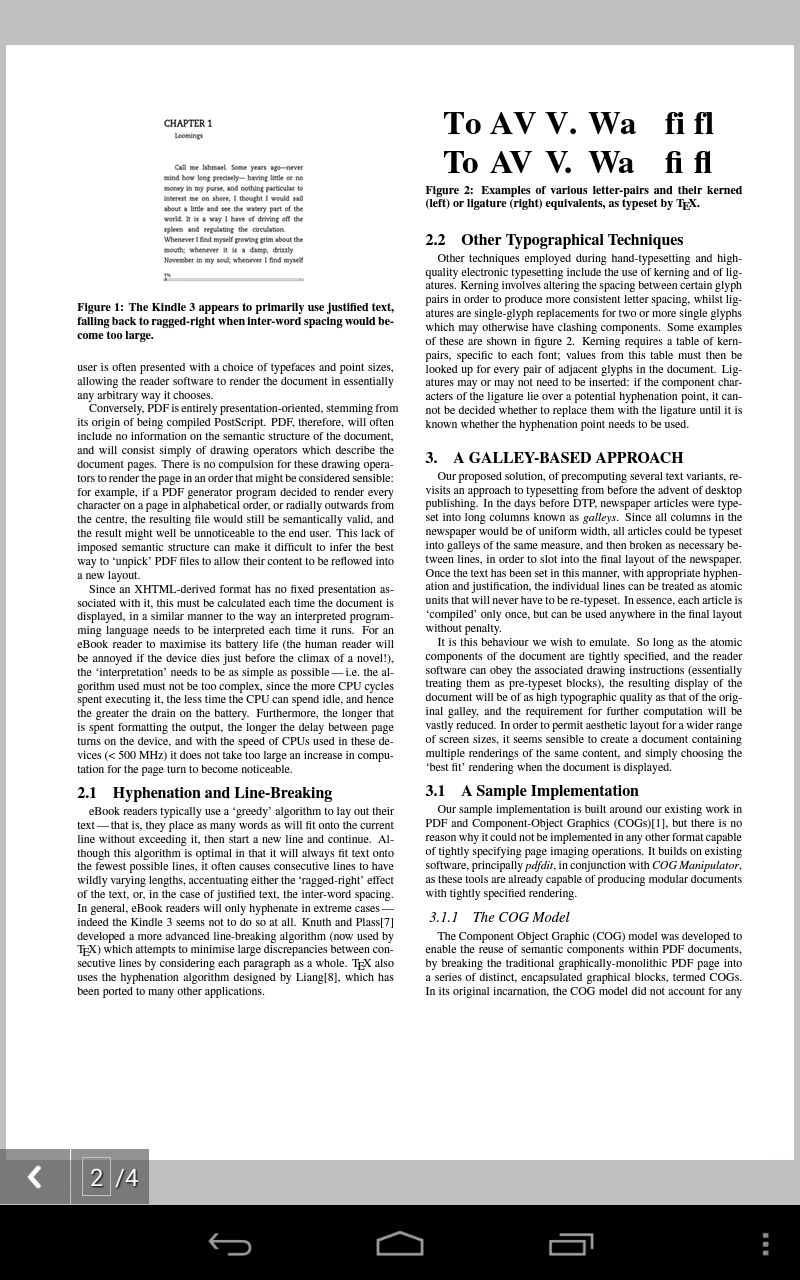
\includegraphics[trim=0.1in 2in 0.1in 1in, clip=true, width=\imgwid]{gfx/pbb11-2}}

\vspace{0.2in}
\fbox{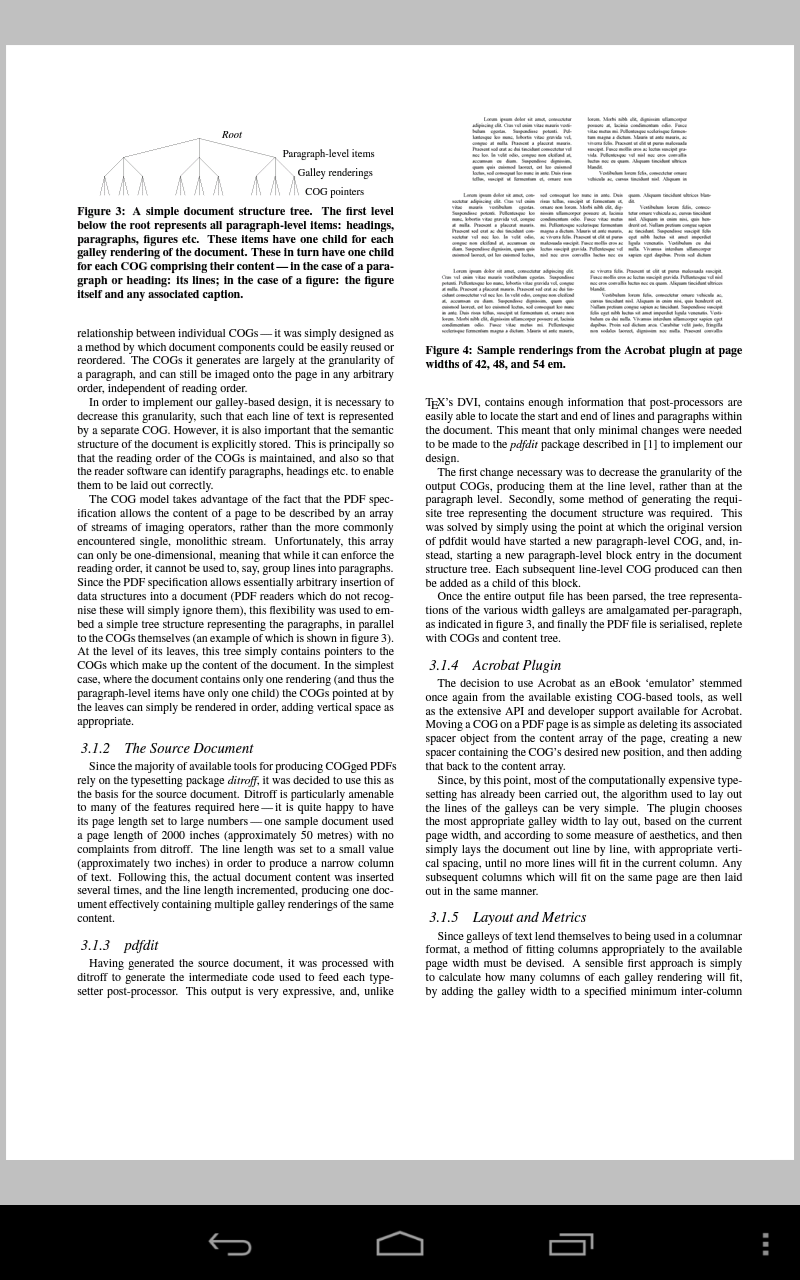
\includegraphics[trim=0.1in 2in 0.1in 1in, clip=true, width=\imgwid]{gfx/pbb11-3}}\hspace{0.01\textwidth}
\fbox{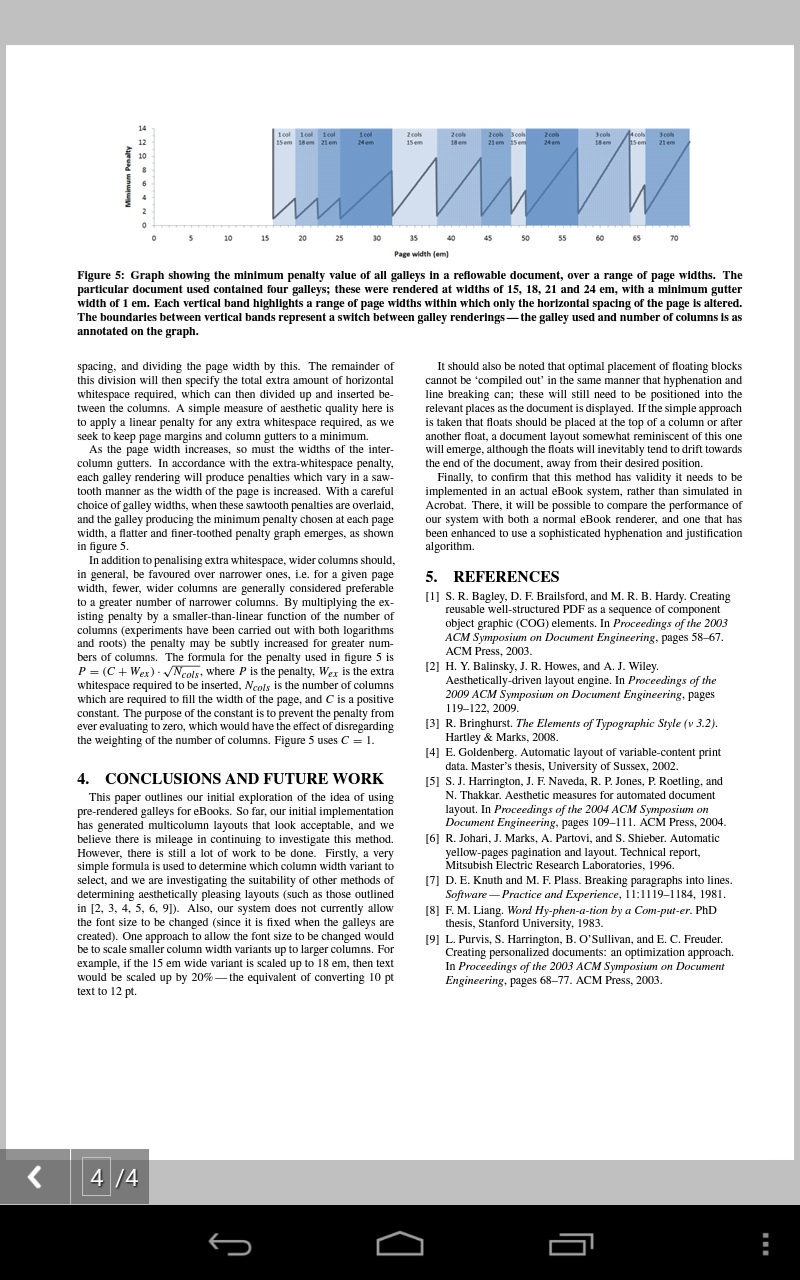
\includegraphics[trim=0.1in 2in 0.1in 1in, clip=true, width=\imgwid]{gfx/pbb11-4}}
\end{center}



\clearpage



\subsection{\textsc{html}}

\gls{html} version of \cite{Pinkney2011}, as rendered by Mozilla Firefox, scaled to fit multiple screen sizes. Though \gls{html} can stretch to any screen size, it tends to produce typographically inferior results, for example lines that are too long, or line breaking that results in extremely uneven spacing between adjacent lines.

\begin{center}
\setlength{\imgwid}{0.45\textwidth}
\fbox{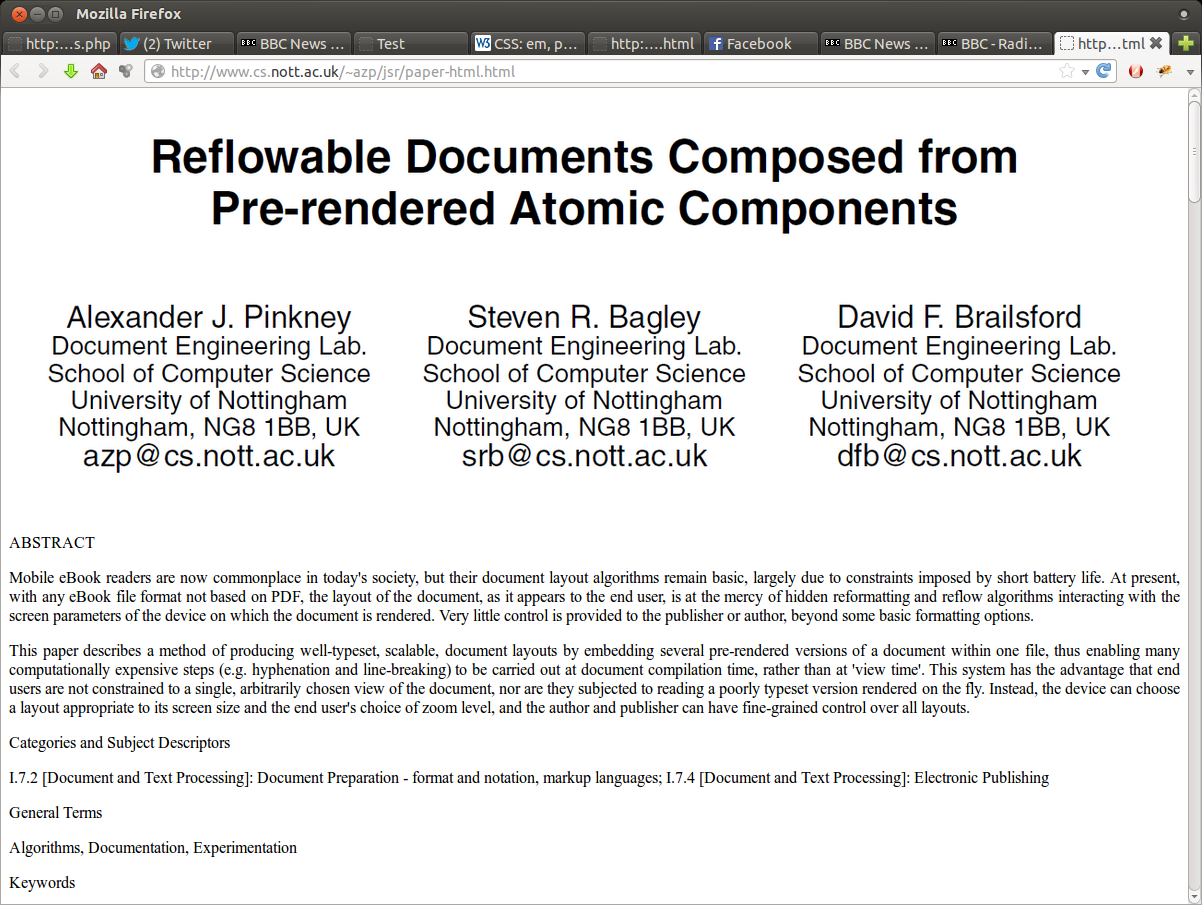
\includegraphics[trim=0in 0in 0in 1.2in, clip=true, width=\imgwid]{gfx/html1}}\hspace{0.01\textwidth}
\fbox{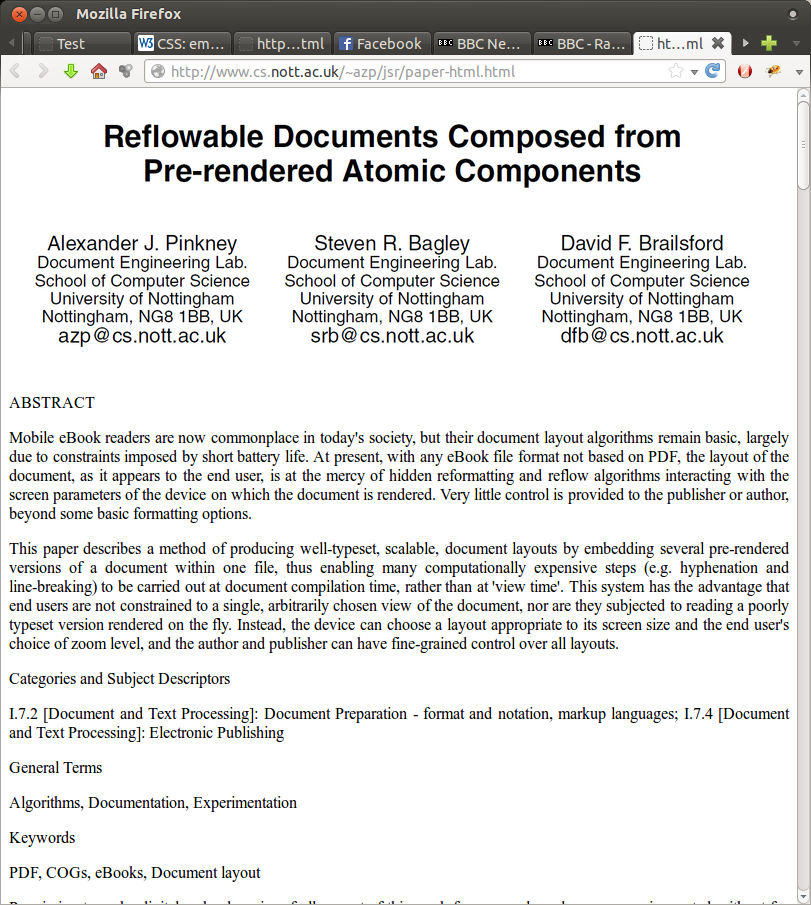
\includegraphics[trim=0in 0in 0in 1.2in, clip=true, width=\imgwid]{gfx/html2}}

\vspace{0.2in}
\fbox{\includegraphics[trim=0in 0in 0in 1.2in, clip=true, width=\imgwid]{gfx/html3}}\hspace{0.01\textwidth}
\fbox{\includegraphics[trim=0in 0in 0in 1.2in, clip=true, width=\imgwid]{gfx/html4}}
\end{center}


